\documentclass[compress]{beamer}
\usepackage{ifthen,verbatim}

\newcommand{\isnote}{}
\xdefinecolor{lightyellow}{rgb}{1.,1.,0.25}
\xdefinecolor{darkblue}{rgb}{0.1,0.1,0.7}

%% Uncomment this to get annotations
%% \def\notes{\addtocounter{page}{-1}
%%            \renewcommand{\isnote}{*}
%% 	   \beamertemplateshadingbackground{lightyellow}{white}
%%            \begin{frame}
%%            \frametitle{Notes for the previous page (page \insertpagenumber)}
%%            \itemize}
%% \def\endnotes{\enditemize
%% 	      \end{frame}
%%               \beamertemplateshadingbackground{white}{white}
%%               \renewcommand{\isnote}{}}

%% Uncomment this to not get annotations
\def\notes{\comment}
\def\endnotes{\endcomment}

\setbeamertemplate{navigation symbols}{}
\setbeamertemplate{headline}{\mbox{ } \hfill
\begin{minipage}{5.5 cm}
\vspace{-0.75 cm} \small
\end{minipage} \hfill
\begin{minipage}{4.5 cm}
\vspace{-0.75 cm} \small
\begin{flushright}
\ifthenelse{\equal{\insertpagenumber}{1}}{}{Jim Pivarski \hspace{0.2 cm} \insertpagenumber\isnote/\pageref{numpages}}
\end{flushright}
\end{minipage}\mbox{\hspace{0.2 cm}}\includegraphics[height=1 cm]{../cmslogo} \hspace{0.1 cm} \includegraphics[height=1 cm]{../tamulogo} \hspace{0.01 cm} \vspace{-1.05 cm}}

\begin{document}
\begin{frame}
\vfill
\begin{center}
\textcolor{darkblue}{\Large Confirmation of the Effect of RPC Hits \\ \vspace{0.2 cm} and Updated Alignment without RPC Bias}

\vfill
\begin{columns}
\column{0.3\linewidth}
\begin{center}
\large
\textcolor{darkblue}{\it Jim Pivarski}

Aysen Tatarinov

Vadim Khotilovich

Alexei Safonov
\end{center}
\end{columns}

\begin{columns}
\column{0.3\linewidth}
\begin{center}
\scriptsize
{\it Texas A\&M University}
\end{center}
\end{columns}

\vfill
28 May, 2010

\end{center}
\end{frame}

%% \begin{notes}
%% \item This is the annotated version of my talk.
%% \item If you want the version that I am presenting, download the one
%% labeled ``slides'' on Indico (or just ignore these yellow pages).
%% \item The annotated version is provided for extra detail and a written
%% record of comments that I intend to make orally.
%% \item Yellow notes refer to the content on the {\it previous} page.
%% \item All other slides are identical for the two versions.
%% \end{notes}

\small

% Muon TDR Figure 5.1.1a: locations of RPC chambers

\begin{frame}
\frametitle{First\ldots}

\begin{center}
\textcolor{darkblue}{\Huge Thank you, Pablo!}

\vfill
\Large The inclusion of RPC hits in the track refits was the cause of most muon alignment mysteries
\end{center}

%% \begin{itemize}\setlength{\itemsep}{0.75 cm}
%% \item 
%% \end{itemize}
%% \hspace{-0.83 cm} \textcolor{darkblue}{\Large Outline2}
\end{frame}

\begin{frame}
\frametitle{Pablo's Grand Unified Theory}
\framesubtitle{of Muon Track Residuals Mysteries}
Yesterday morning, none of the following were understood; \\ now they all are

\begin{itemize}\setlength{\itemsep}{0.2 cm}
\item Sawtooth effect: why are there discontinuities at DT borders?

\textcolor{darkblue}{\it Because RPC borders are at the same place as DT borders}

\item Why does it depend on momentum, like an input-track bias?

\textcolor{darkblue}{\it Because the input tracks are biased--- by the RPCs, not tracker}

\item Why do we see it most strongly in ME1/2 with collisions muons?

\textcolor{darkblue}{\it Because that's where the RPCs are in the endcap}

\item Why does tracker weak-mode effect have a characteristic scale of
  100~GeV/$c$, even with a scale-invariant tracker weak mode?

\textcolor{darkblue}{\it Because the distance of the RPCs to the beamline, their
  resolution, and the CMS magnetic field set a characteristic scale of
  about 100~GeV/$c$, not the tracker weak mode}

\end{itemize}
\end{frame}

\begin{frame}
\frametitle{How did this happen?}
\begin{description}\setlength{\itemsep}{0.3 cm}
\item[Feb 2007:] Discovered that RPC hits were biasing the track refits

\item[Aug 2007:] ``RefitRPCHits'' switch integrated into CMSSW; track
  refits are unbiased by RPC hits when set to ``False''

\item[$\begin{array}{c} \mbox{sometime} \\ \mbox{thereafter:} \end{array}$] Made the following mistake in Python configuration file:

TrackRefitter.RefitRPCHits = False

\hfill \textcolor{red}{\it \# CMSSW doesn't complain; uses default (True)}

\vspace{0.25 cm}
instead of

\vspace{0.25 cm}
\textcolor{gray}{TrackRefitter}.TrackTransformer.\textcolor{gray}{RefitRPCHits = False}

\hfill \textcolor{red}{\it \# what we want}
\end{description}

\textcolor{darkblue}{RPC hits were being included in track refits because of a typo}
\end{frame}

\begin{frame}
\frametitle{Conclusions}
\framesubtitle{(will be repeated at the end of this talk)}
\begin{itemize}
\item Confirmation: sawtooth and dependence on $q/p_T$ disappear when tracks unbiased by RPC hits
\begin{itemize}
\item $p_T > 100$~GeV/$c$ cut limits effect on alignment results
\end{itemize}

\item We do not see large $\vec{B}$ field bias: less than 1\% before station~1

\item Modified interpretation of tracker weak modes
\begin{itemize}
\item no more ``high-momentum vs.\ low-momentum'' discrepancy
\item muon residuals cannot probe tracker weak modes
\item cosmic endpoint constraint on tracker weak modes $\Rightarrow$
  $\sim$0.25~mm bias in chamber $x$ positions
\end{itemize}

\item New 2010 muon alignment without RPC bias
\begin{itemize}
\item RPC bias effectively a 0.3~mrad rotation and 1.5~mm chamber position error
\item unrelated to ``twist'' with respect to hardware geometry
\end{itemize}

\item We no longer need the $p_T > 100$~GeV/$c$ cut, which will make alignments with collisions possible
\begin{itemize}
\item resolution vs.\ integrated luminosity estimates must be revised
\end{itemize}
\end{itemize}
\end{frame}

\begin{frame}
\frametitle{Sawtooth (confirmation)}
\framesubtitle{``high-$p_T$'' means $p_T > 100$~GeV/$c$, ``low-$p_T$'' means $20 < p_T < 100$~GeV/$c$}

\only<3-4>{RPC hits shouldn't affect local $y$ or $dy/dz$ residuals}

\begin{columns}
\column{0.5\linewidth}
\begin{center}
track refits biased by RPC hits
\end{center}
\only<1>{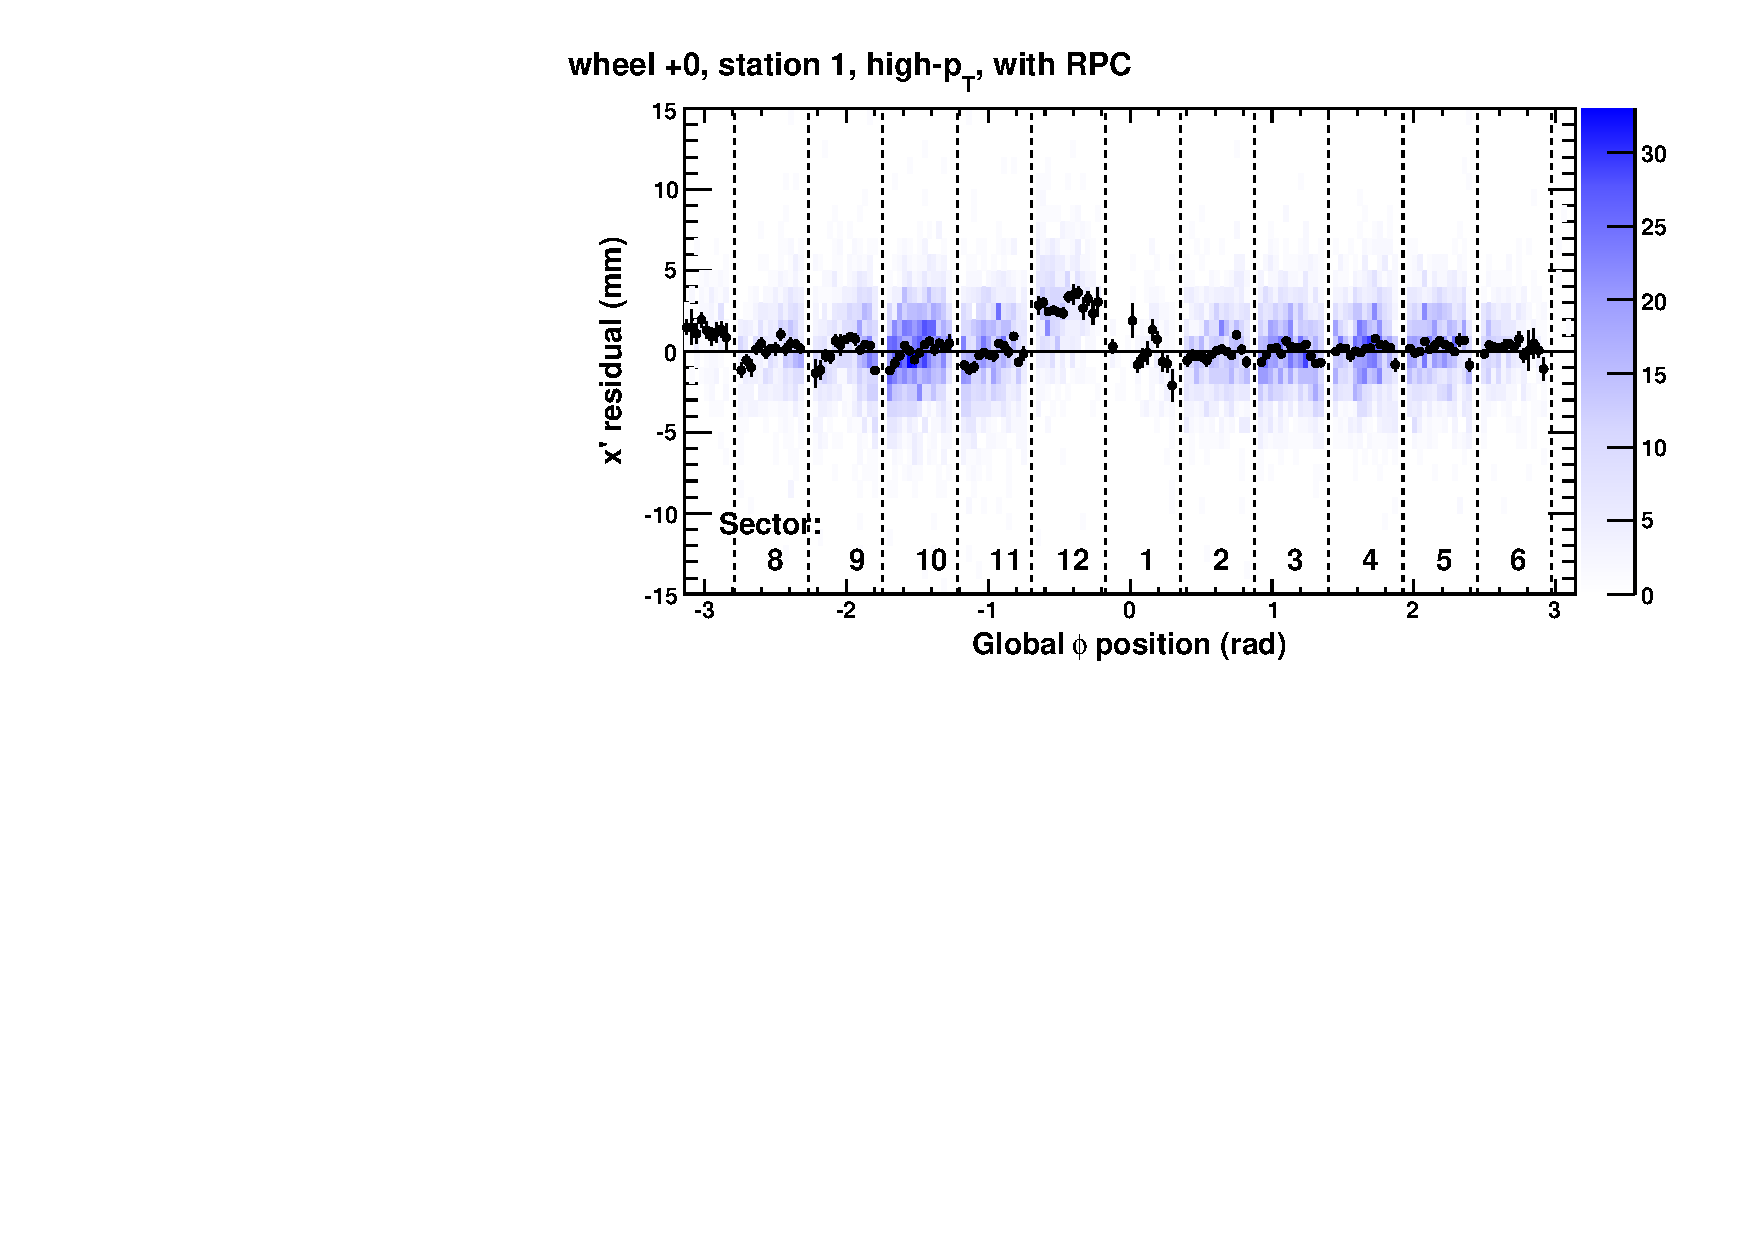
\includegraphics[width=\linewidth]{sawtoothexample_x_high_withrpc.pdf}}

\only<1>{\fbox{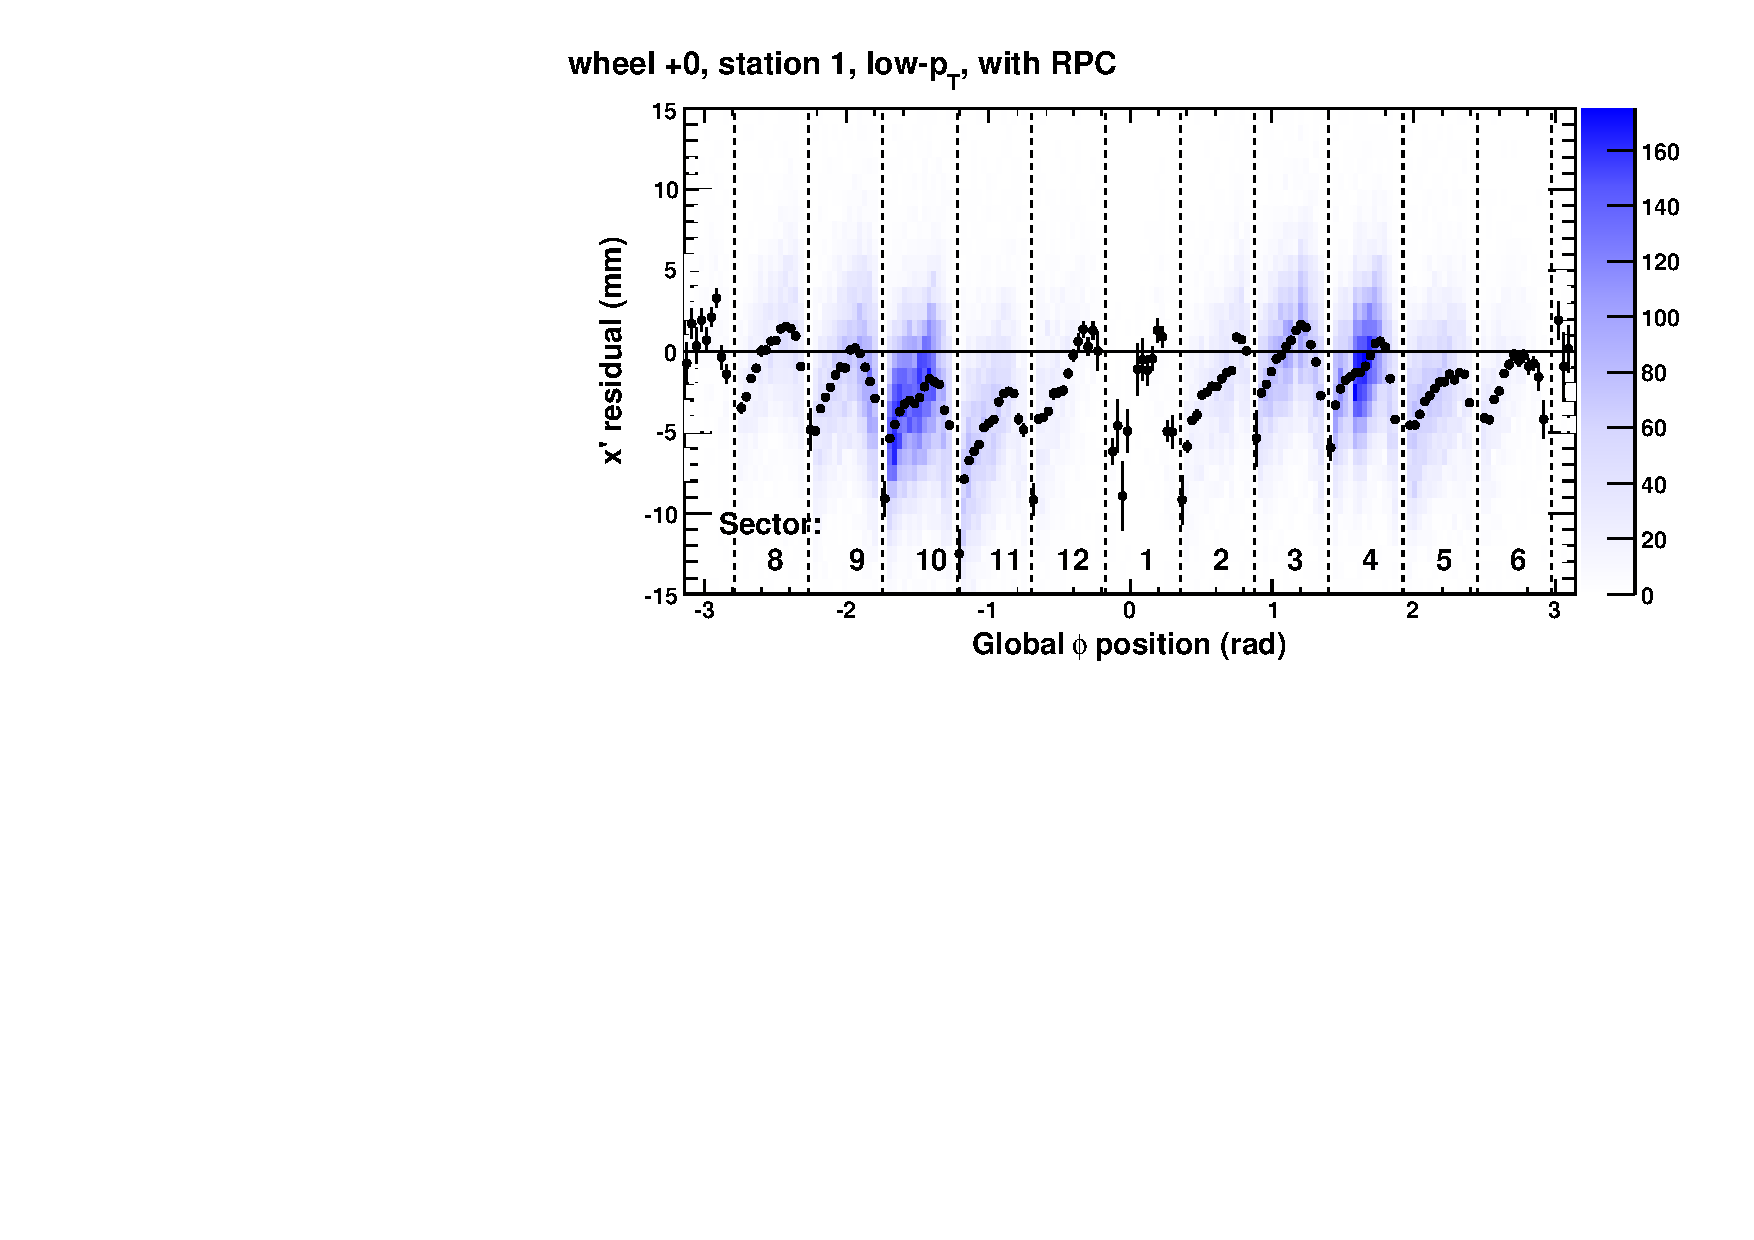
\includegraphics[width=\linewidth]{sawtoothexample_x_low_withrpc.pdf}}}

\only<2>{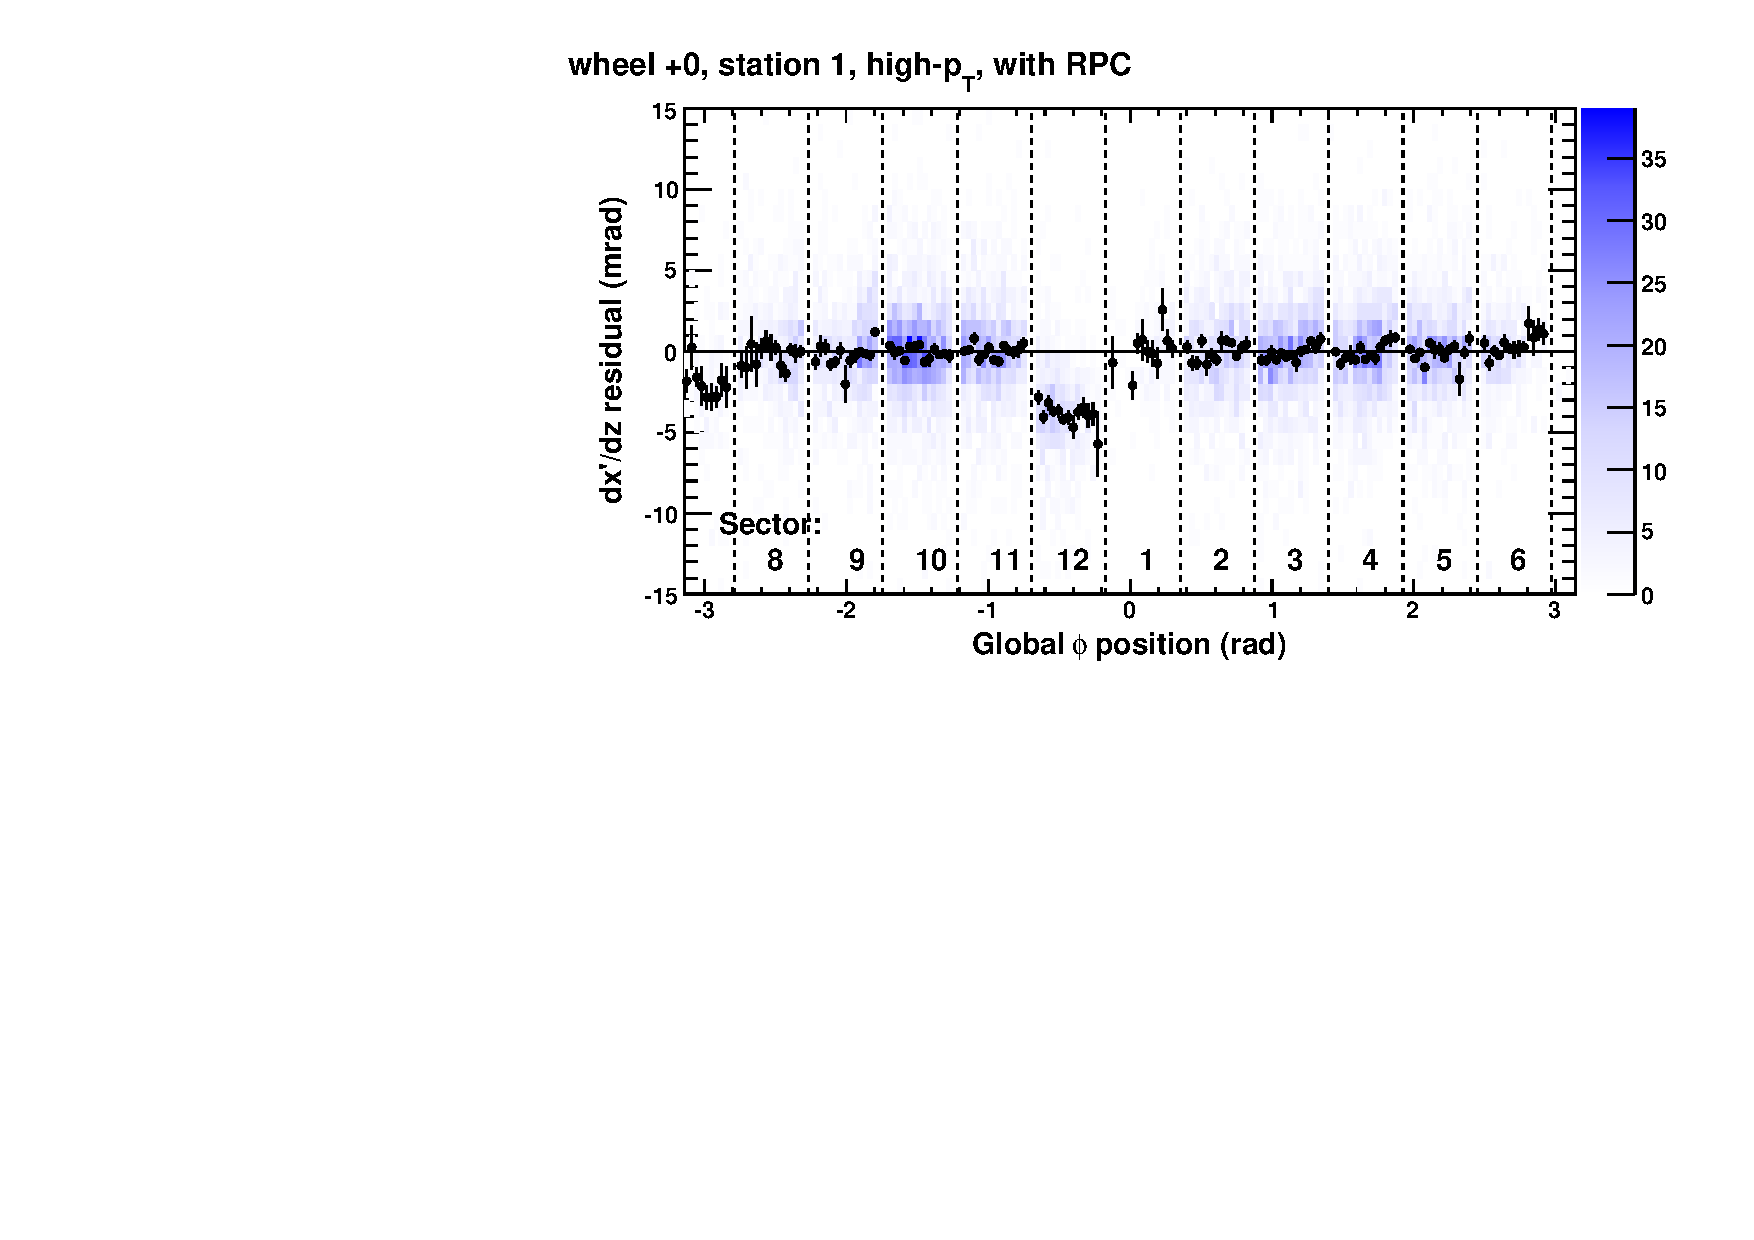
\includegraphics[width=\linewidth]{sawtoothexample_dxdz_high_withrpc.pdf}}

\only<2>{\fbox{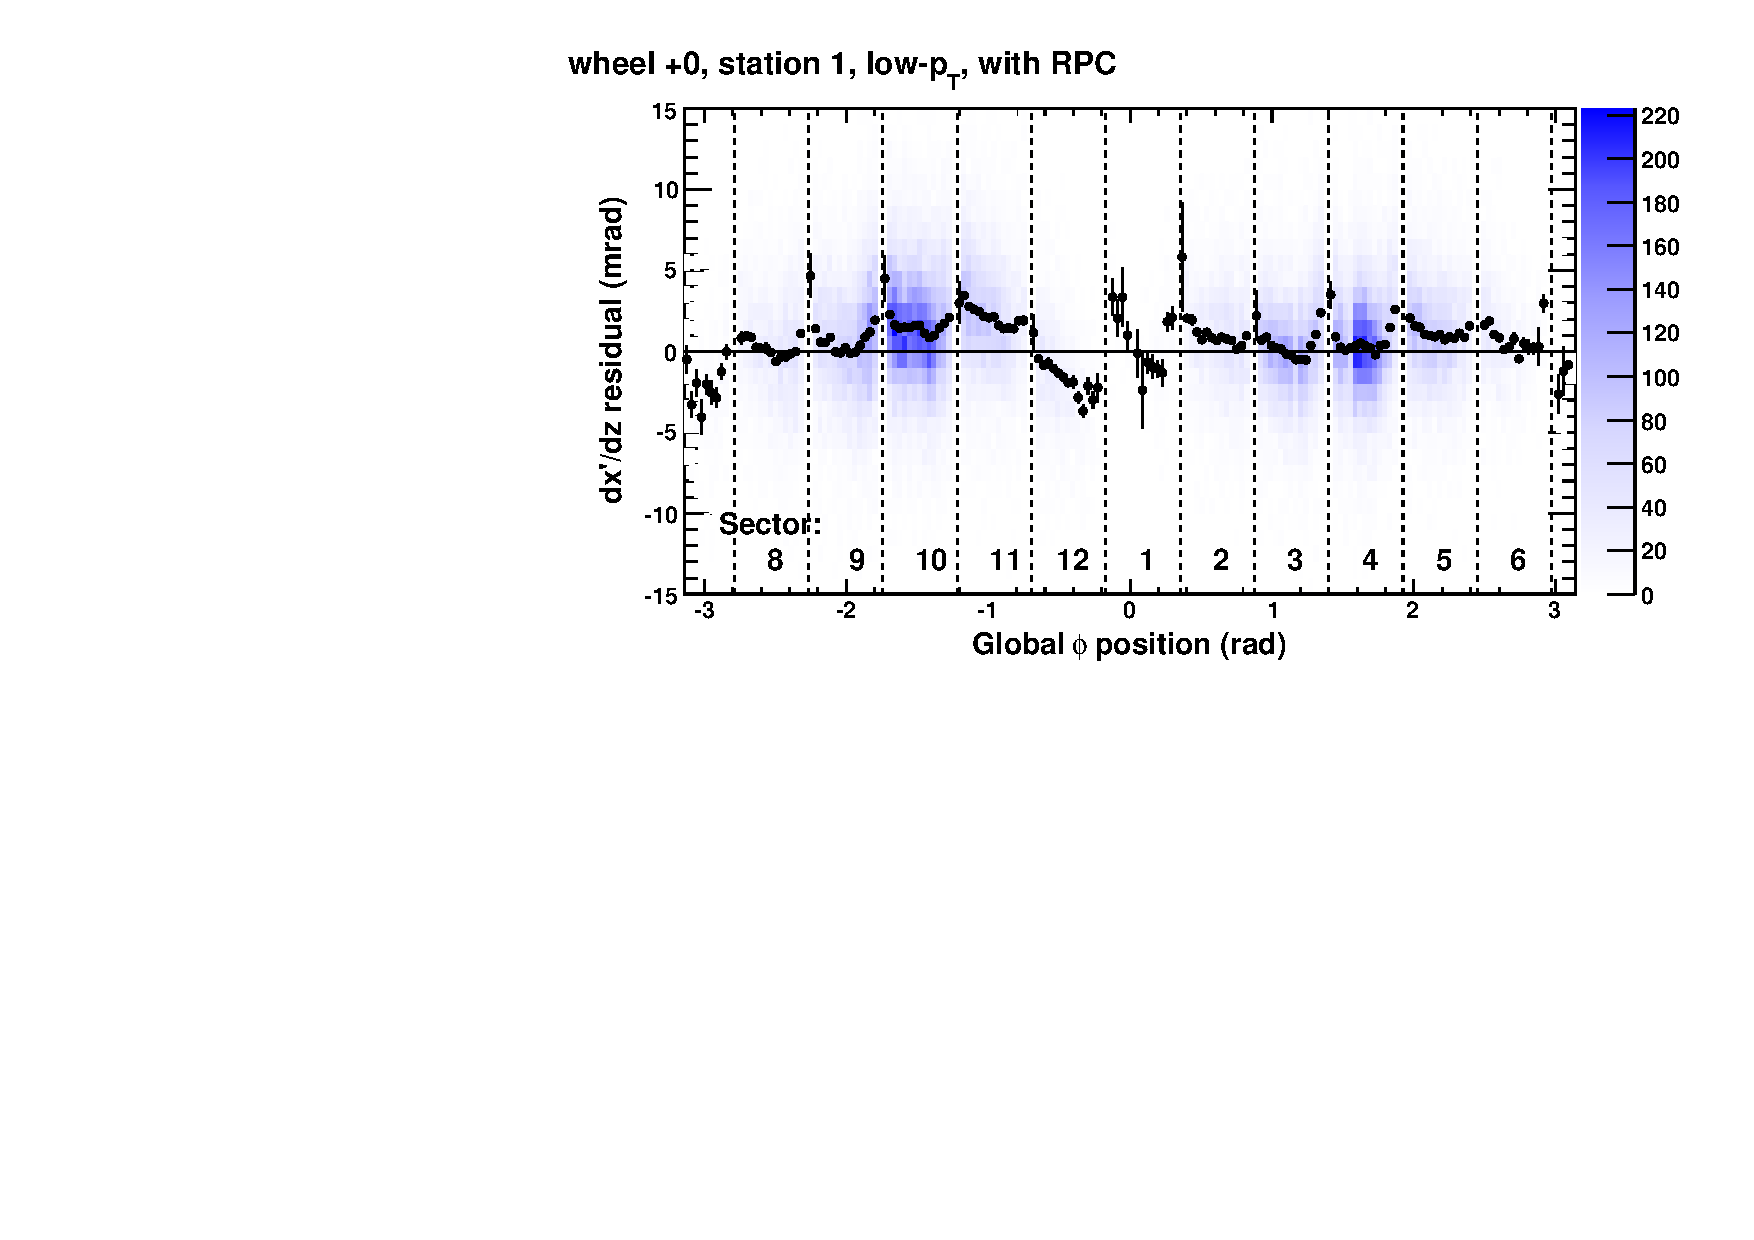
\includegraphics[width=\linewidth]{sawtoothexample_dxdz_low_withrpc.pdf}}}

\only<3>{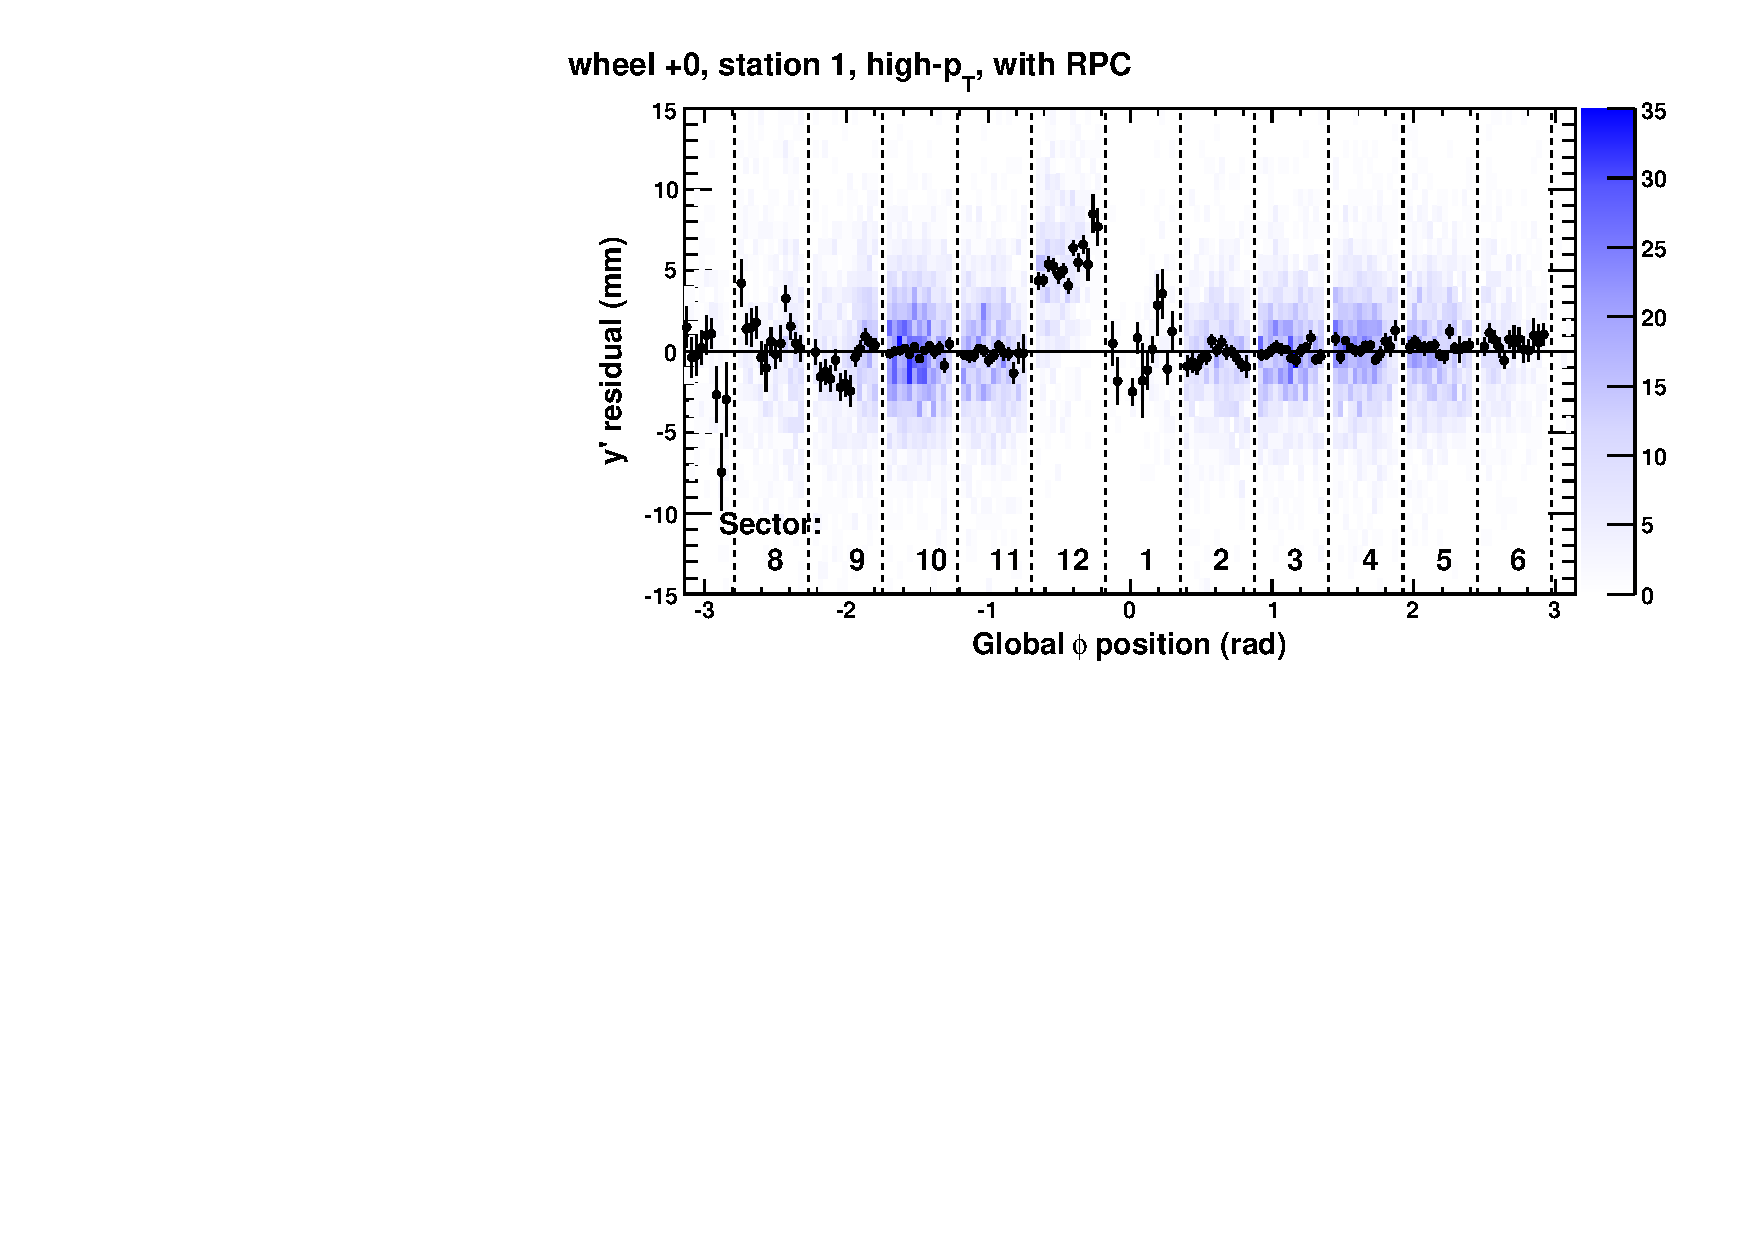
\includegraphics[width=\linewidth]{sawtoothexample_y_high_withrpc.pdf}}

\only<3>{\fbox{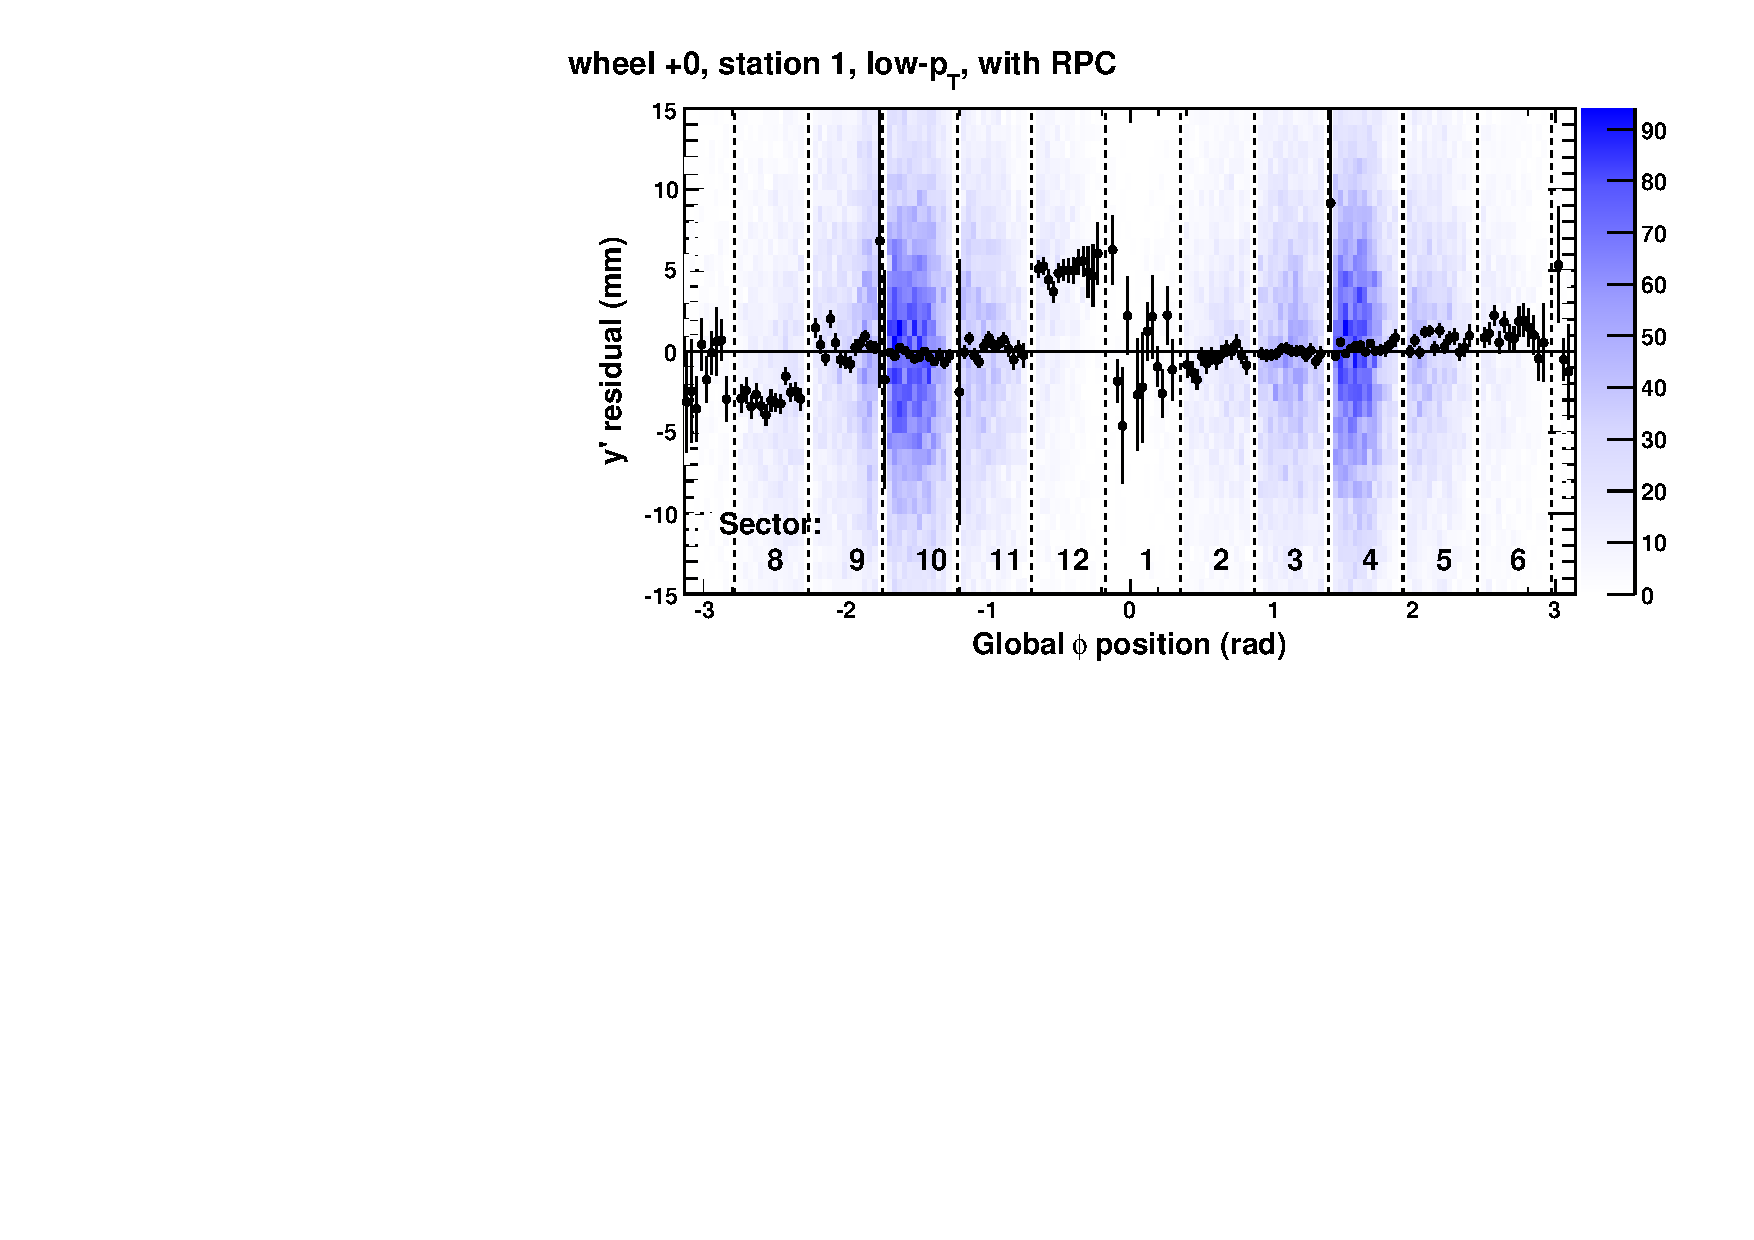
\includegraphics[width=\linewidth]{sawtoothexample_y_low_withrpc.pdf}}}

\only<4>{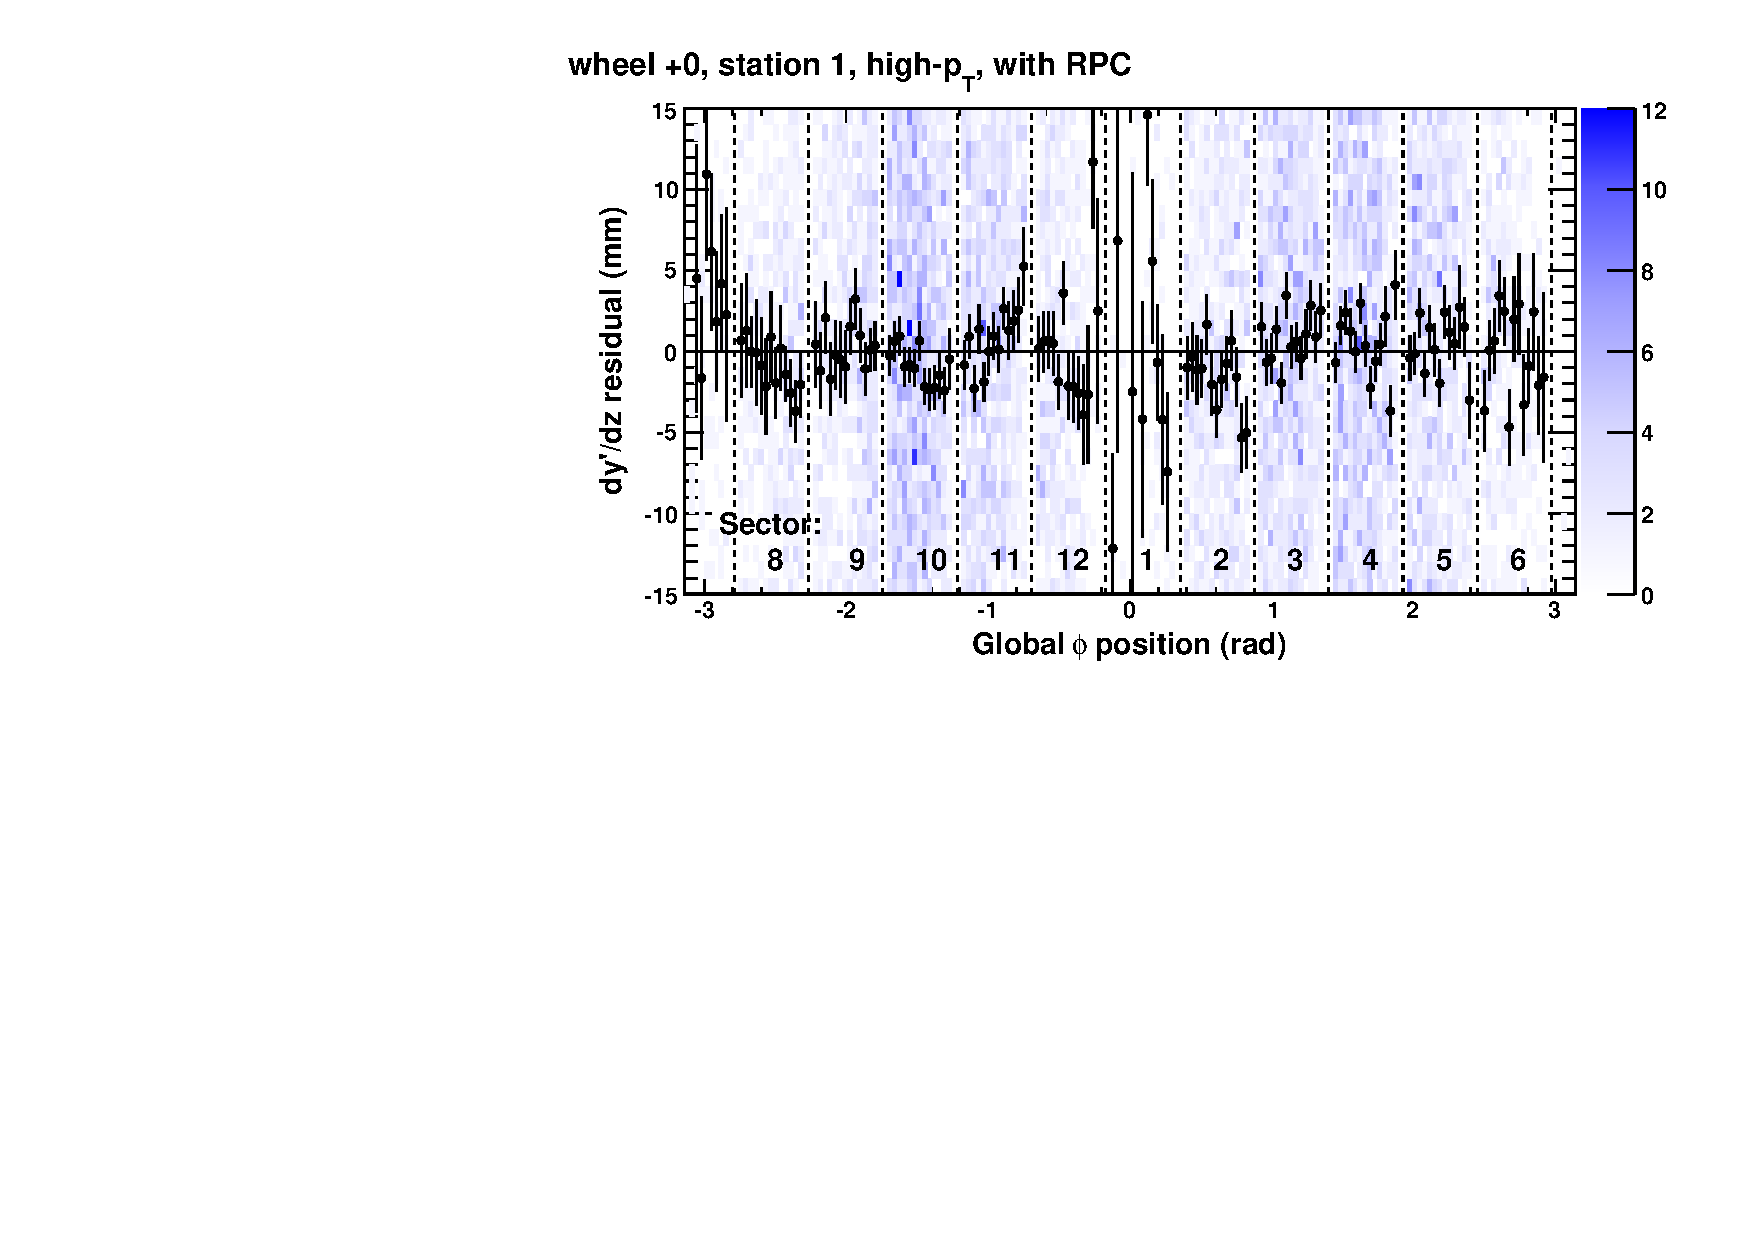
\includegraphics[width=\linewidth]{sawtoothexample_dydz_high_withrpc.pdf}}

\only<4>{\fbox{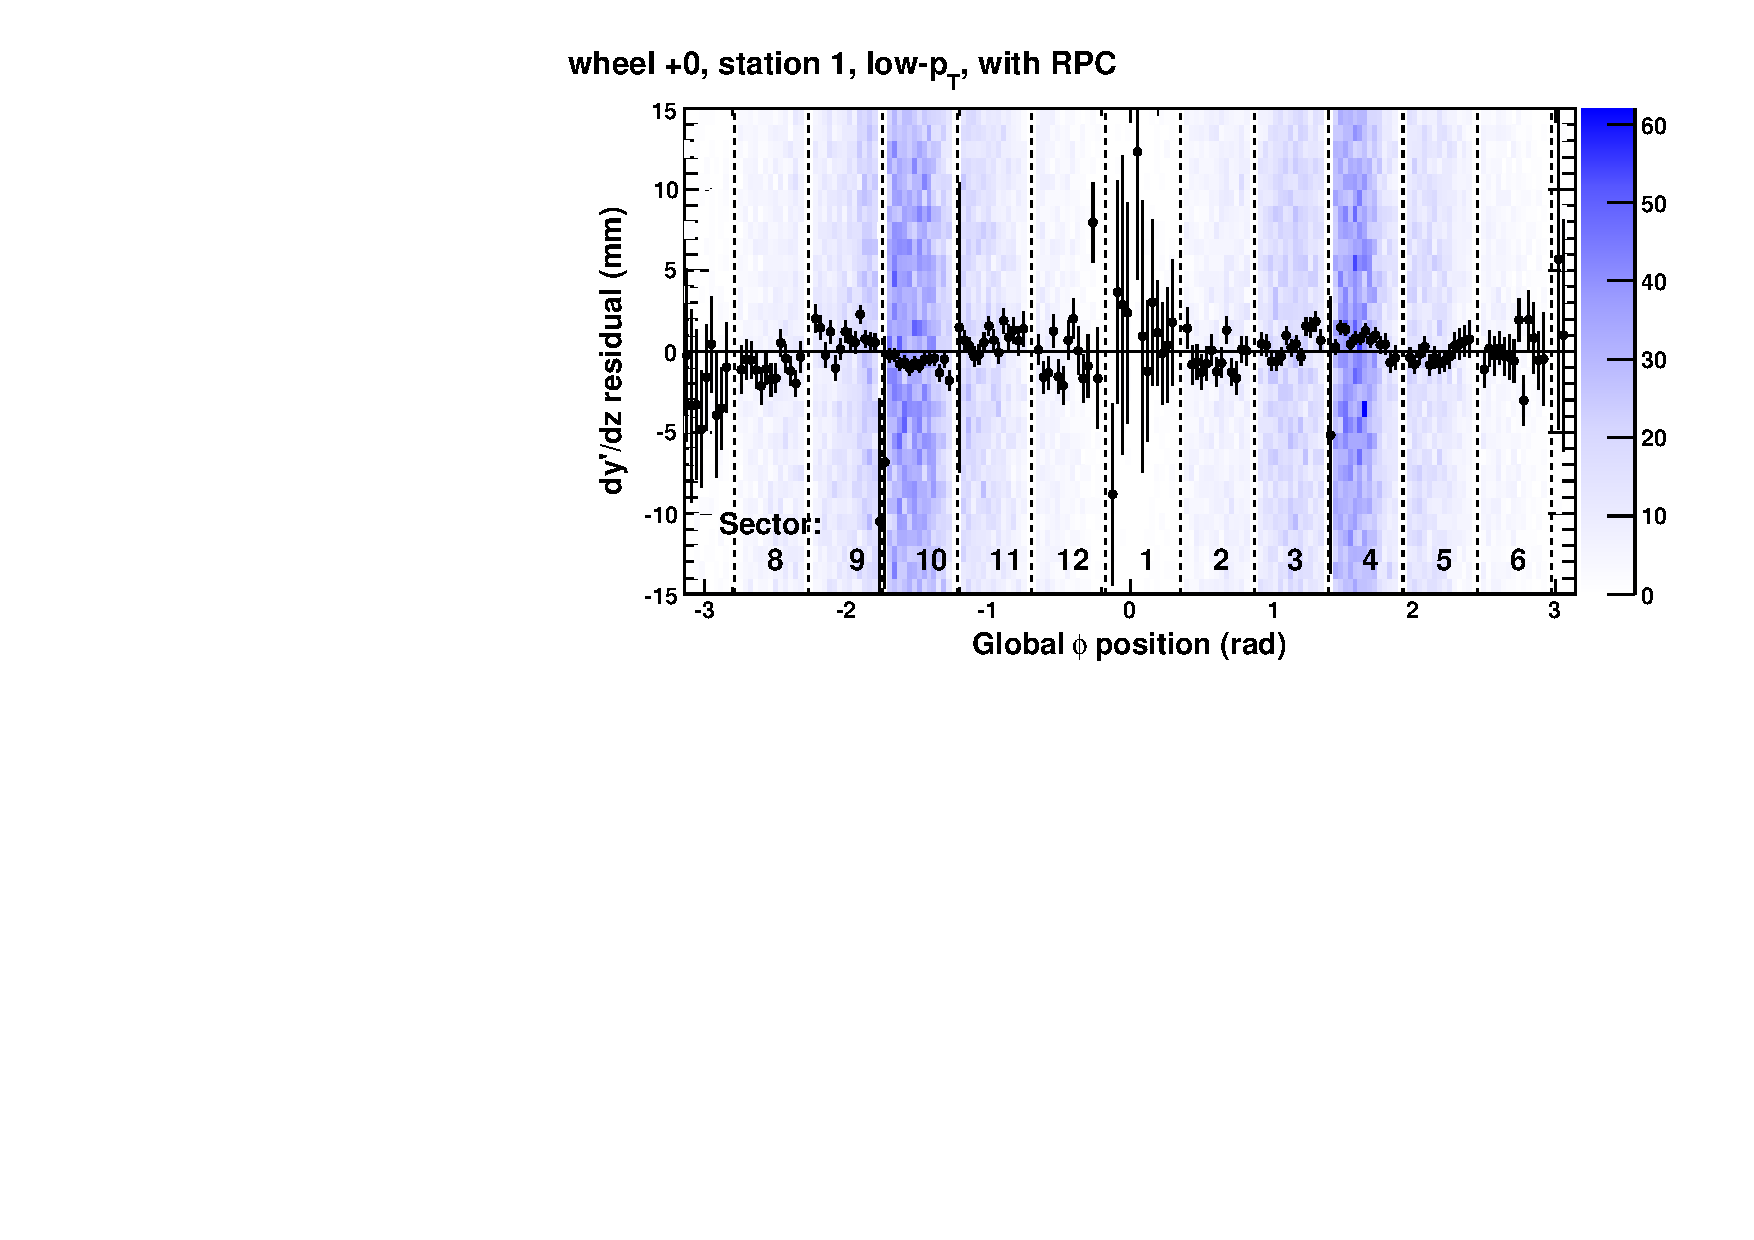
\includegraphics[width=\linewidth]{sawtoothexample_dydz_low_withrpc.pdf}}}

\column{0.5\linewidth}
\begin{center}
unbiased track refits
\end{center}
\only<1>{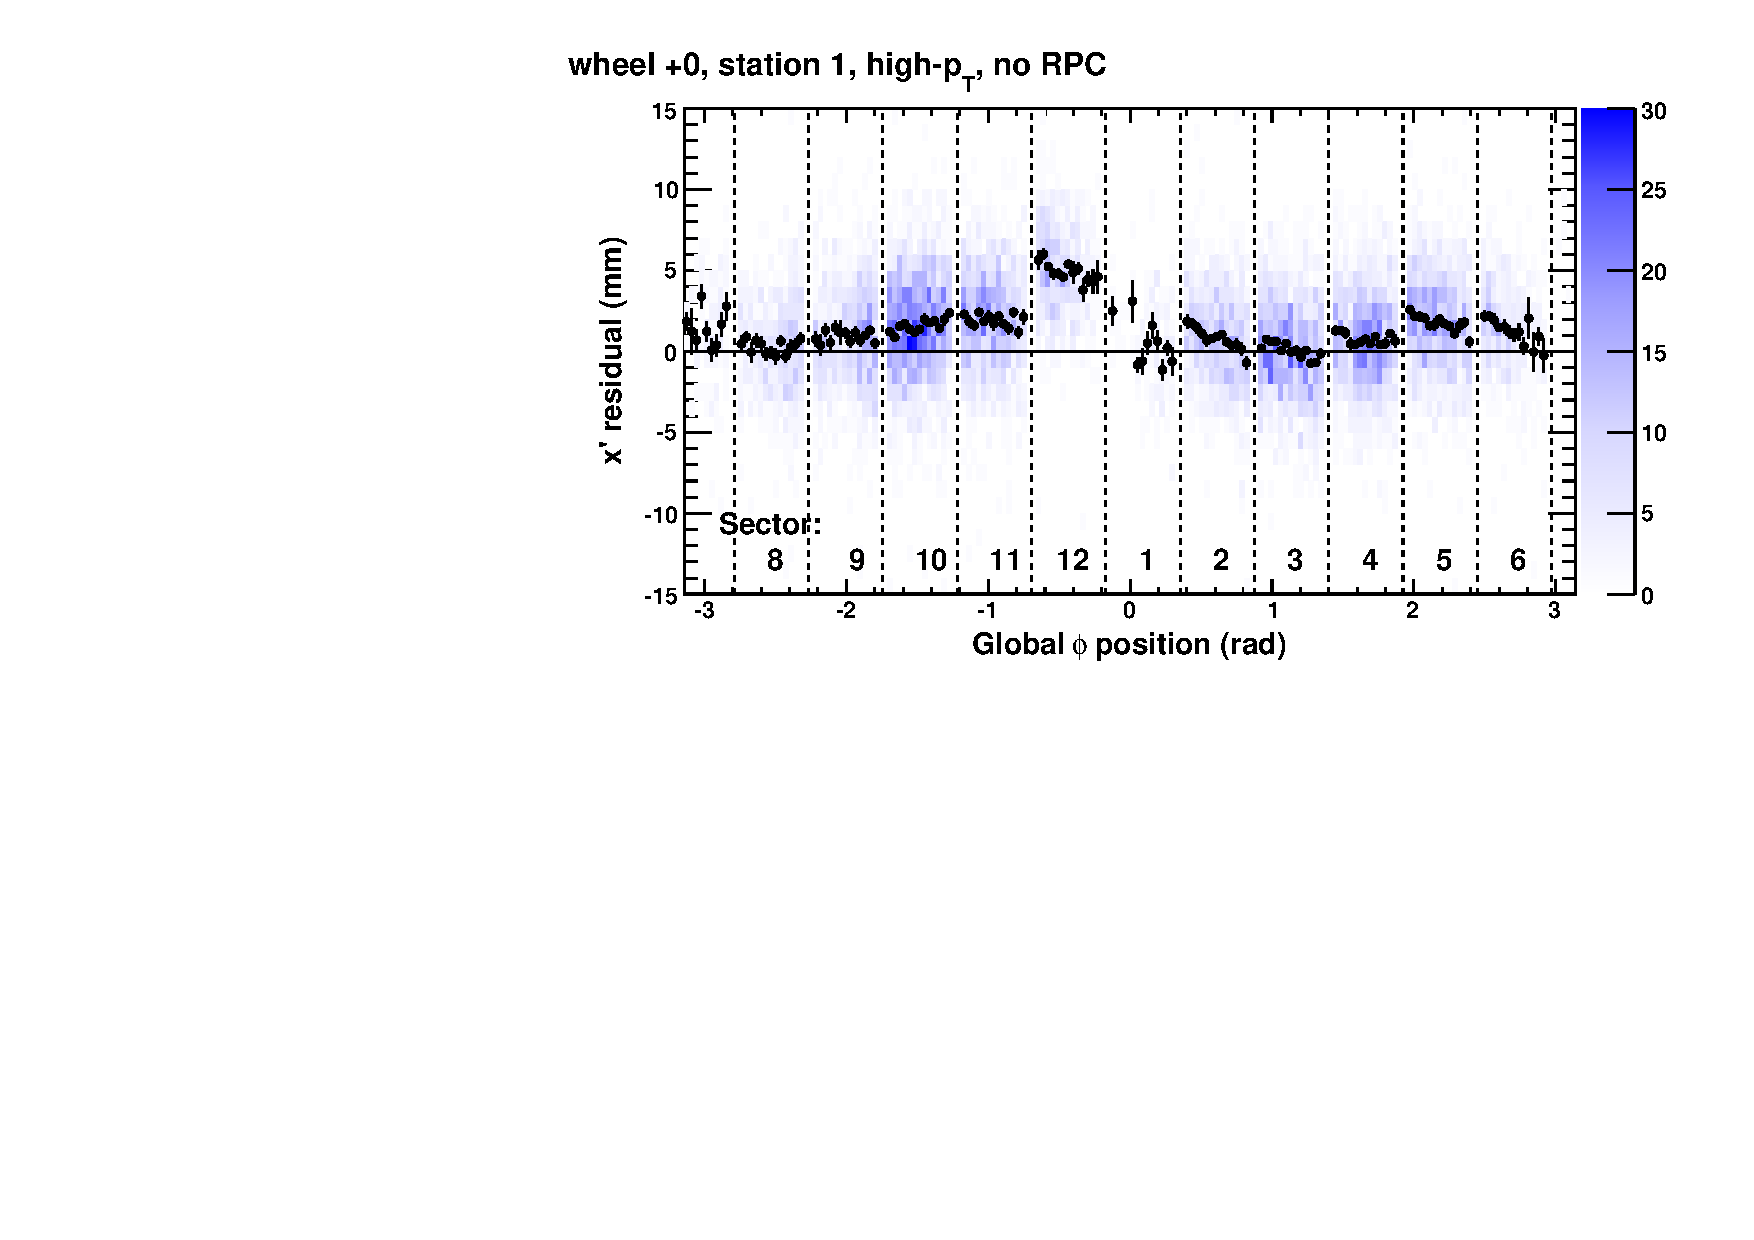
\includegraphics[width=\linewidth]{sawtoothexample_x_high_norpc.pdf}}

\only<1>{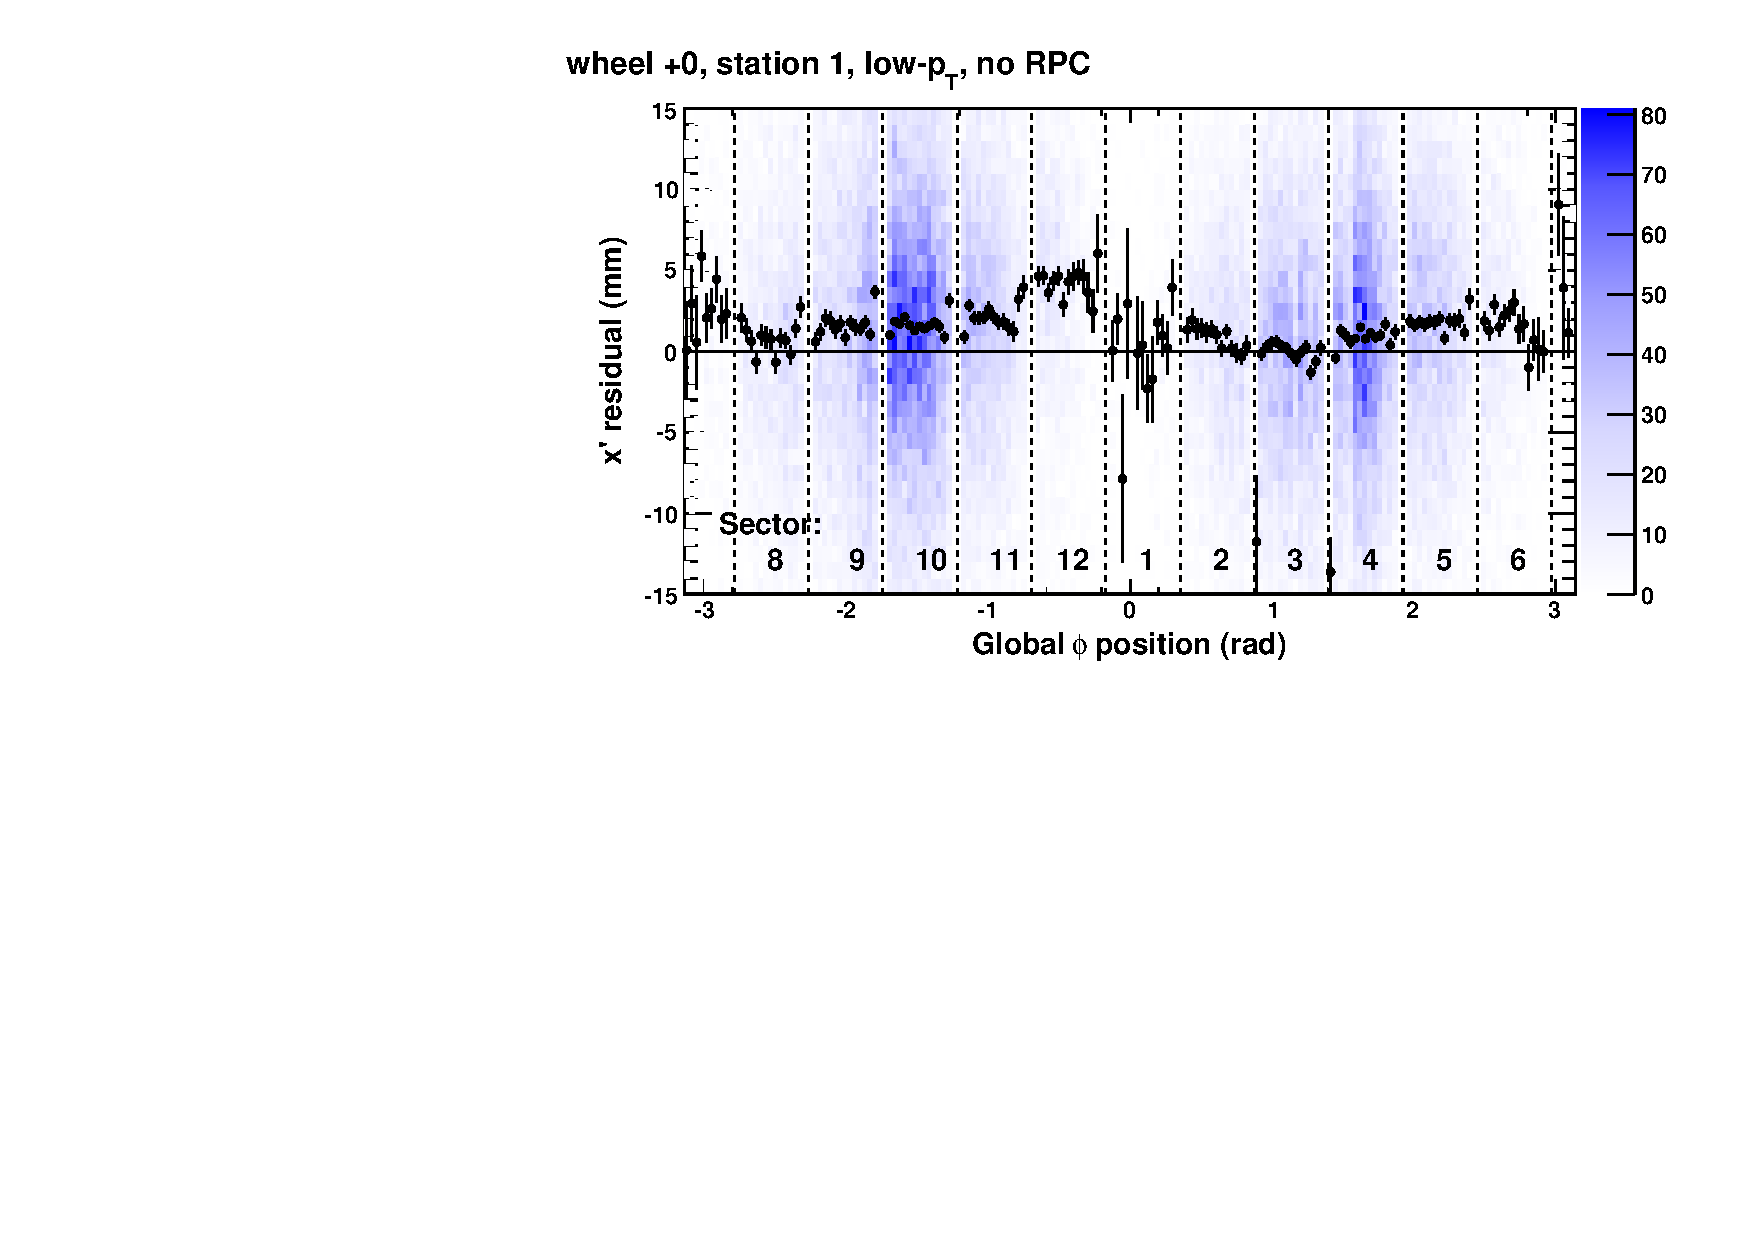
\includegraphics[width=\linewidth]{sawtoothexample_x_low_norpc.pdf}}

\only<2>{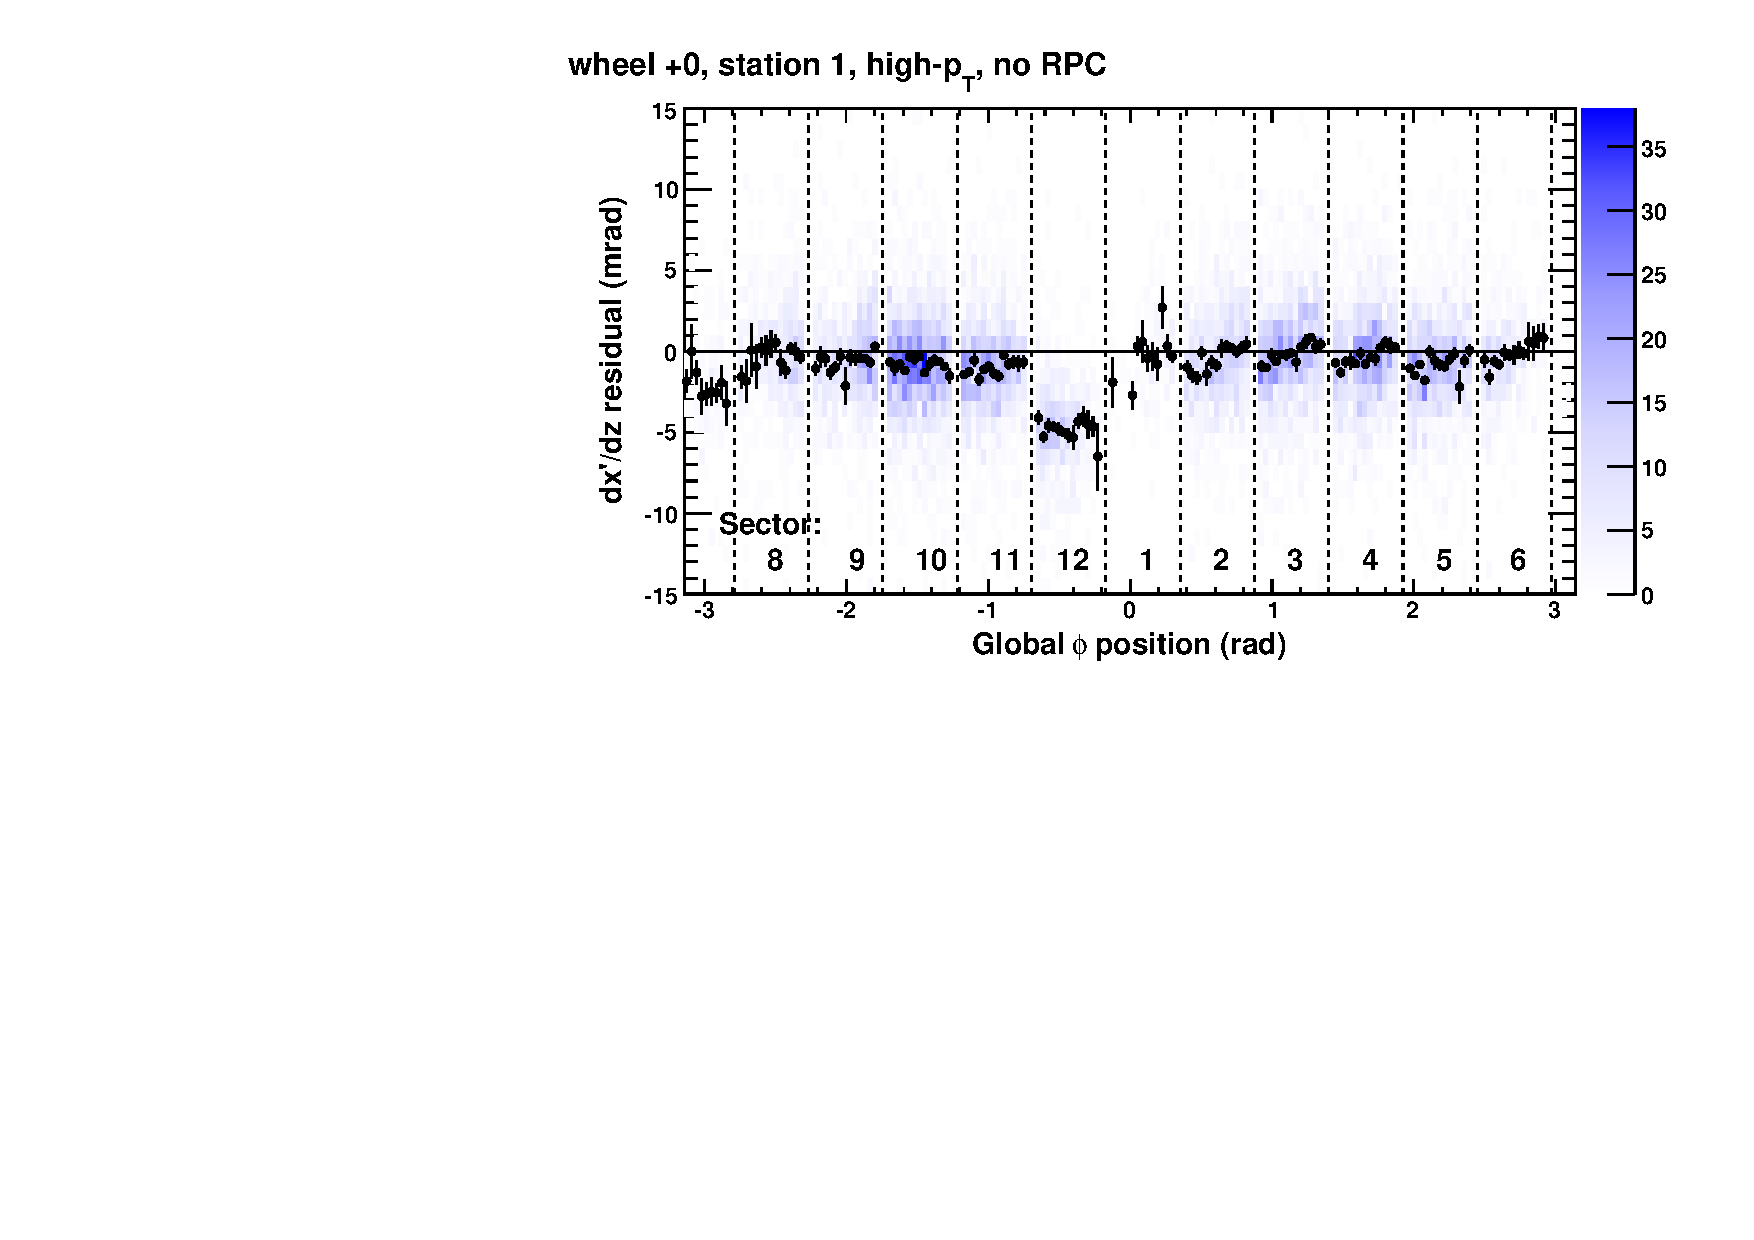
\includegraphics[width=\linewidth]{sawtoothexample_dxdz_high_norpc.pdf}}

\only<2>{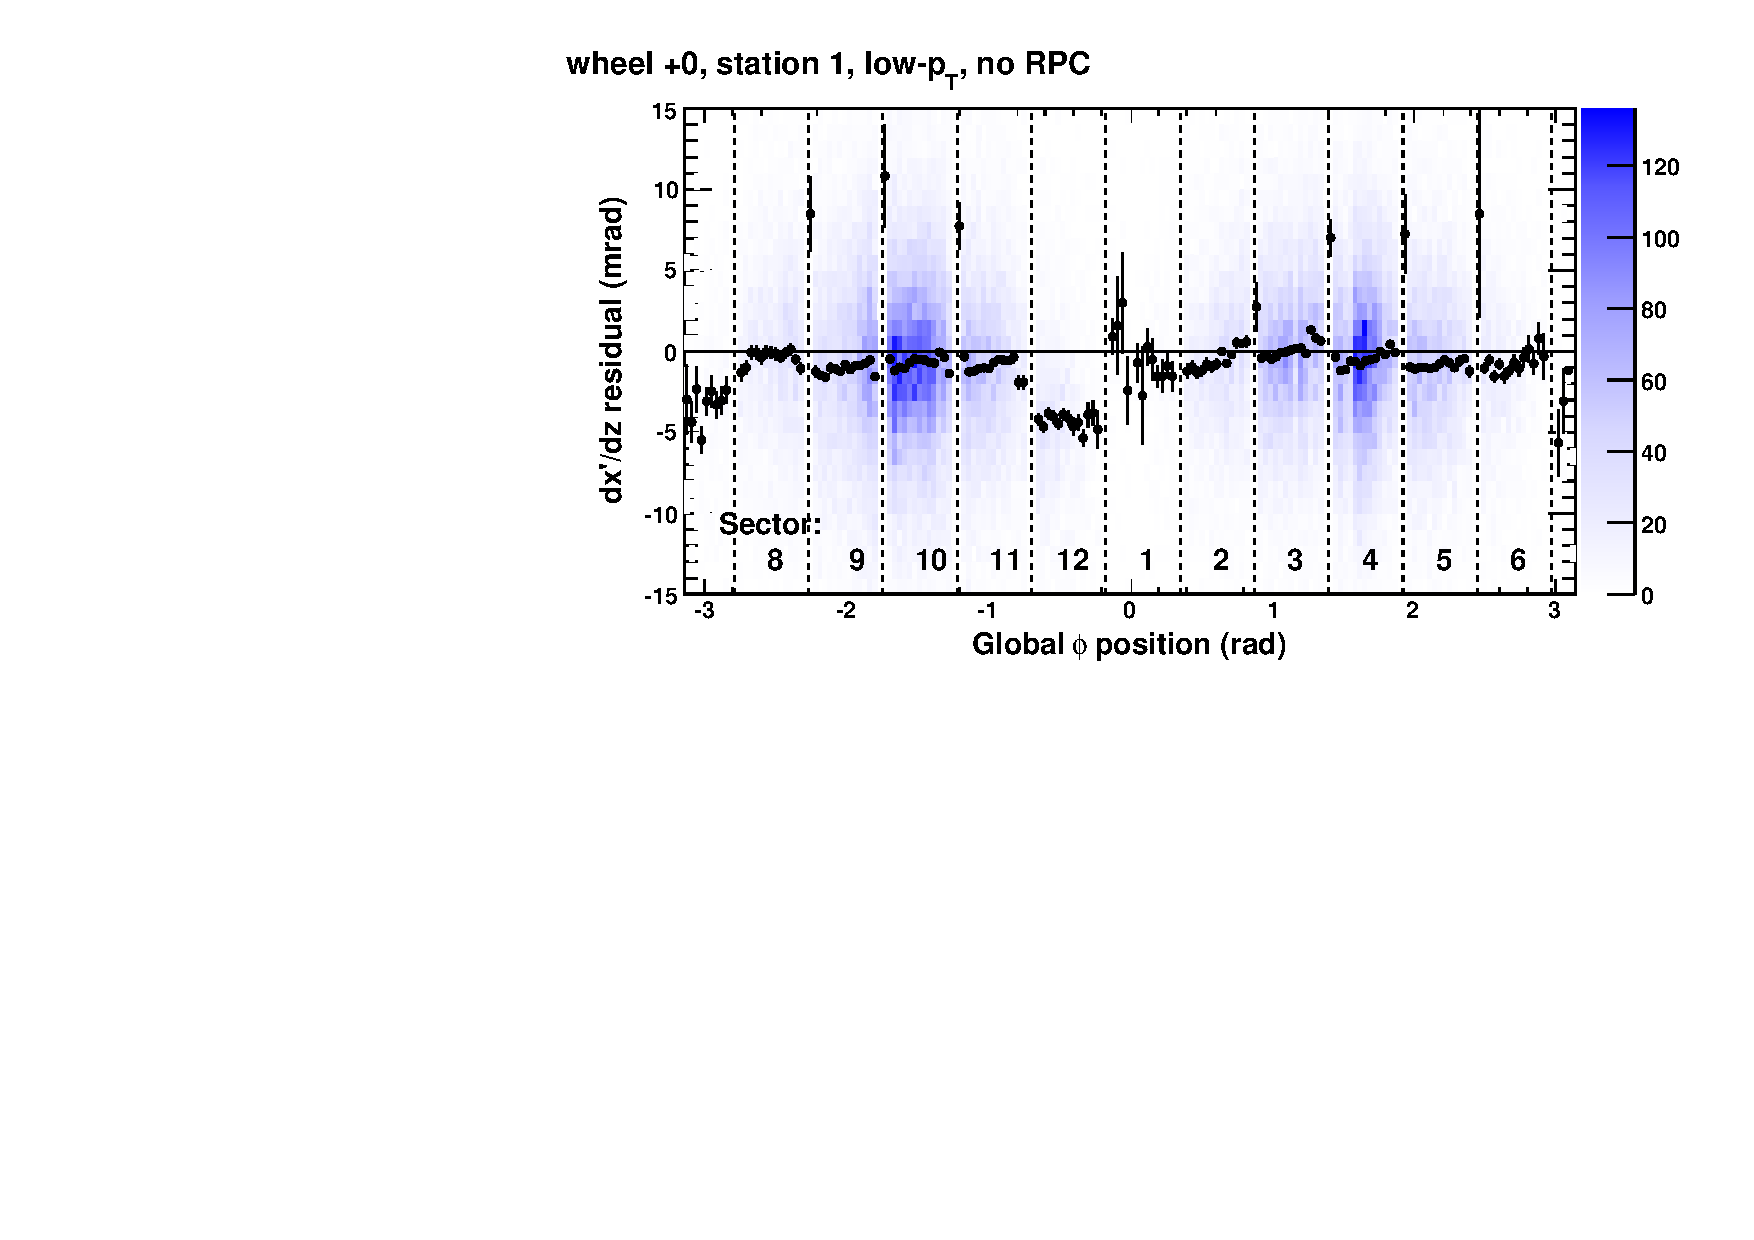
\includegraphics[width=\linewidth]{sawtoothexample_dxdz_low_norpc.pdf}}

\only<3>{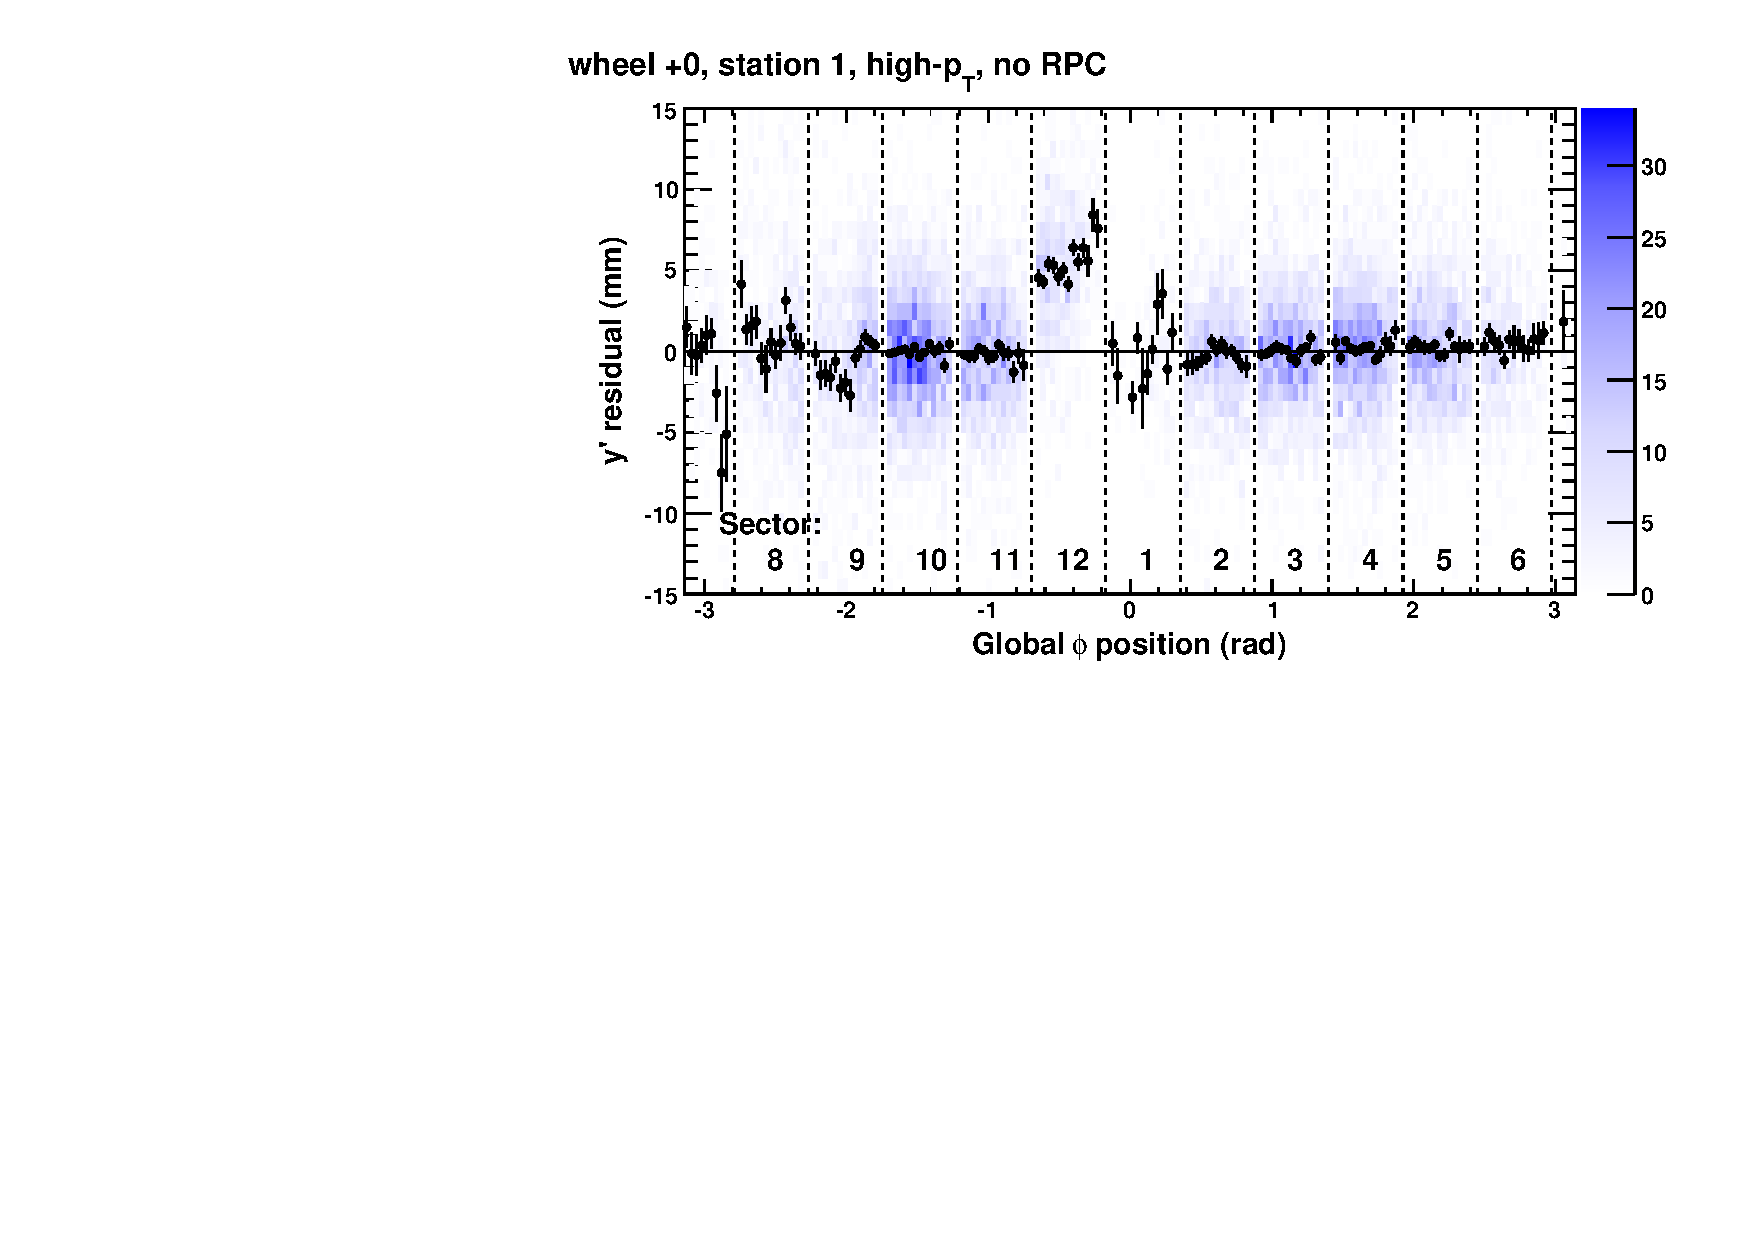
\includegraphics[width=\linewidth]{sawtoothexample_y_high_norpc.pdf}}

\only<3>{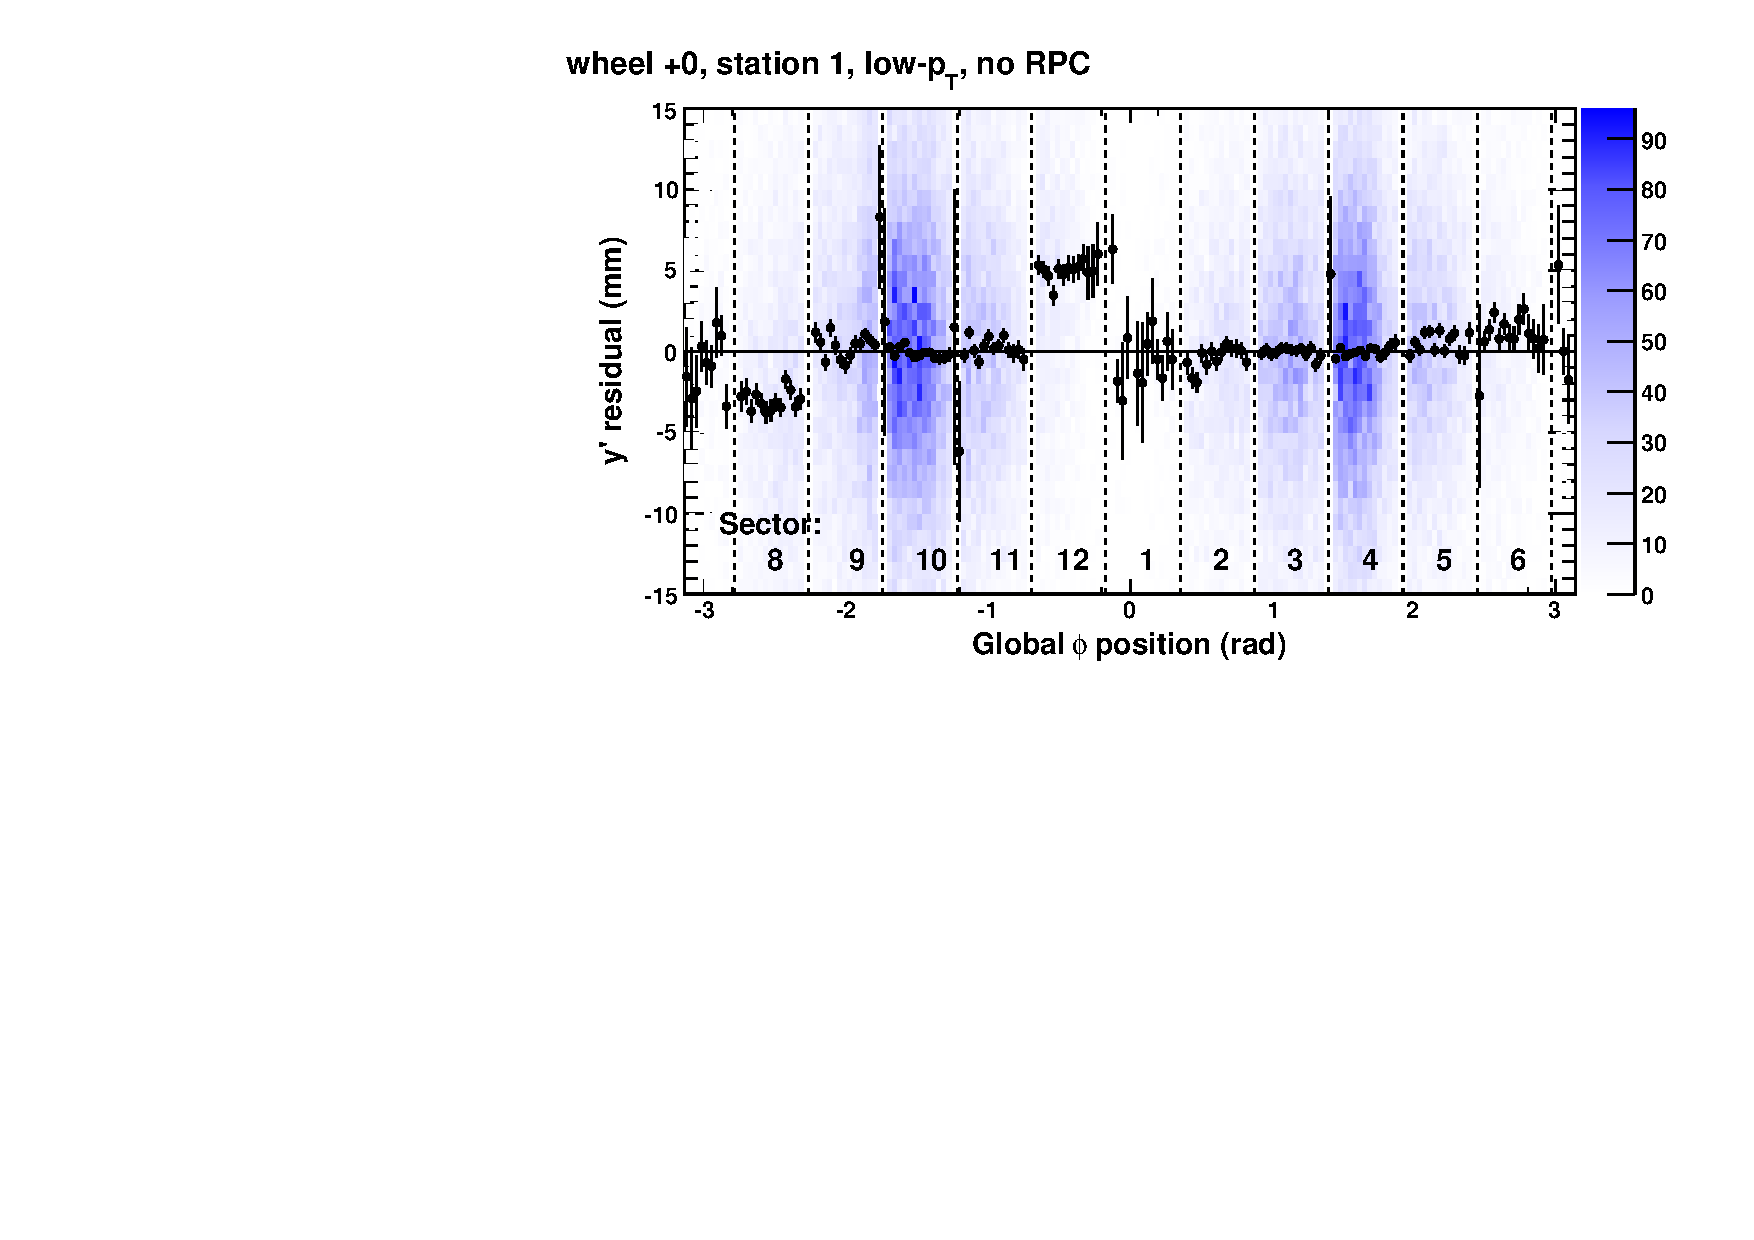
\includegraphics[width=\linewidth]{sawtoothexample_y_low_norpc.pdf}}

\only<4>{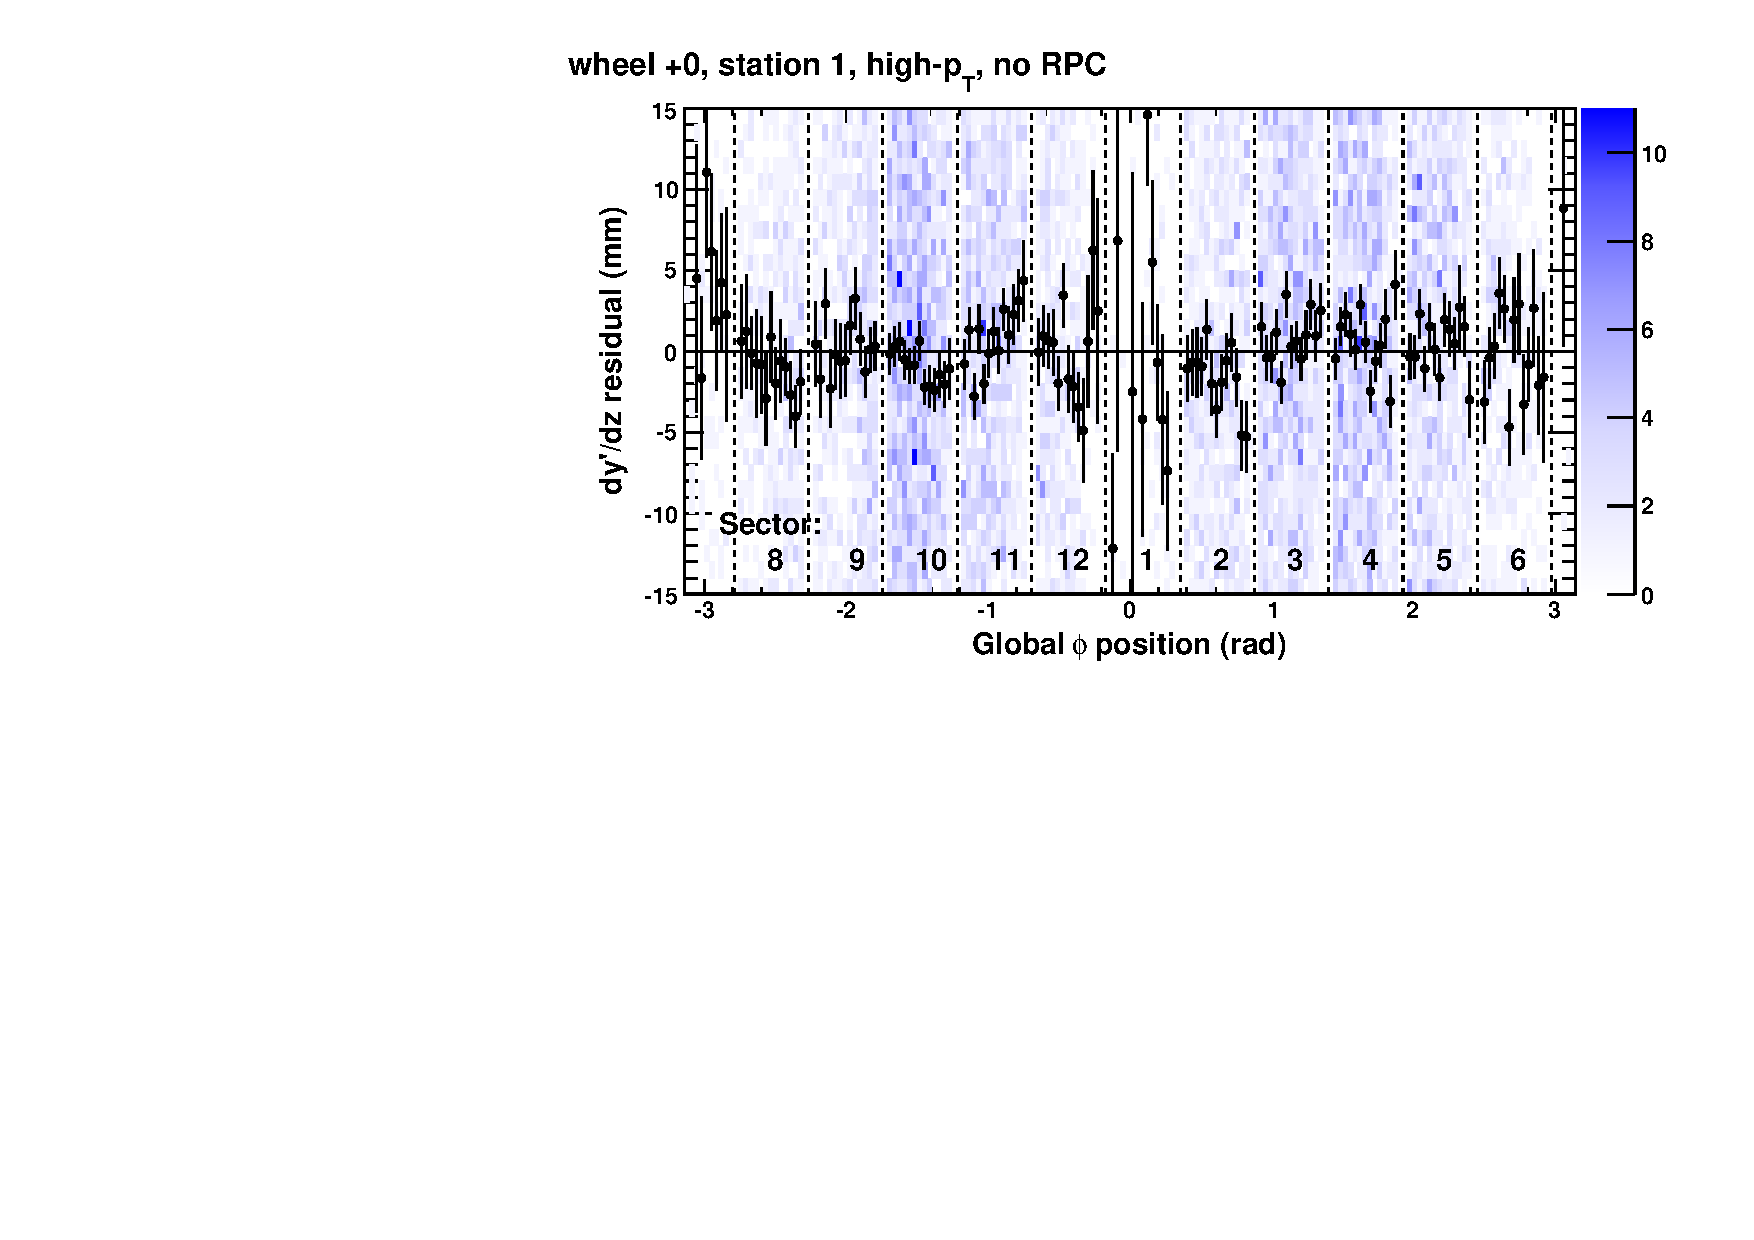
\includegraphics[width=\linewidth]{sawtoothexample_dydz_high_norpc.pdf}}

\only<4>{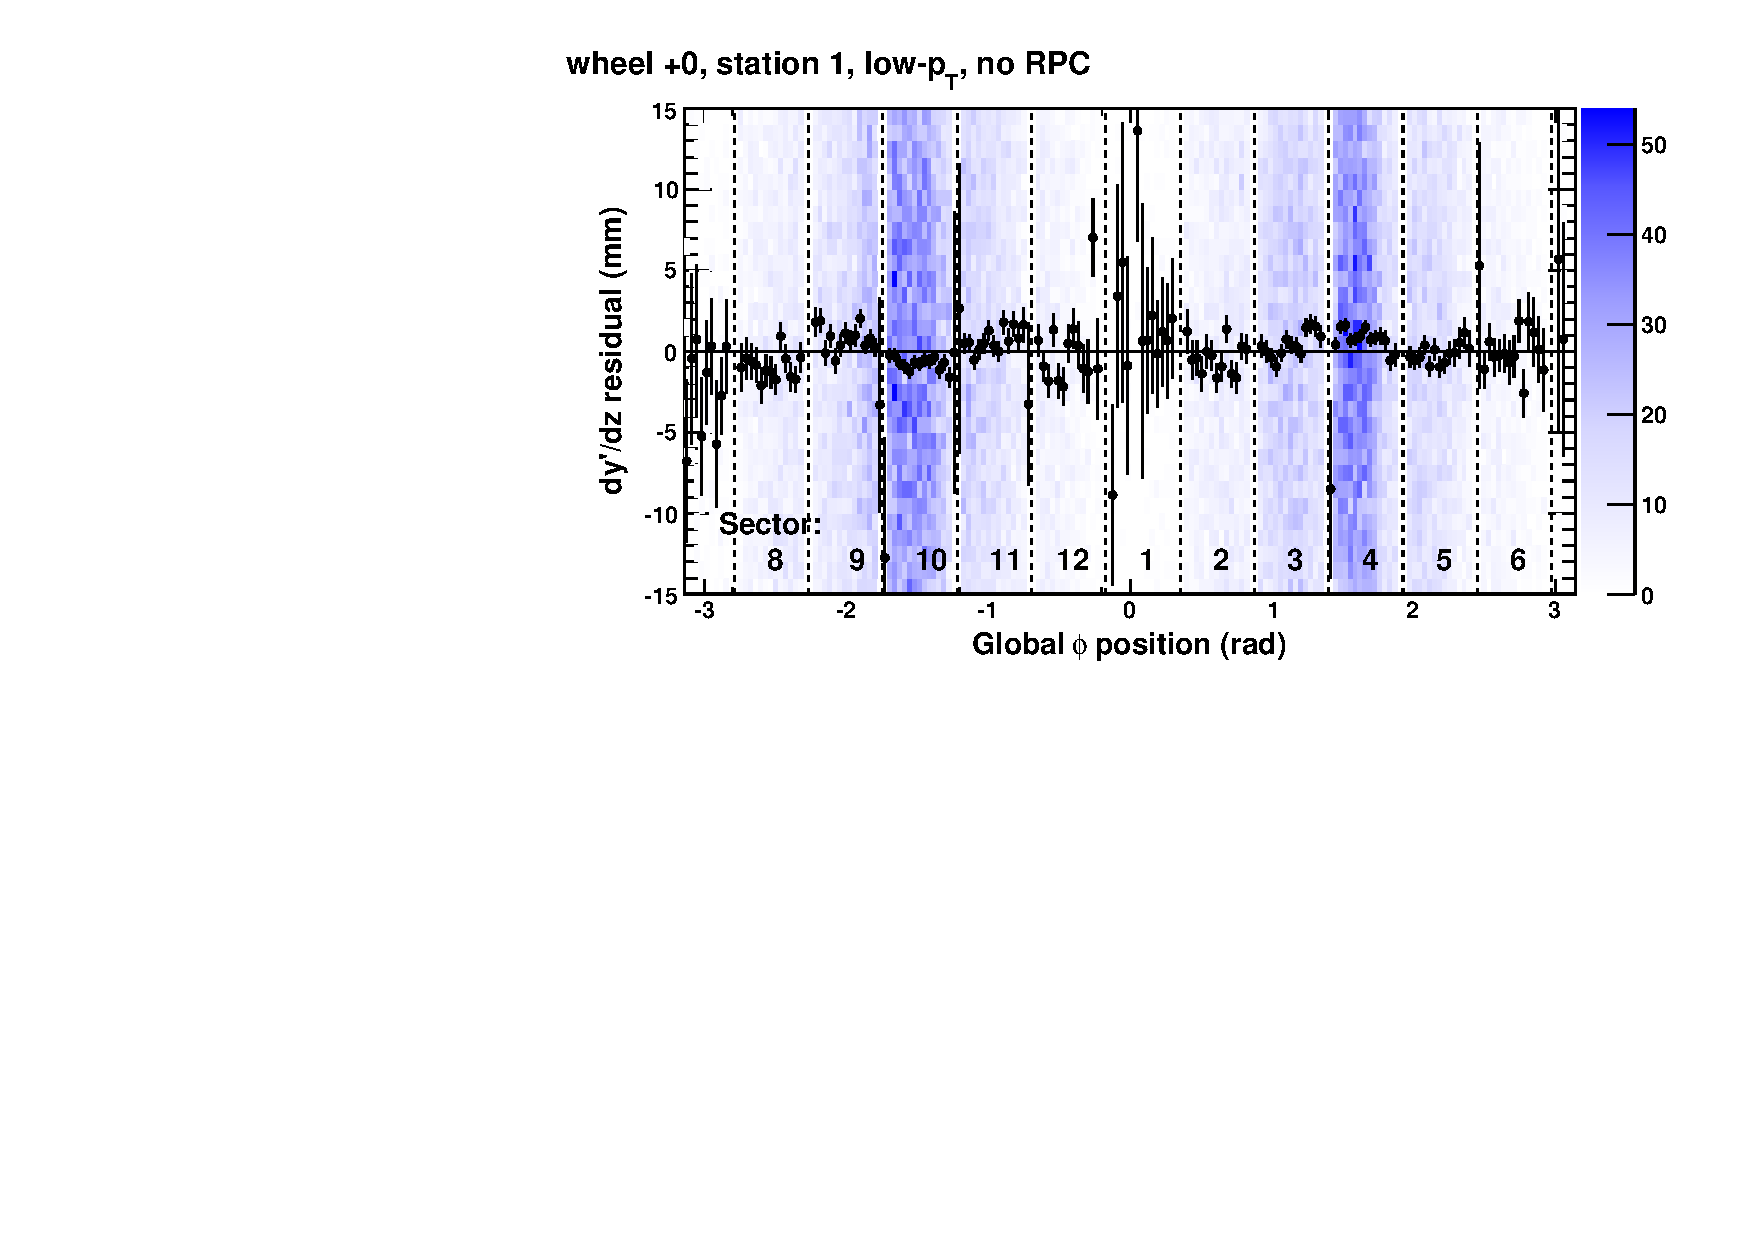
\includegraphics[width=\linewidth]{sawtoothexample_dydz_low_norpc.pdf}}

\end{columns}

\hfill \textcolor{darkblue}{\scriptsize CRAFT-09}
\end{frame}

\begin{frame}
\frametitle{Sawtooth (confirmation)}
\framesubtitle{``high-$p_T$'' means $p_T > 100$~GeV/$c$, ``low-$p_T$'' means $20 < p_T < 100$~GeV/$c$}

\vspace{-0.25 cm}
\begin{columns}
\column{0.28\linewidth}
\begin{center}
track refits biased by RPC hits
\end{center}
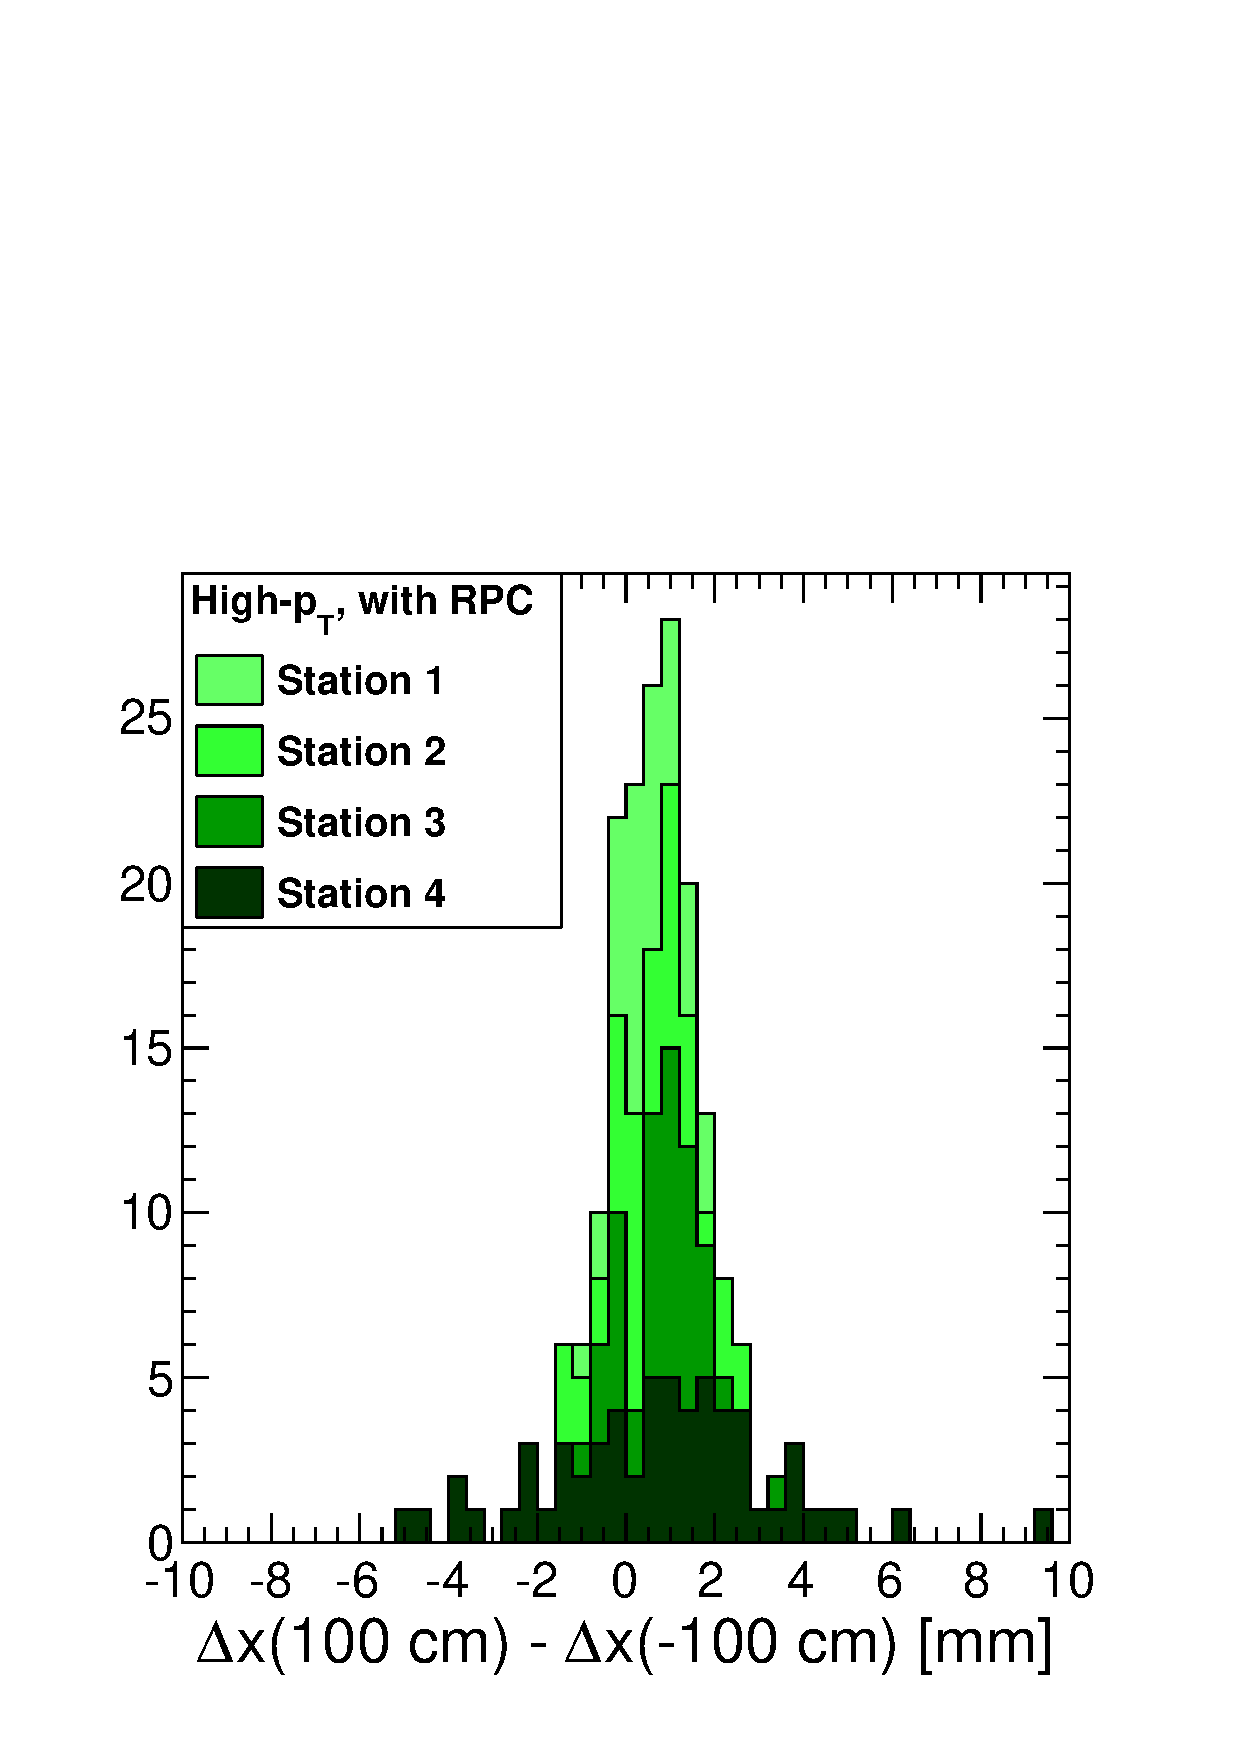
\includegraphics[width=\linewidth]{sawtooth_high_withrpc.pdf}

\fbox{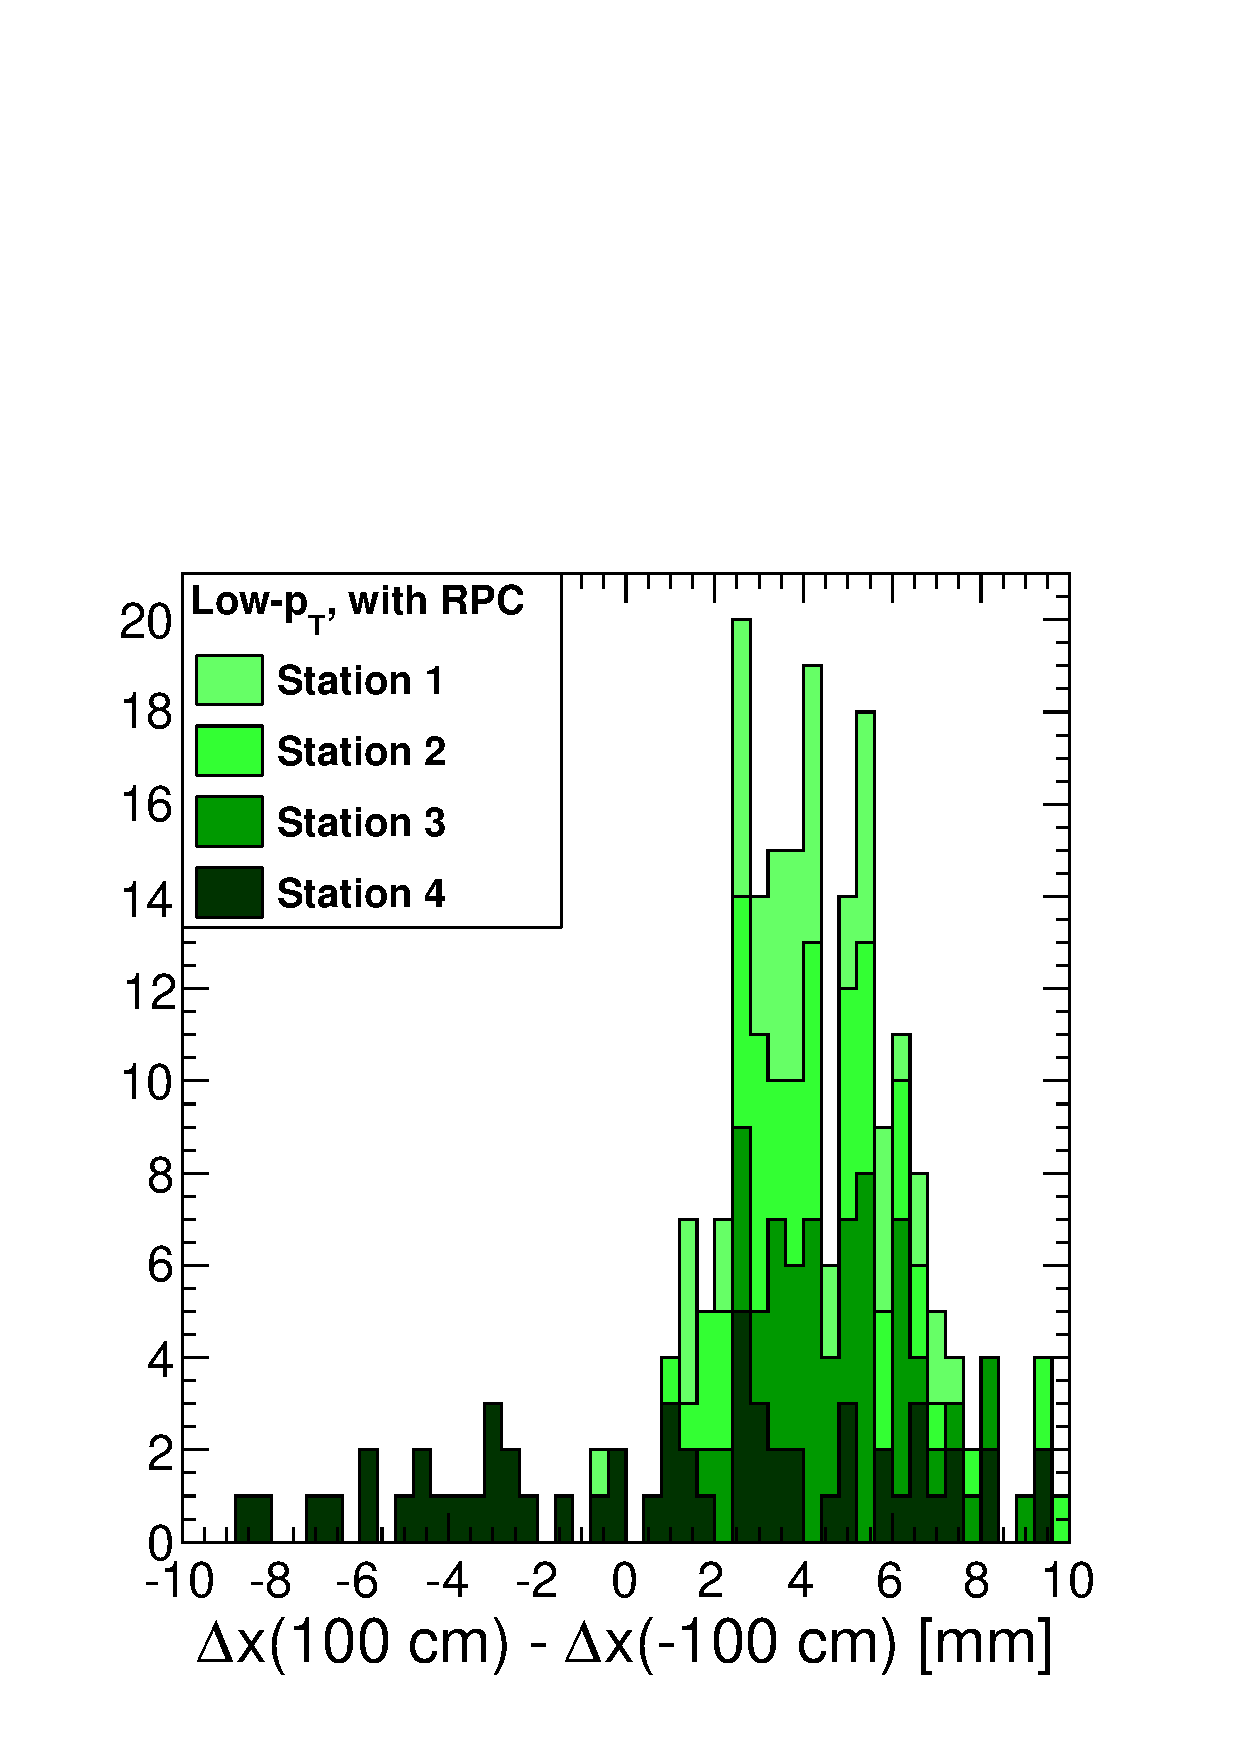
\includegraphics[width=\linewidth]{sawtooth_low_withrpc.pdf}}

\column{0.28\linewidth}
\begin{center}
unbiased track refits \\ \mbox{ }
\end{center}
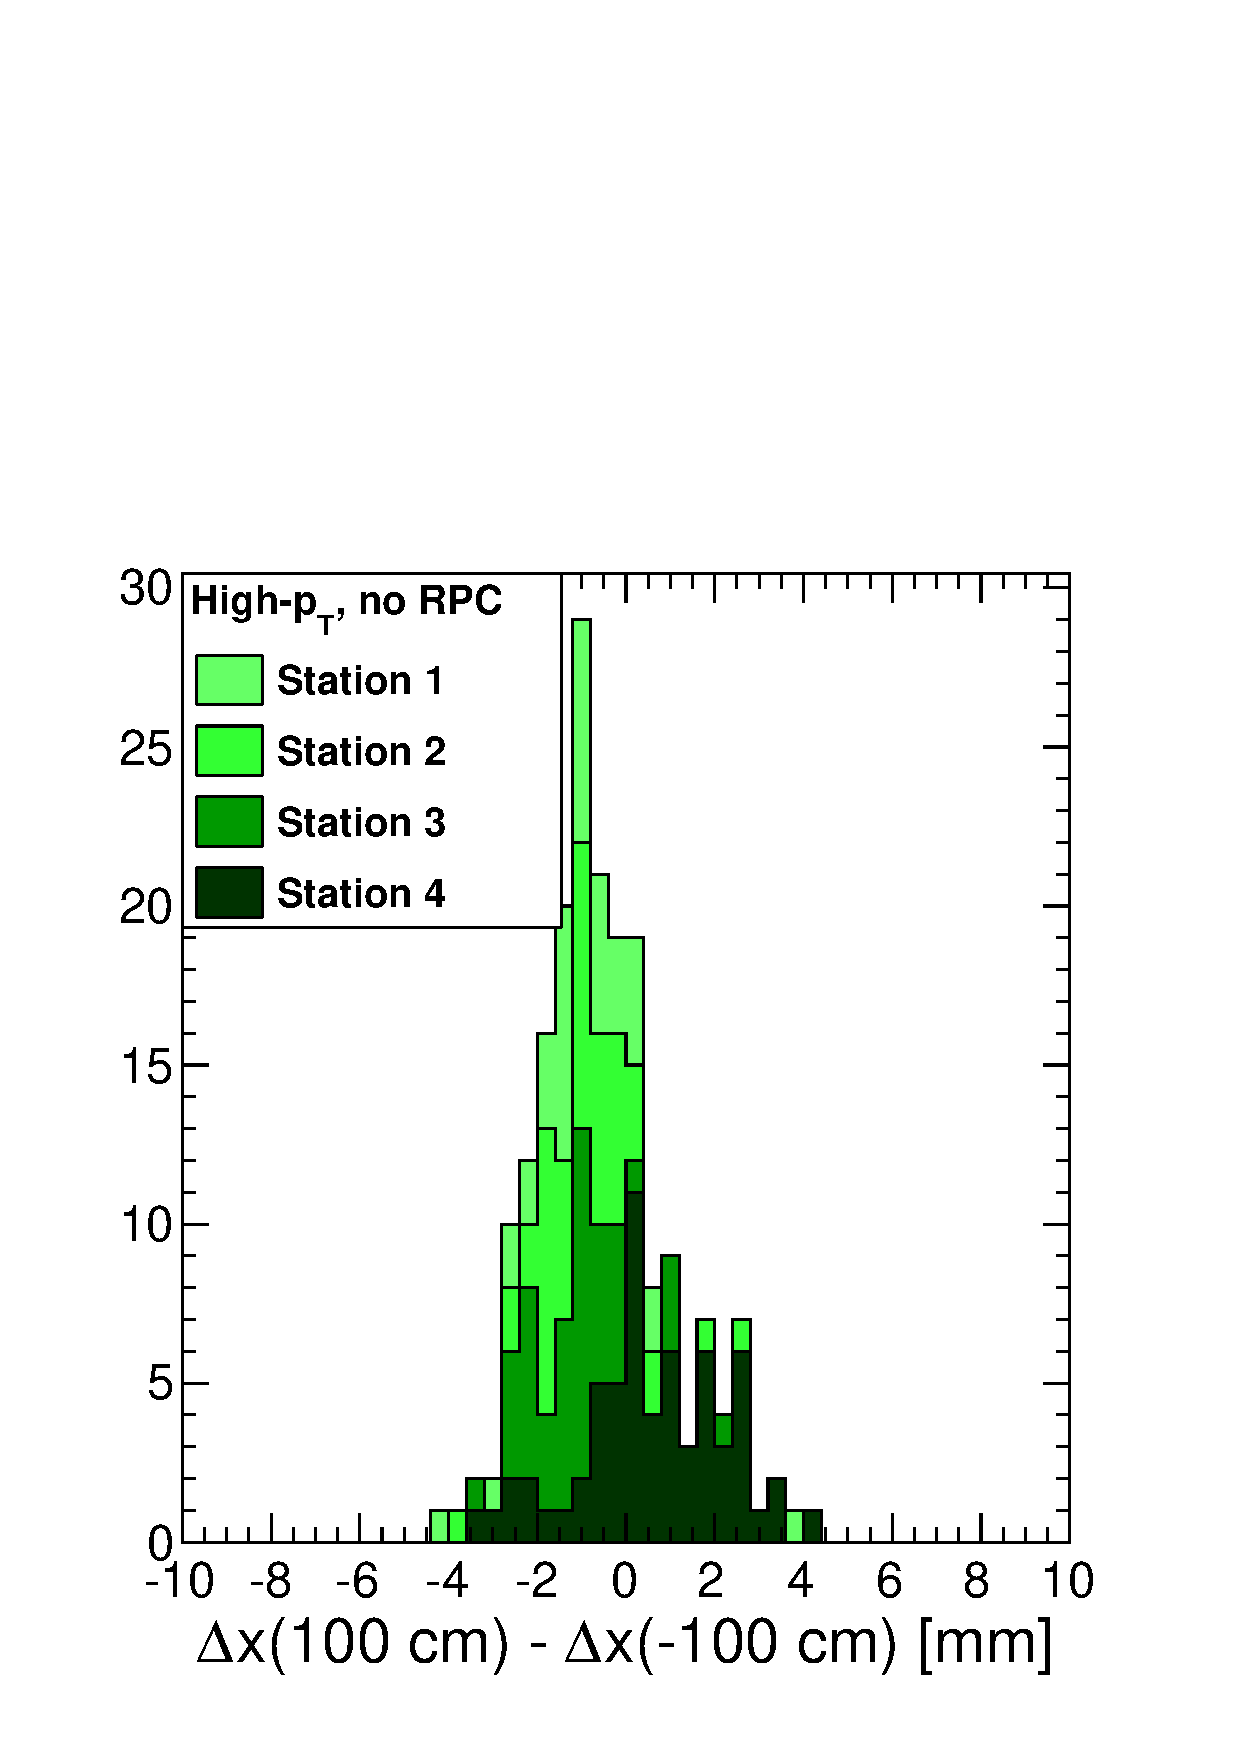
\includegraphics[width=\linewidth]{sawtooth_high_norpc.pdf}

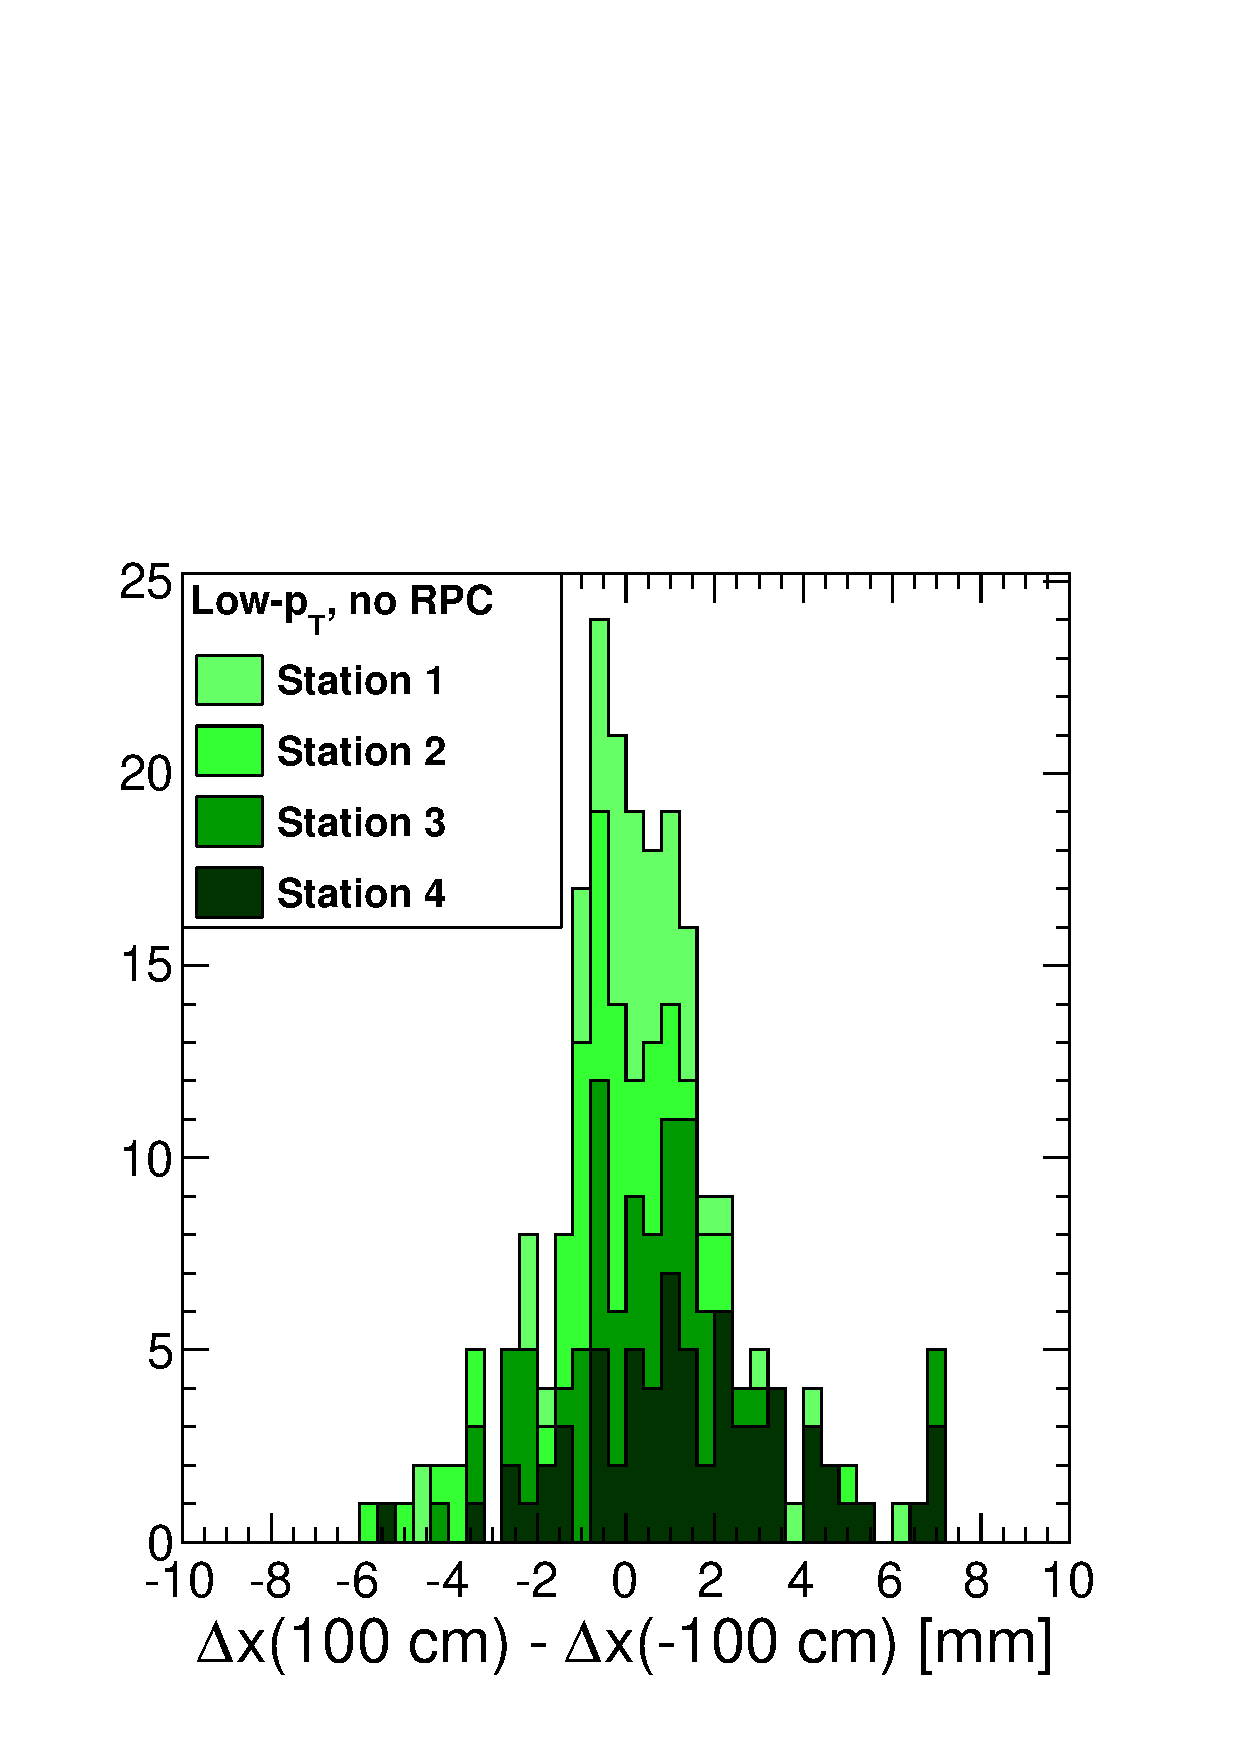
\includegraphics[width=\linewidth]{sawtooth_low_norpc.pdf}

\column{0.44\linewidth}
To make a summary plot:

\begin{enumerate}
\item Linear-fit to each chamber residual $\Delta x$ as a function of position $x$ (rough)

\item Express slopes of fits as $\Delta x$ at $x=+100$~cm minus
  $\Delta x$ at $x=-100$~cm \\ (size of ``tooth'' in sawtooth
  plot for a 200~cm chamber)

\item Make histograms of slopes
\end{enumerate}

\vspace{0.25 cm}
{\scriptsize (are there any RPCs in station~4?)}

\vspace{0.25 cm}
\hfill \textcolor{darkblue}{\scriptsize CRAFT-09}
\end{columns}
\end{frame}

\begin{frame}
\frametitle{Sawtooth in endcap (new)}

\vspace{-0.25 cm}
\begin{columns}
\column{0.5\linewidth}
\begin{itemize}
\item Aysen began studying CSC residuals from collisions globalMuons just two days ago
\item Saw strong sawtooth in ME1/2, but not elsewhere; \\ also eliminated with 
RefitRPCHits = False
\end{itemize}

\column{0.5\linewidth}
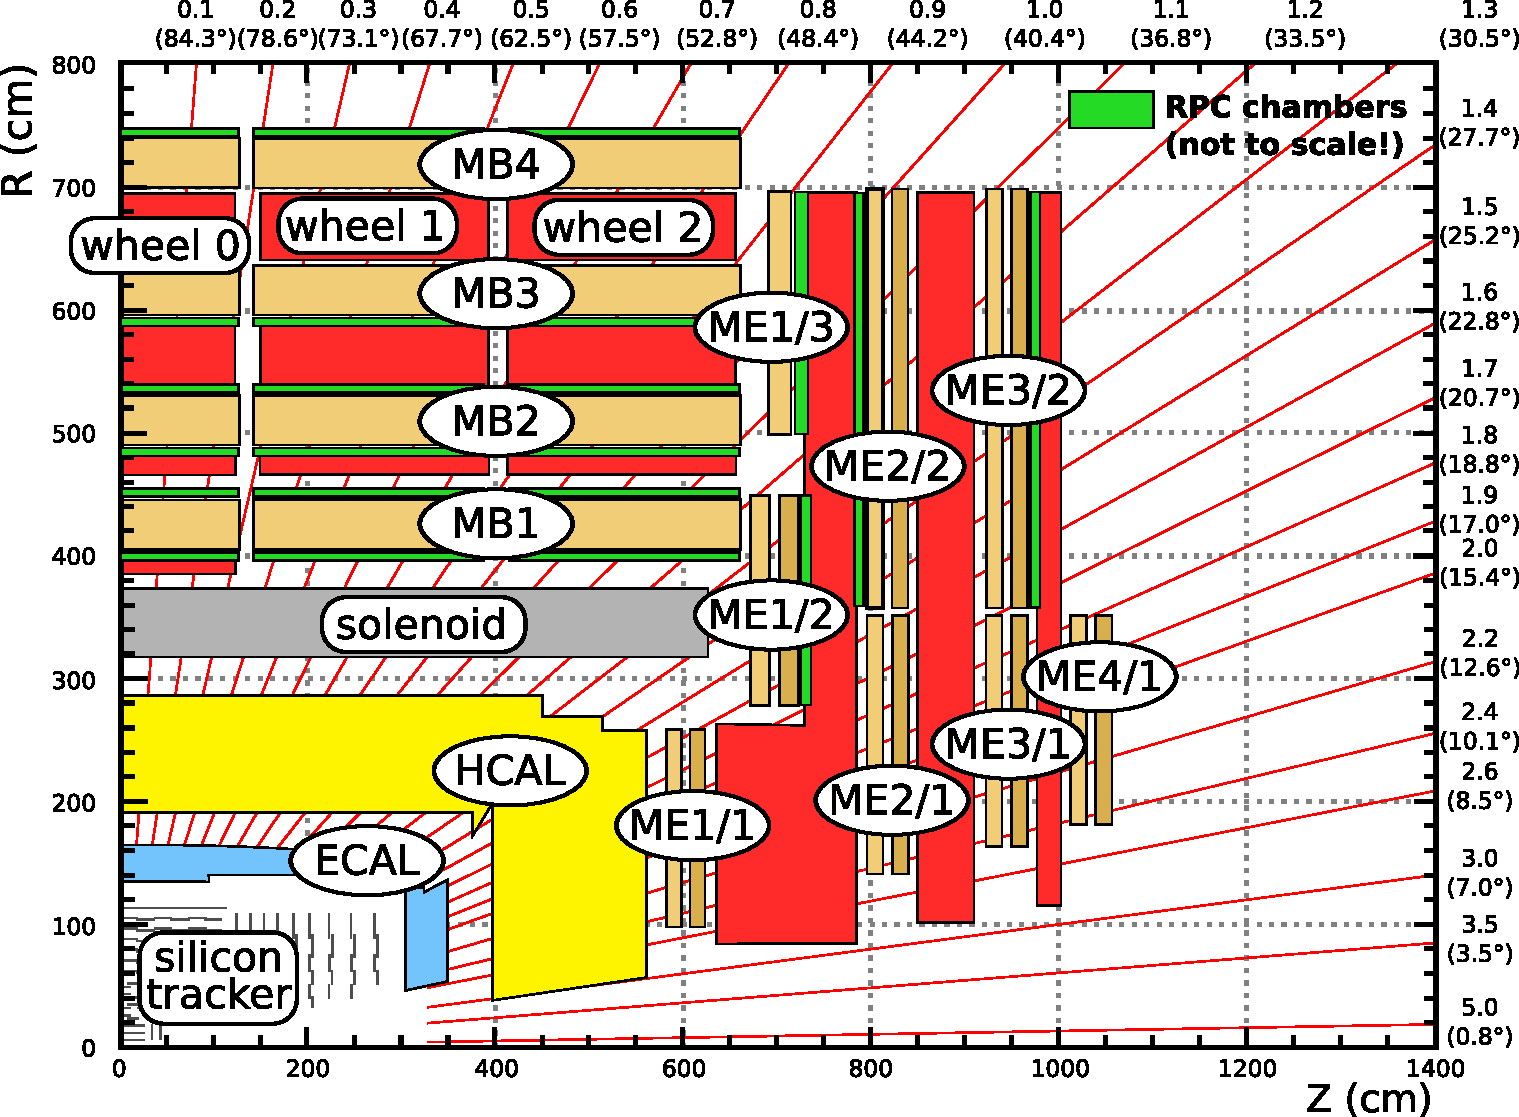
\includegraphics[width=\linewidth]{muon_system_withRPC.pdf}
\end{columns}

\vspace{0.25 cm}
\begin{columns}
\column{0.5\linewidth}
track refits biased by RPC hits

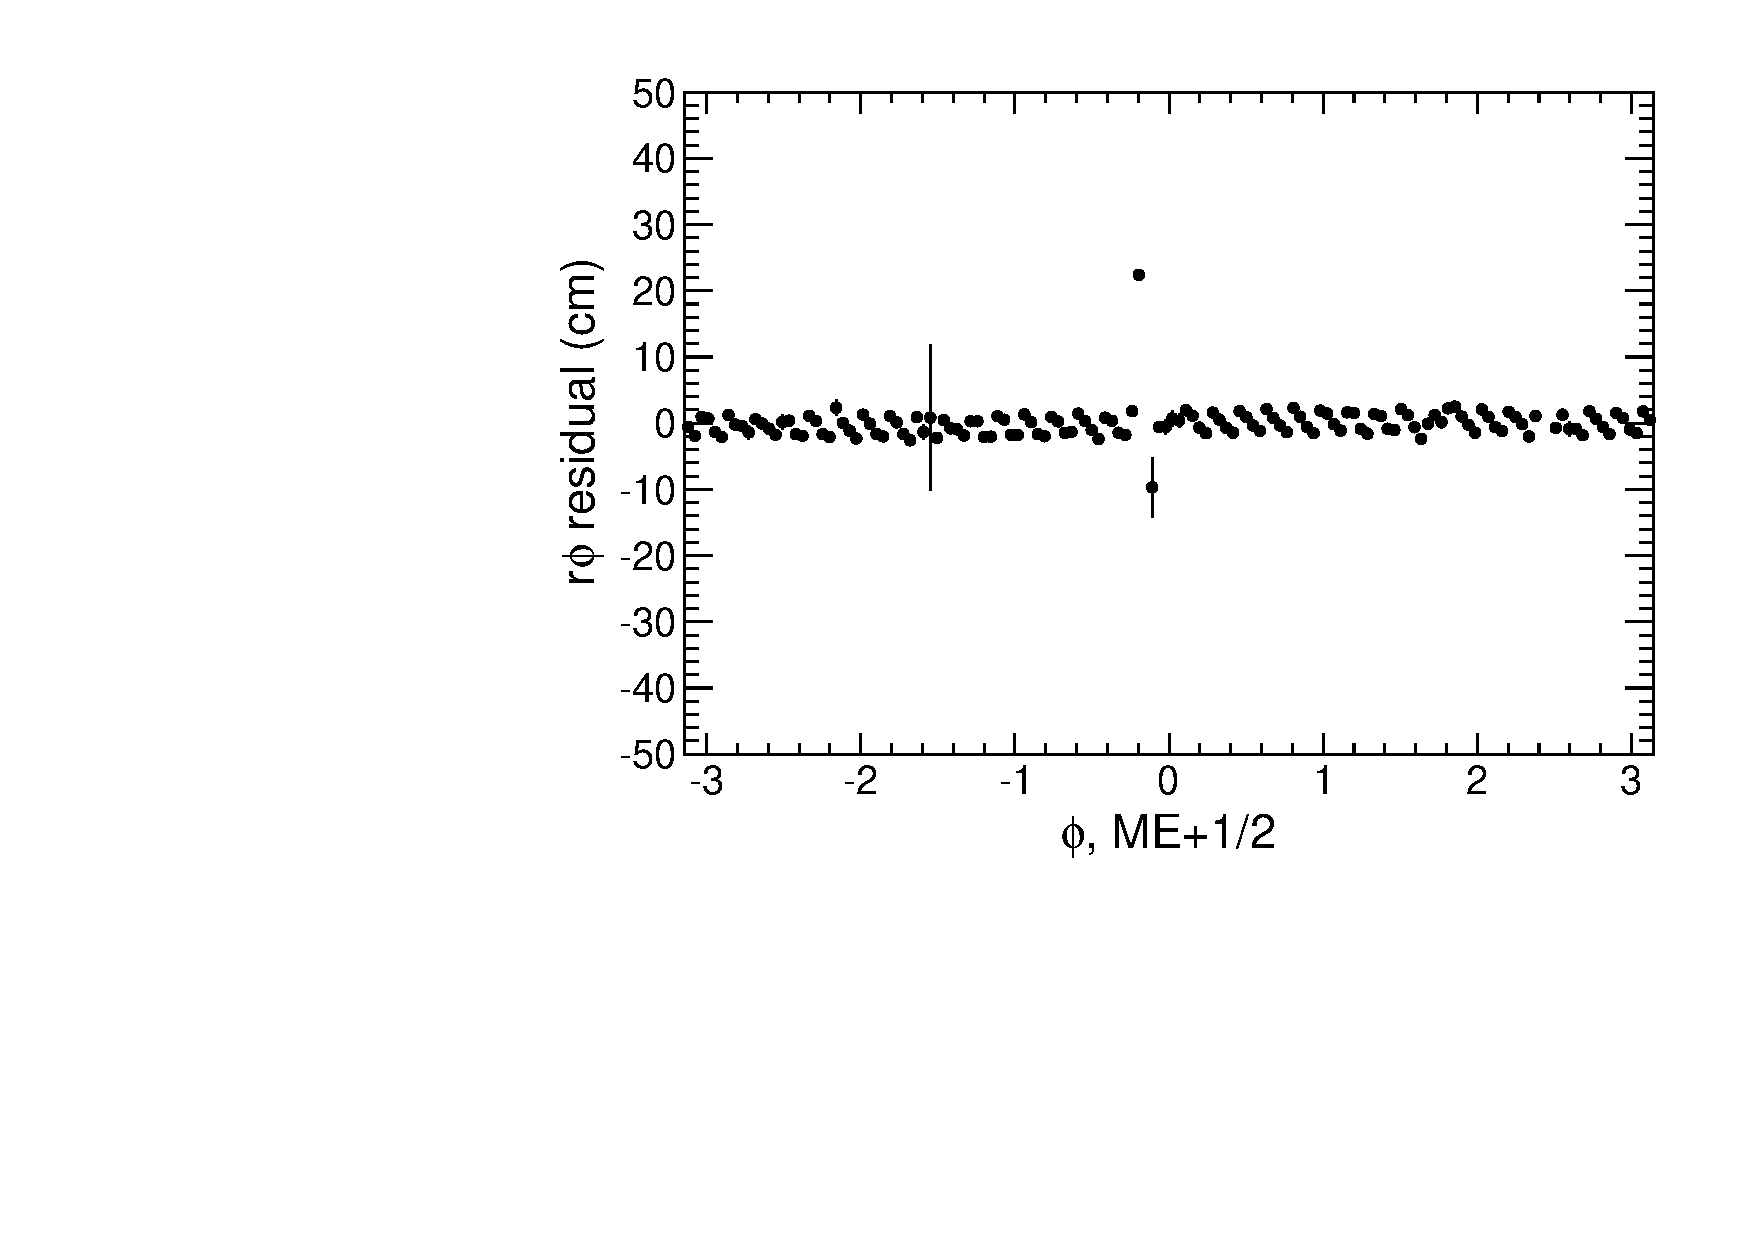
\includegraphics[width=\linewidth]{deltax_phi_prof_mep12_refitRPC.pdf}

\column{0.5\linewidth}
unbiased track refits

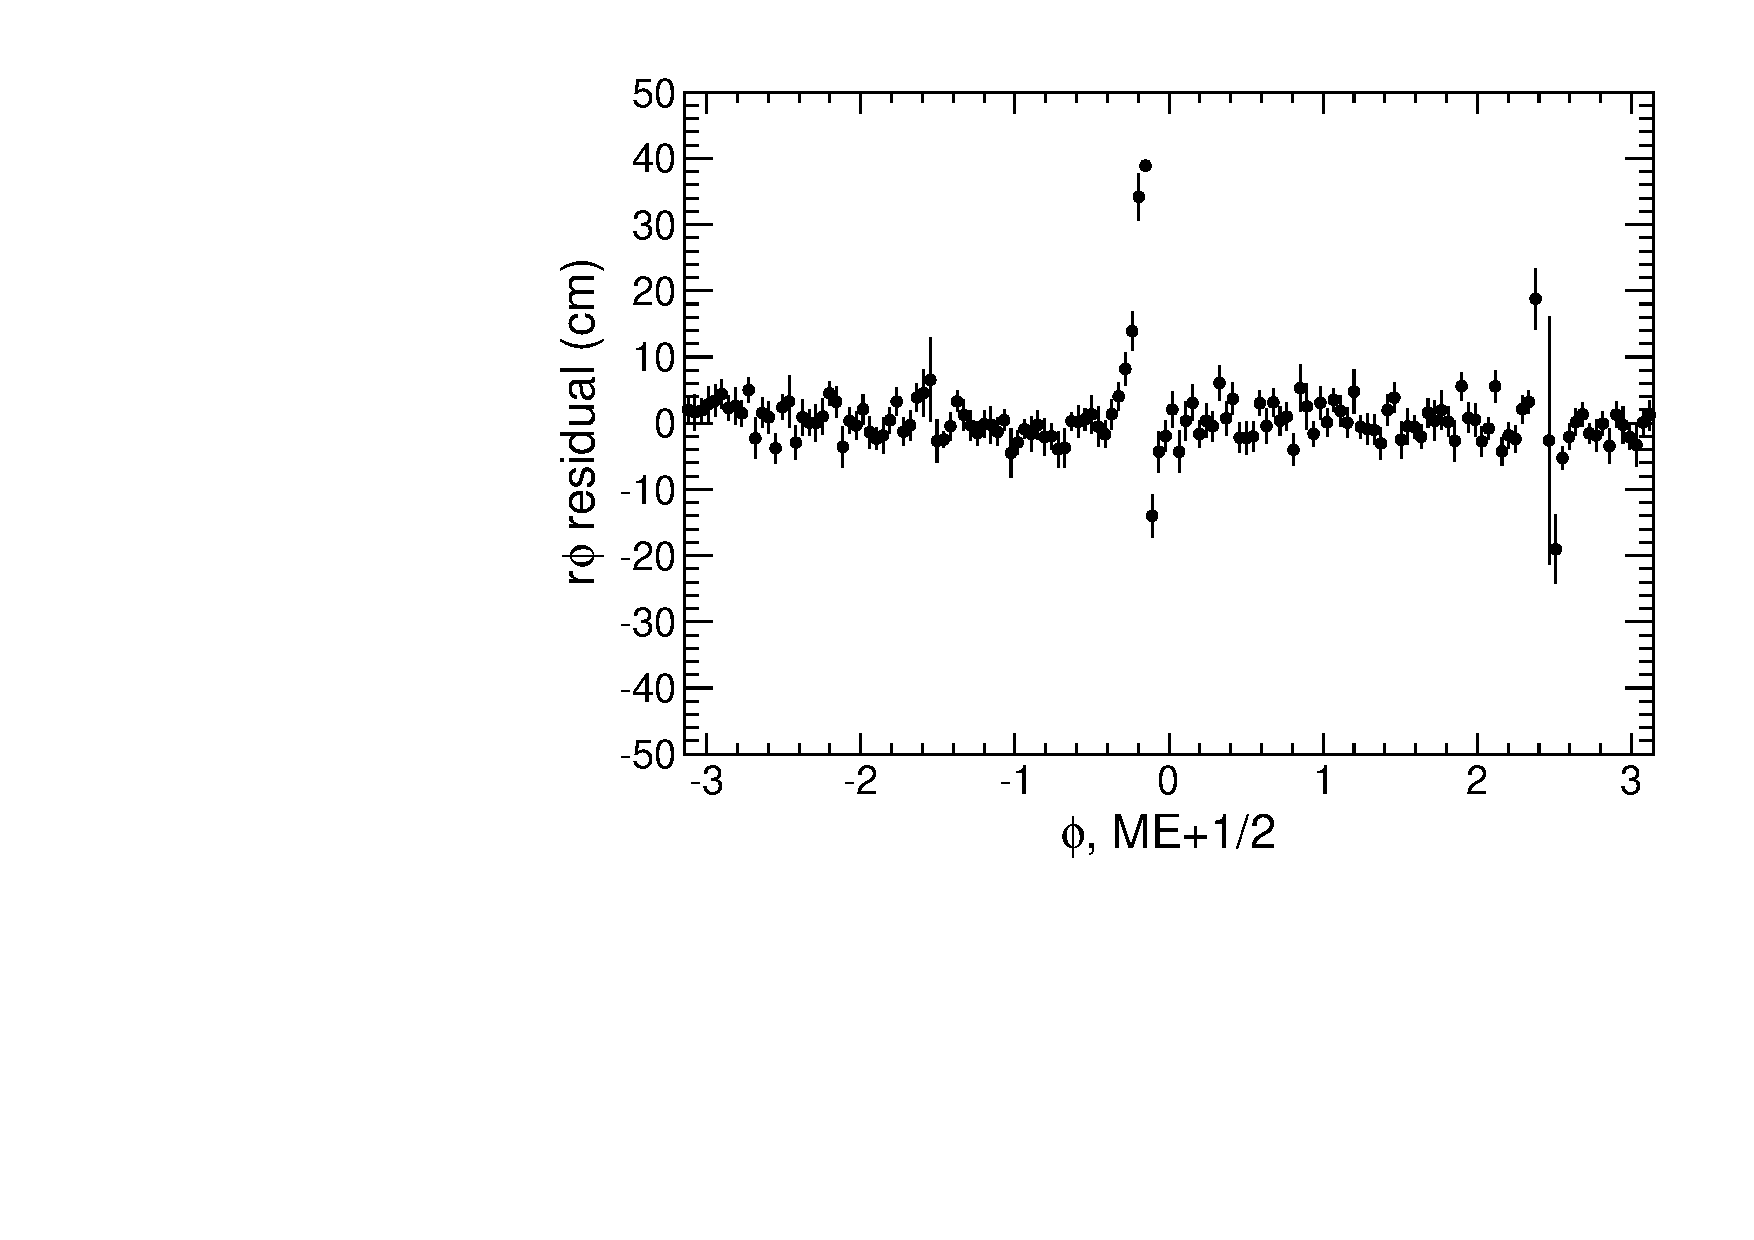
\includegraphics[width=\linewidth]{deltax_phi_prof_mep12_norefitRPC.pdf}
\end{columns}

\vspace{-1.25 cm}
\hfill \textcolor{darkblue}{\scriptsize 2010 collisions data}
\end{frame}

\begin{frame}
\frametitle{$q/p_T$ dependence (confirmation)}
\vspace{-0.6 cm}
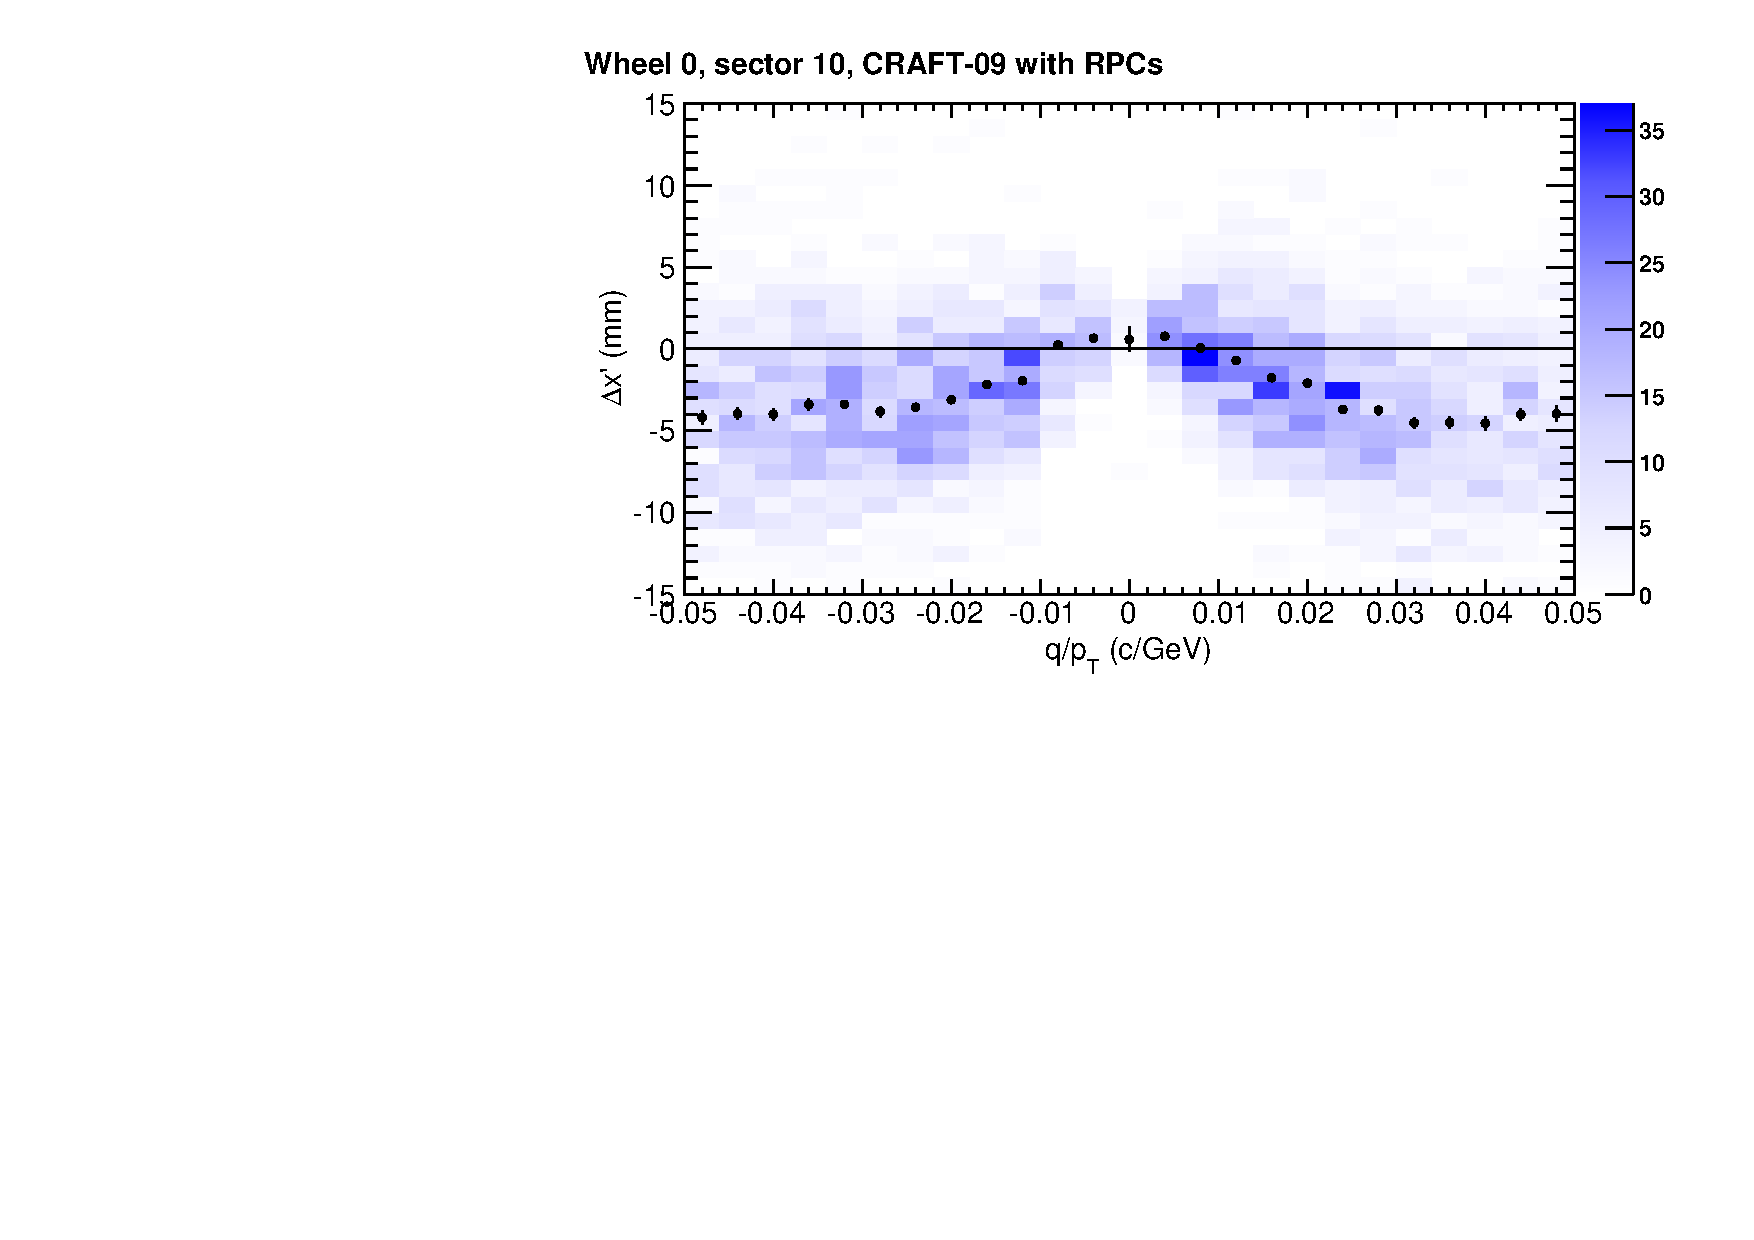
\includegraphics[width=0.5\linewidth]{globaldistort_withRPC.pdf}
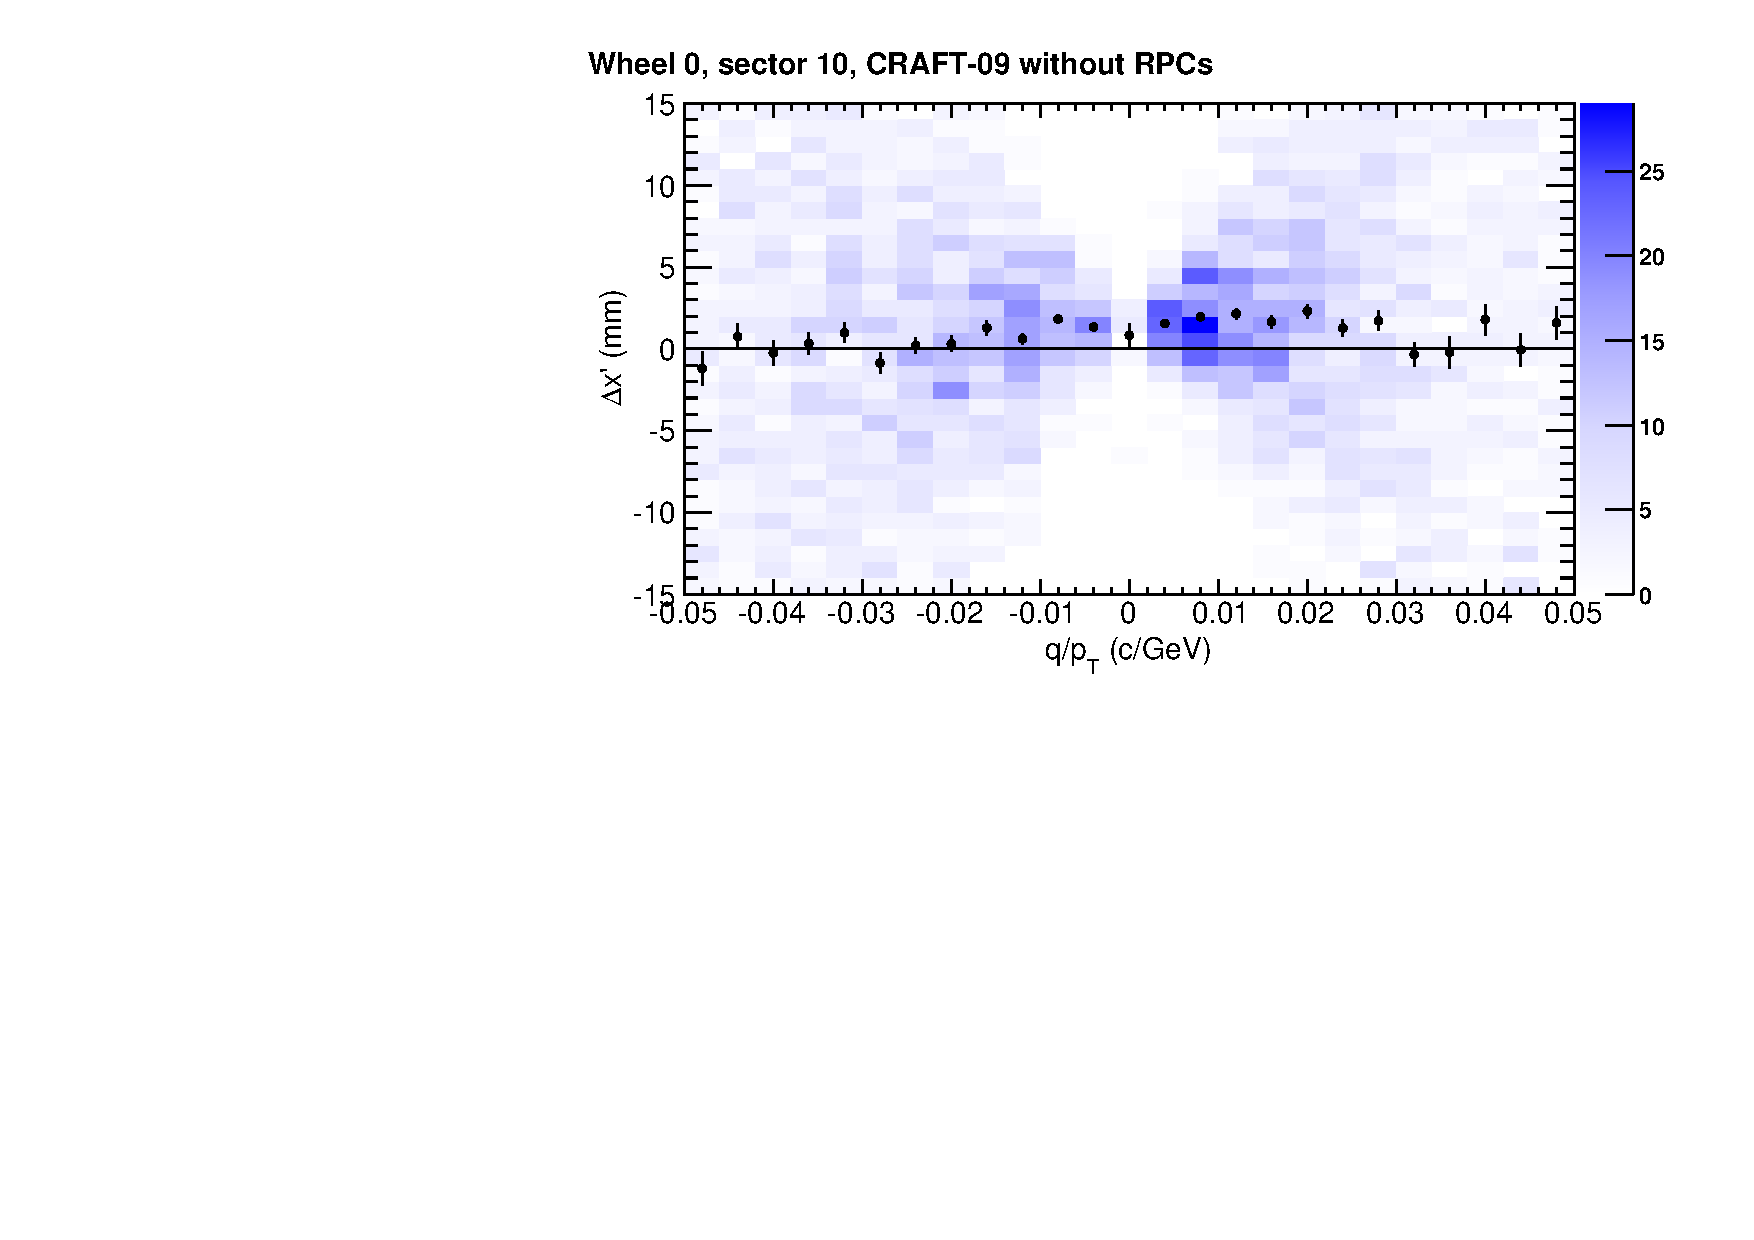
\includegraphics[width=0.5\linewidth]{globaldistort_noRPC.pdf}

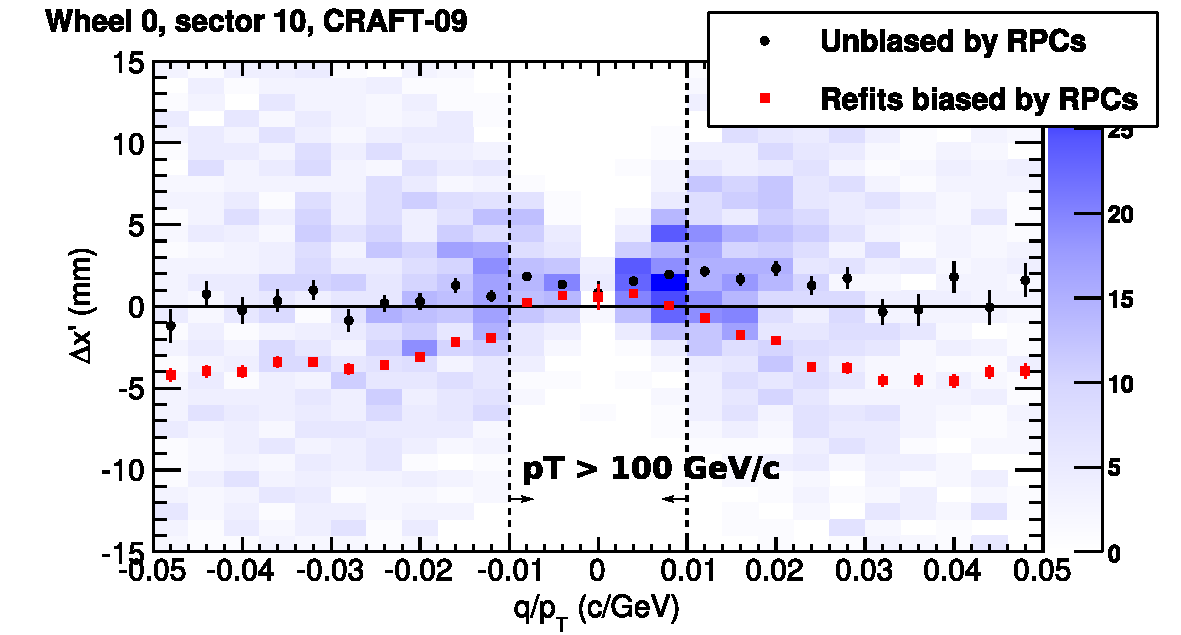
\includegraphics[width=\linewidth]{globaldistort_compare.pdf}

\vspace{-1.5 cm}
\hspace{0.93\linewidth} \textcolor{darkblue}{\mbox{\scriptsize CRAFT-09\hspace{-3 cm}}}
\end{frame}

\begin{frame}
\frametitle{Re-interpretation of this plot}

\begin{center}
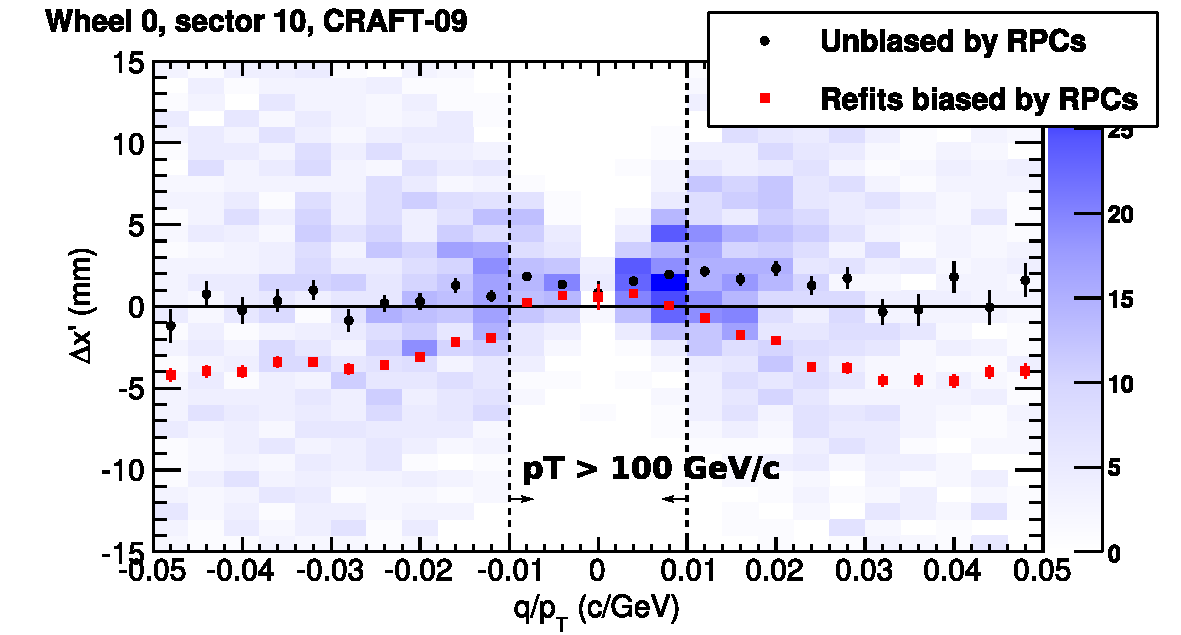
\includegraphics[width=0.75\linewidth]{globaldistort_compare.pdf}
\end{center}
\begin{itemize}
\item The ``100~GeV/$c$'' scale is set by RPC bias, not by tracker

\item Without RPC bias, there is no ``high-momentum
  vs.\ low-momentum'' discrepancy to explain: it's flat

\item The $p_T > 100$~GeV/$c$ cut limited impact of known but previously-unidentified bias

\item No significant linear slope: $\vec{B}$ appears to be okay
\end{itemize}

\vspace{-0.5 cm}
\hfill \textcolor{darkblue}{\scriptsize CRAFT-09}

\vspace{0.25 cm}
\end{frame}

\begin{frame}
\frametitle{$\vec{B}$-field study}

\begin{enumerate}
\item Fit all $\Delta x$ vs.\ $q/p_T$ plots in station~1 to straight lines
\item Plot all of the slopes (in cm $\cdot$ GeV/$c$)
\end{enumerate}

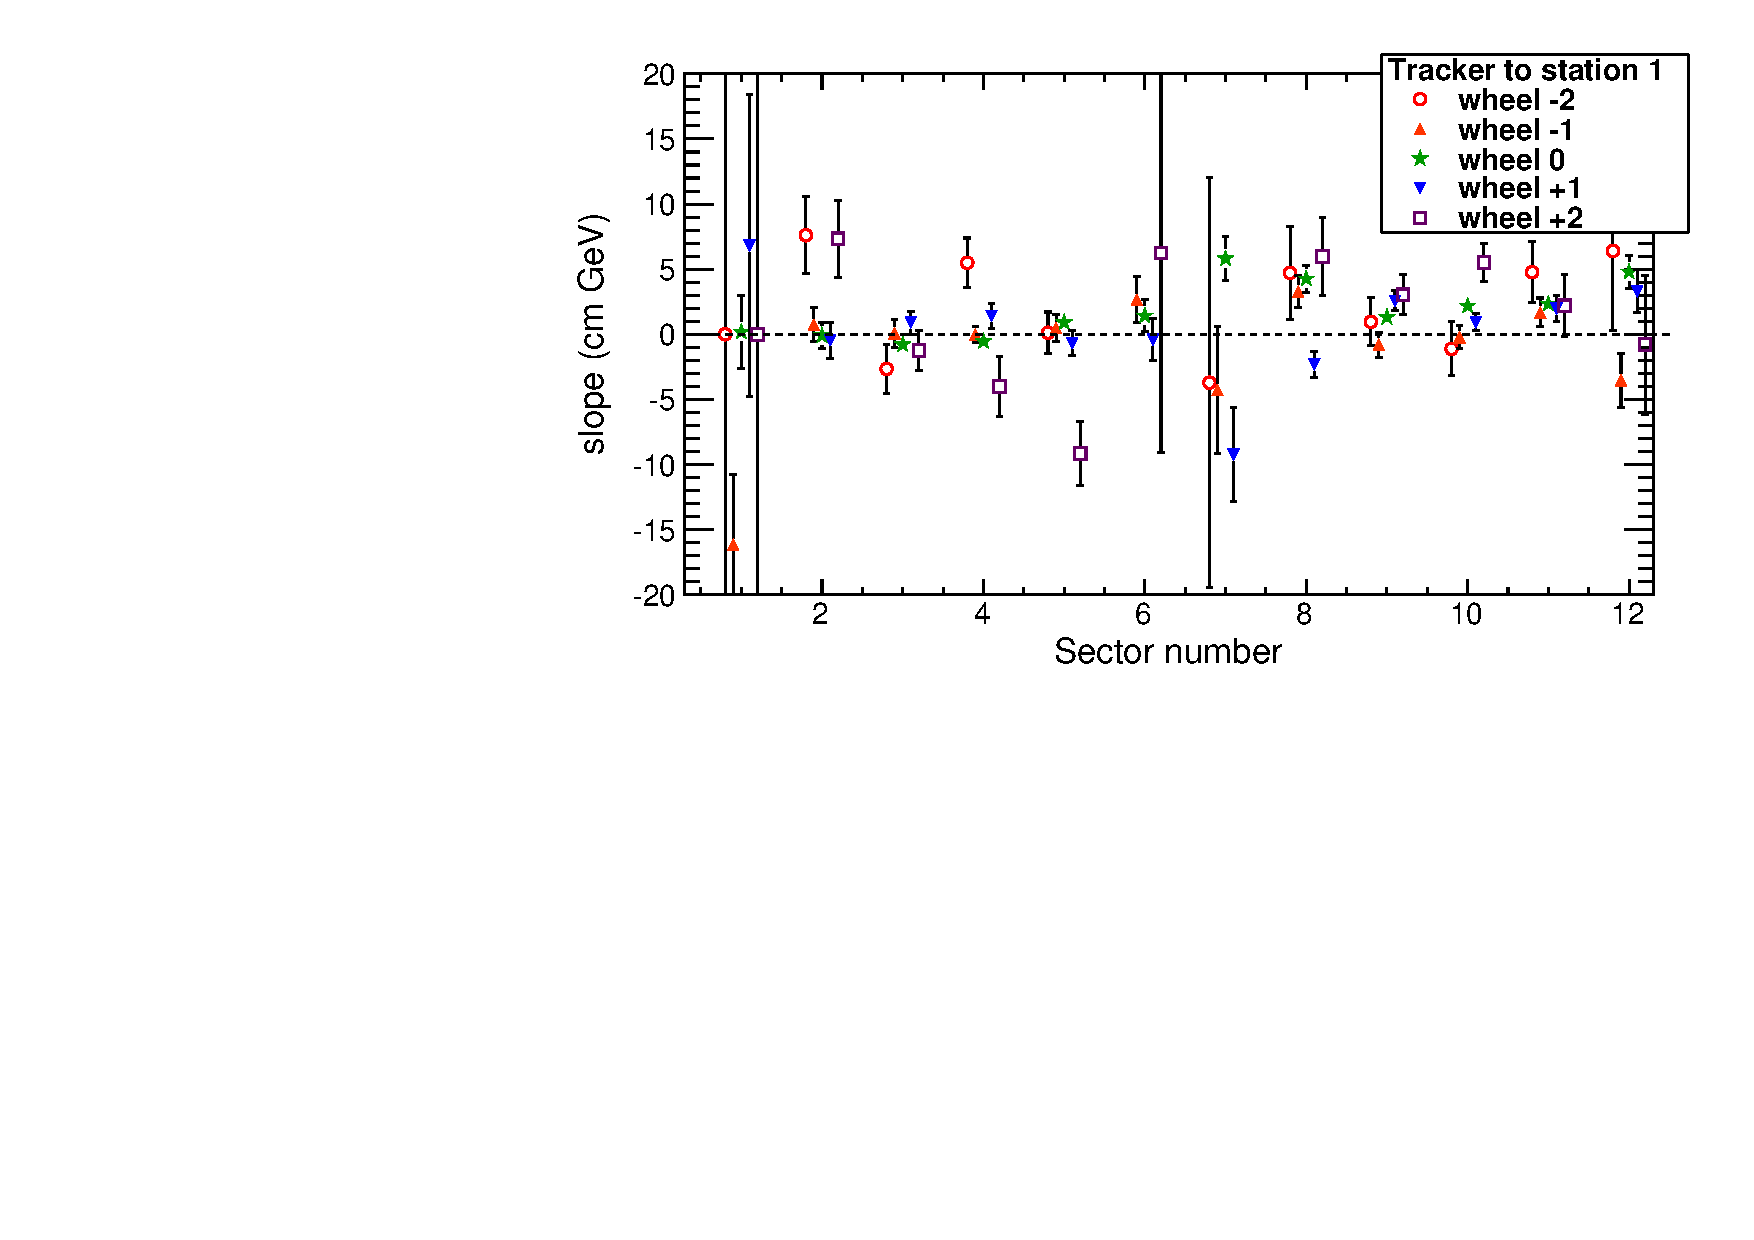
\includegraphics[width=\linewidth]{bfield_slopes.pdf}

\vspace{-0.5 cm}
\[ \hspace{-0.5 cm} \Delta x \cdot p_T = \frac{\ell^2}{2 (333~\mbox{cm})} 3.8~\mbox{T} \left(\frac{\Delta B}{B}\right) = \left\{\begin{array}{l l} 10~\mbox{cm} & \mbox{\scriptsize for $\ell$ = 400~cm} \\ 5~\mbox{cm} & \mbox{\scriptsize for $\ell$ = 300~cm} \end{array} \right. \mbox{ and } \frac{\Delta B}{B} = 1\% \]

\vspace{-0.25 cm}
\hfill \textcolor{darkblue}{\scriptsize CRAFT-09}

\vspace{0.25 cm}
\end{frame}

\begin{frame}
\frametitle{$\vec{B}$-field study}

\begin{itemize}
\item Same for differences in residuals between stations \only<1>{1 and 2}\only<2>{2 and 3}\only<3>{3 and 4}
\item Quantifies $\vec{B}$-field between stations \only<1>{1 and 2}\only<2>{2 and 3}\only<3>{3 and 4}: $\sim$10\% level
\end{itemize}

\only<1>{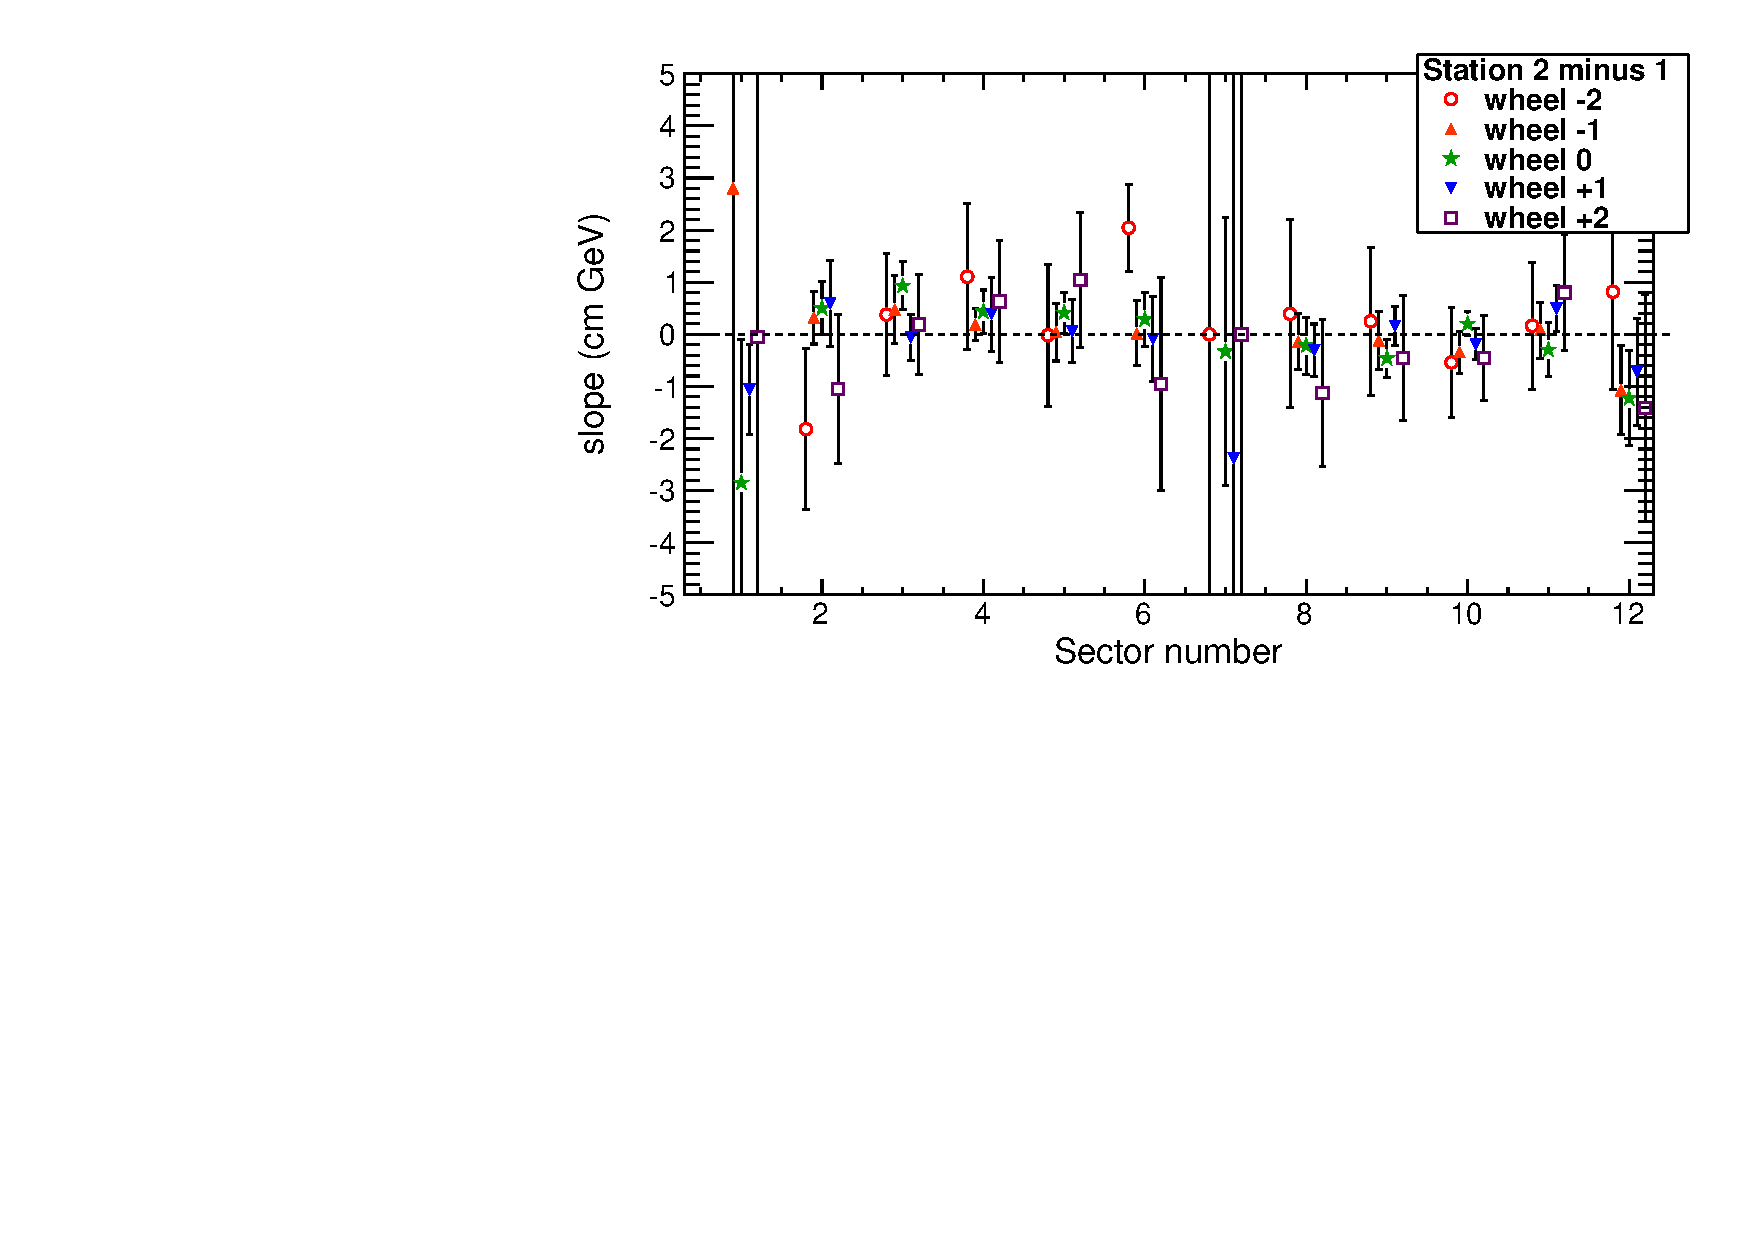
\includegraphics[width=\linewidth]{bfield_slopes_12.pdf}}
\only<2>{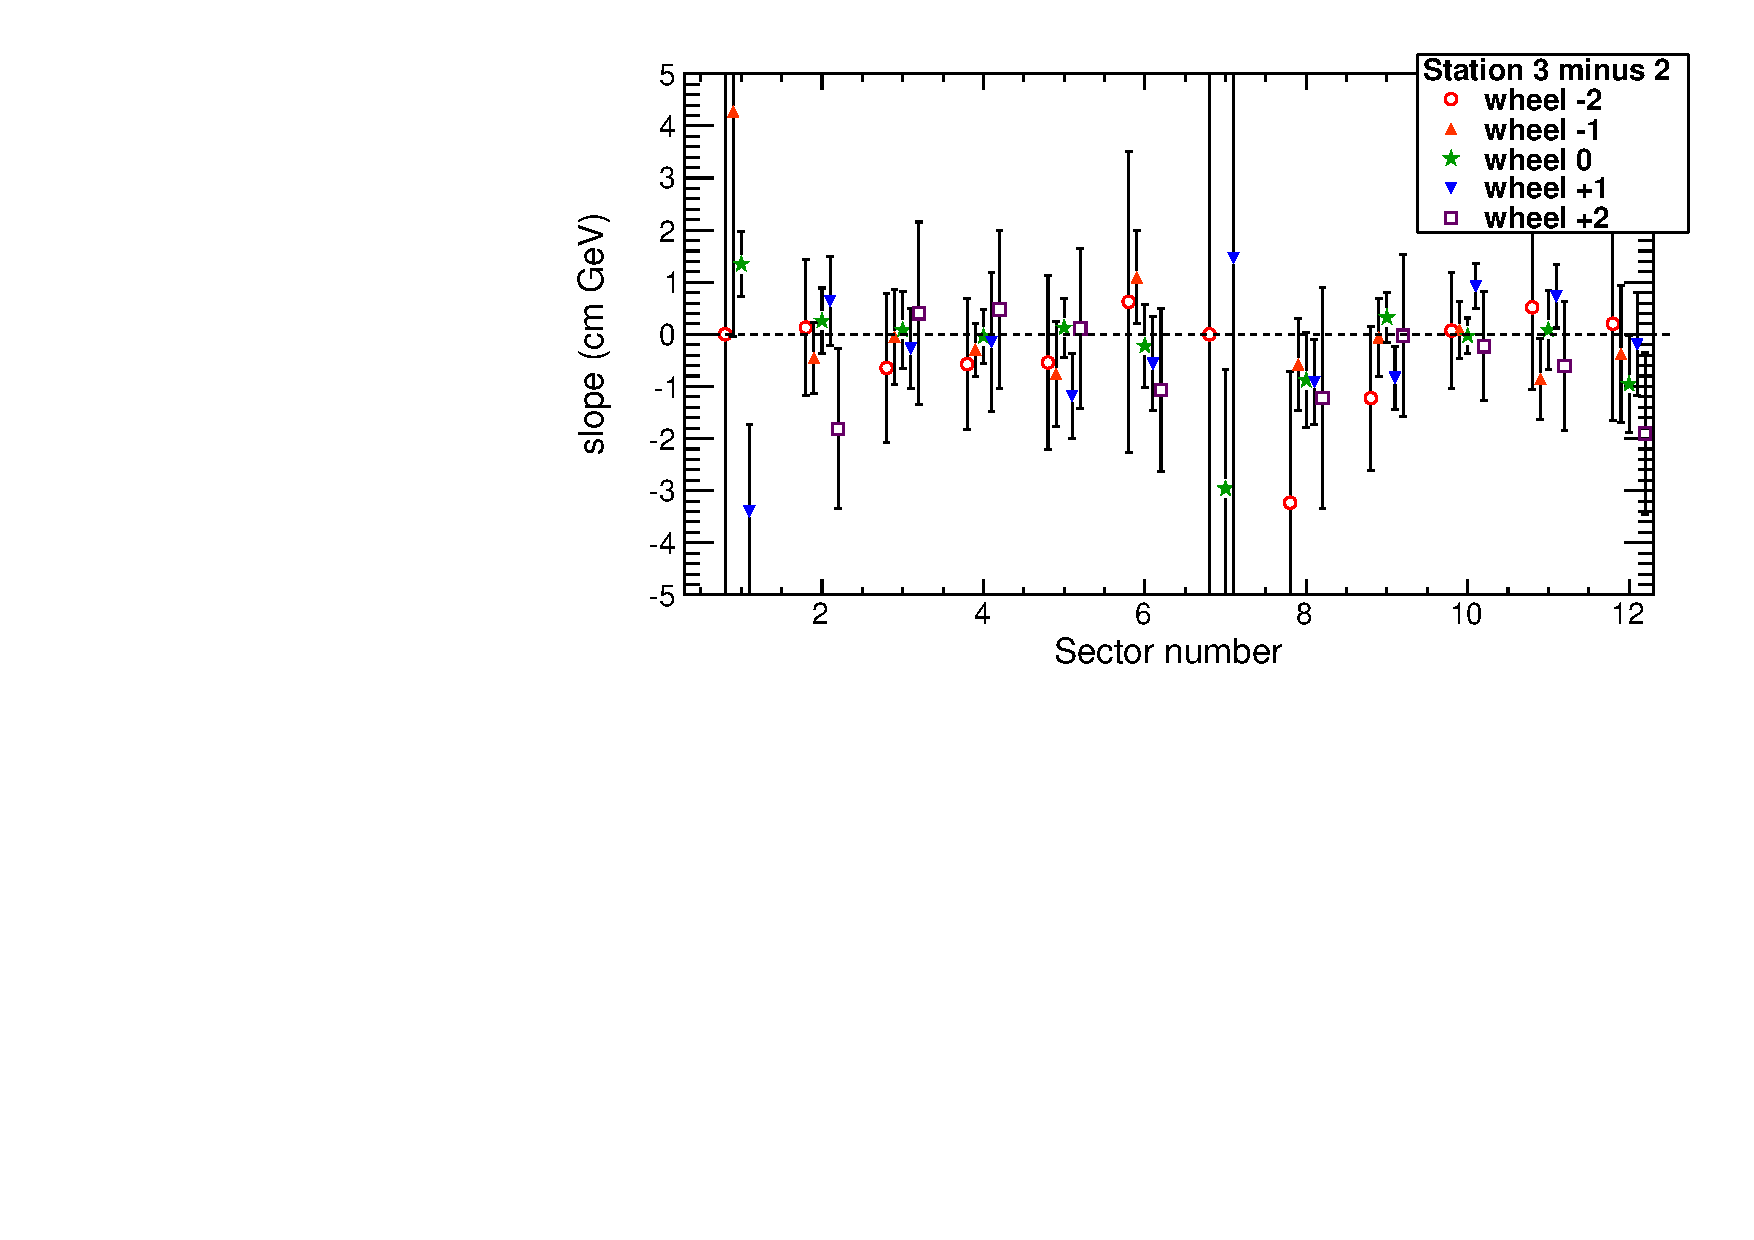
\includegraphics[width=\linewidth]{bfield_slopes_23.pdf}}
\only<3>{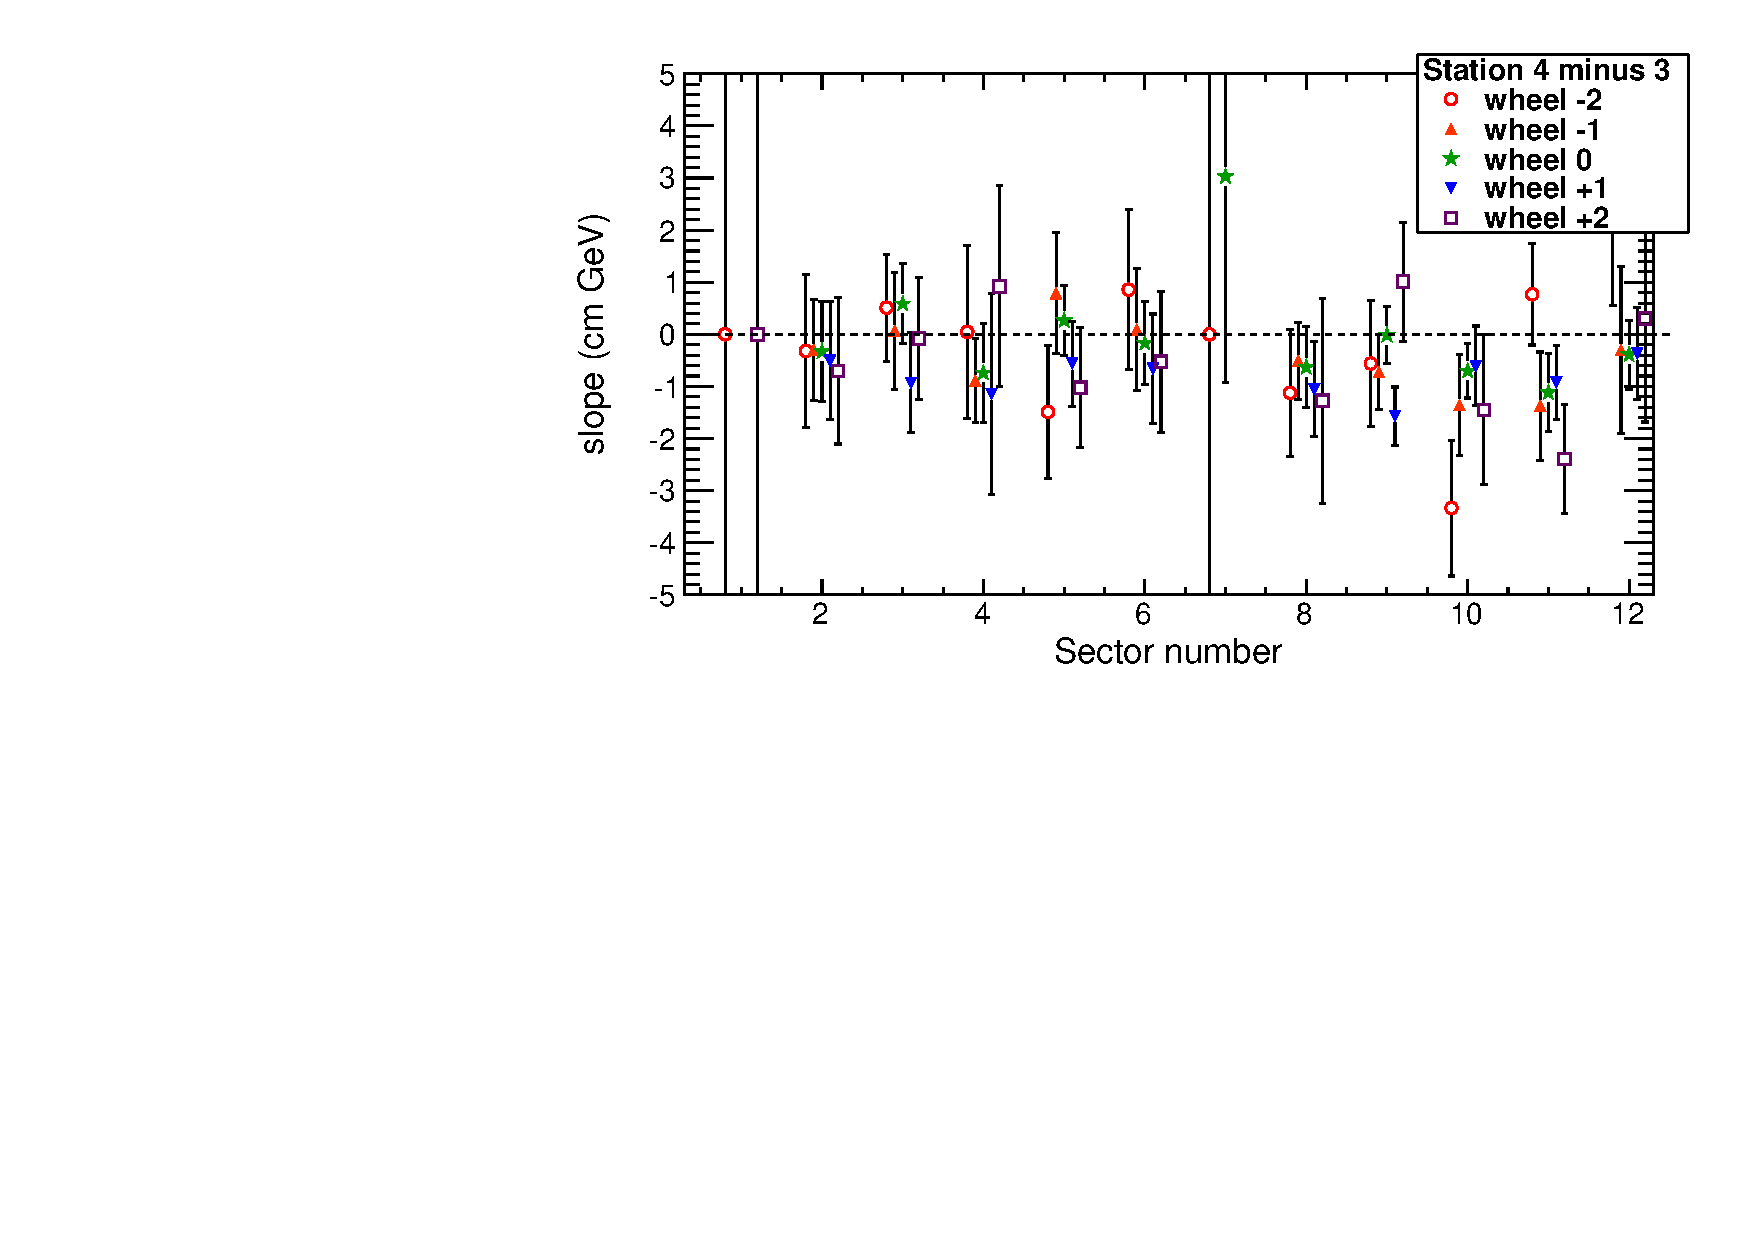
\includegraphics[width=\linewidth]{bfield_slopes_34.pdf}}

\vspace{-1 cm}
\[ \hspace{-0.75 cm} \Delta x \cdot p_T = \frac{\ell^2}{2 (333~\mbox{cm})} 3.8~\mbox{T} \left(\frac{\Delta B}{B}\right) = \left\{\begin{array}{l l} 0.57~\mbox{cm} & \mbox{\scriptsize for $\ell$ = 100~cm} \\ 0.14~\mbox{cm} & \mbox{\scriptsize for $\ell$ = 50~cm} \end{array} \right. \mbox{ and } \frac{\Delta B}{B} = 1\% \]

\vspace{-0.25 cm}
\hfill \textcolor{darkblue}{\scriptsize CRAFT-10}

\vspace{0.25 cm}
\end{frame}

\begin{frame}
\frametitle{Tracker weak mode study}

\begin{columns}
\column{0.5\linewidth}
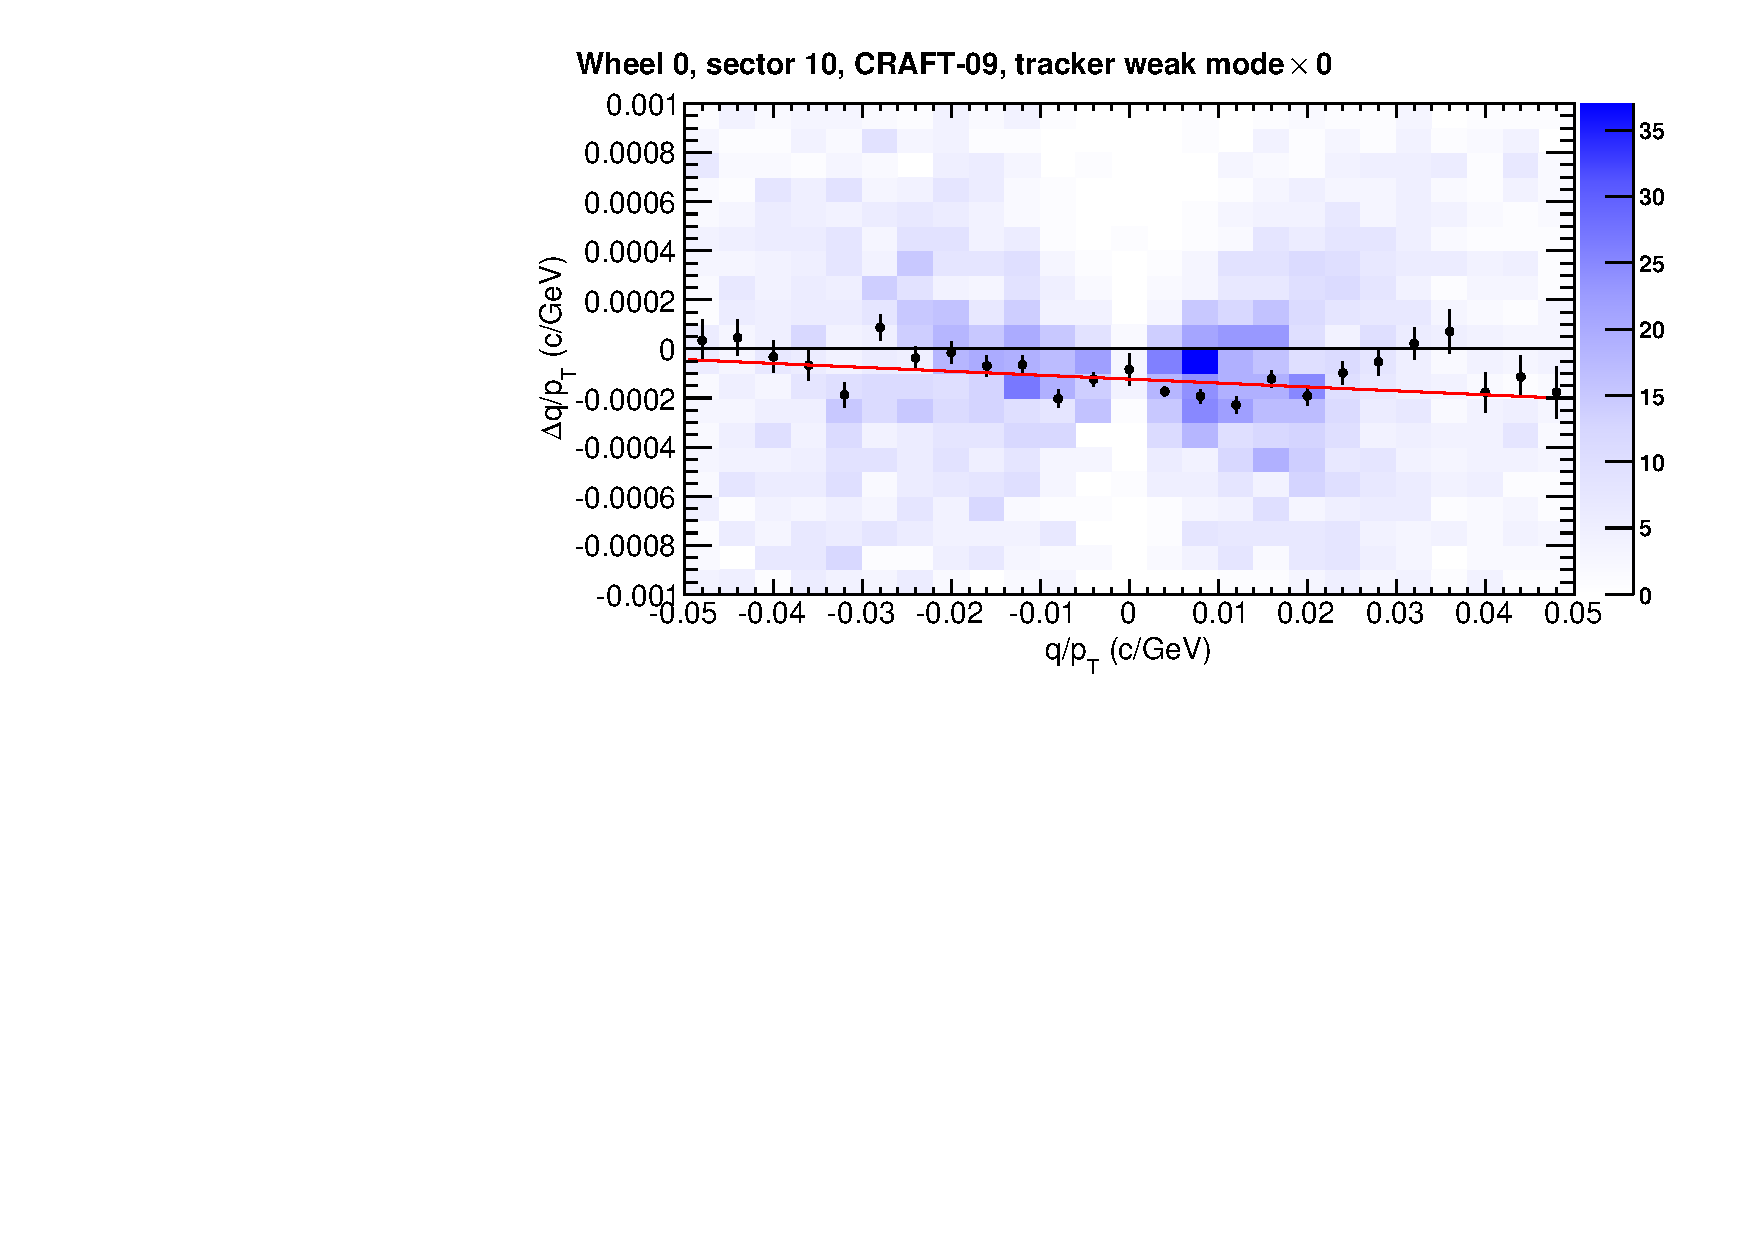
\includegraphics[width=\linewidth]{weakmode_times0.pdf}

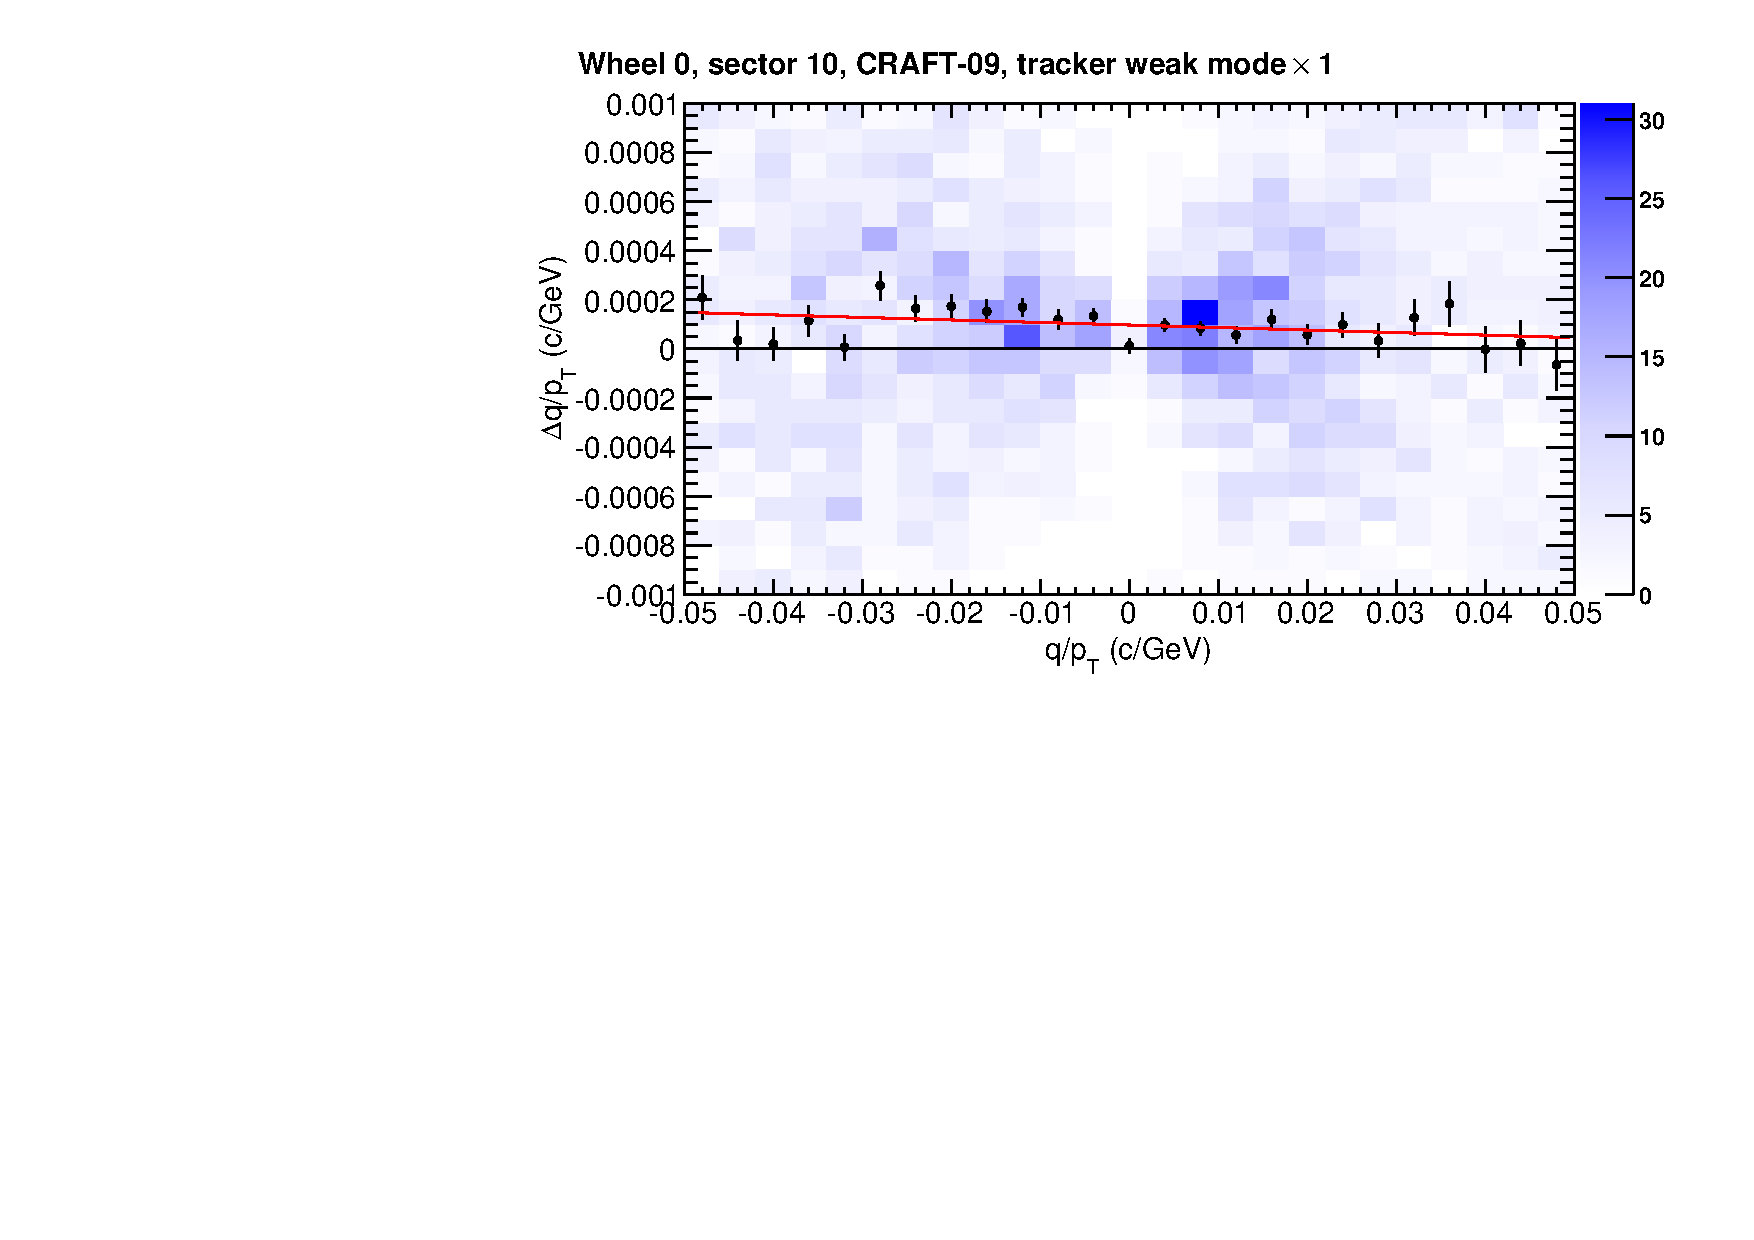
\includegraphics[width=\linewidth]{weakmode_times1.pdf}

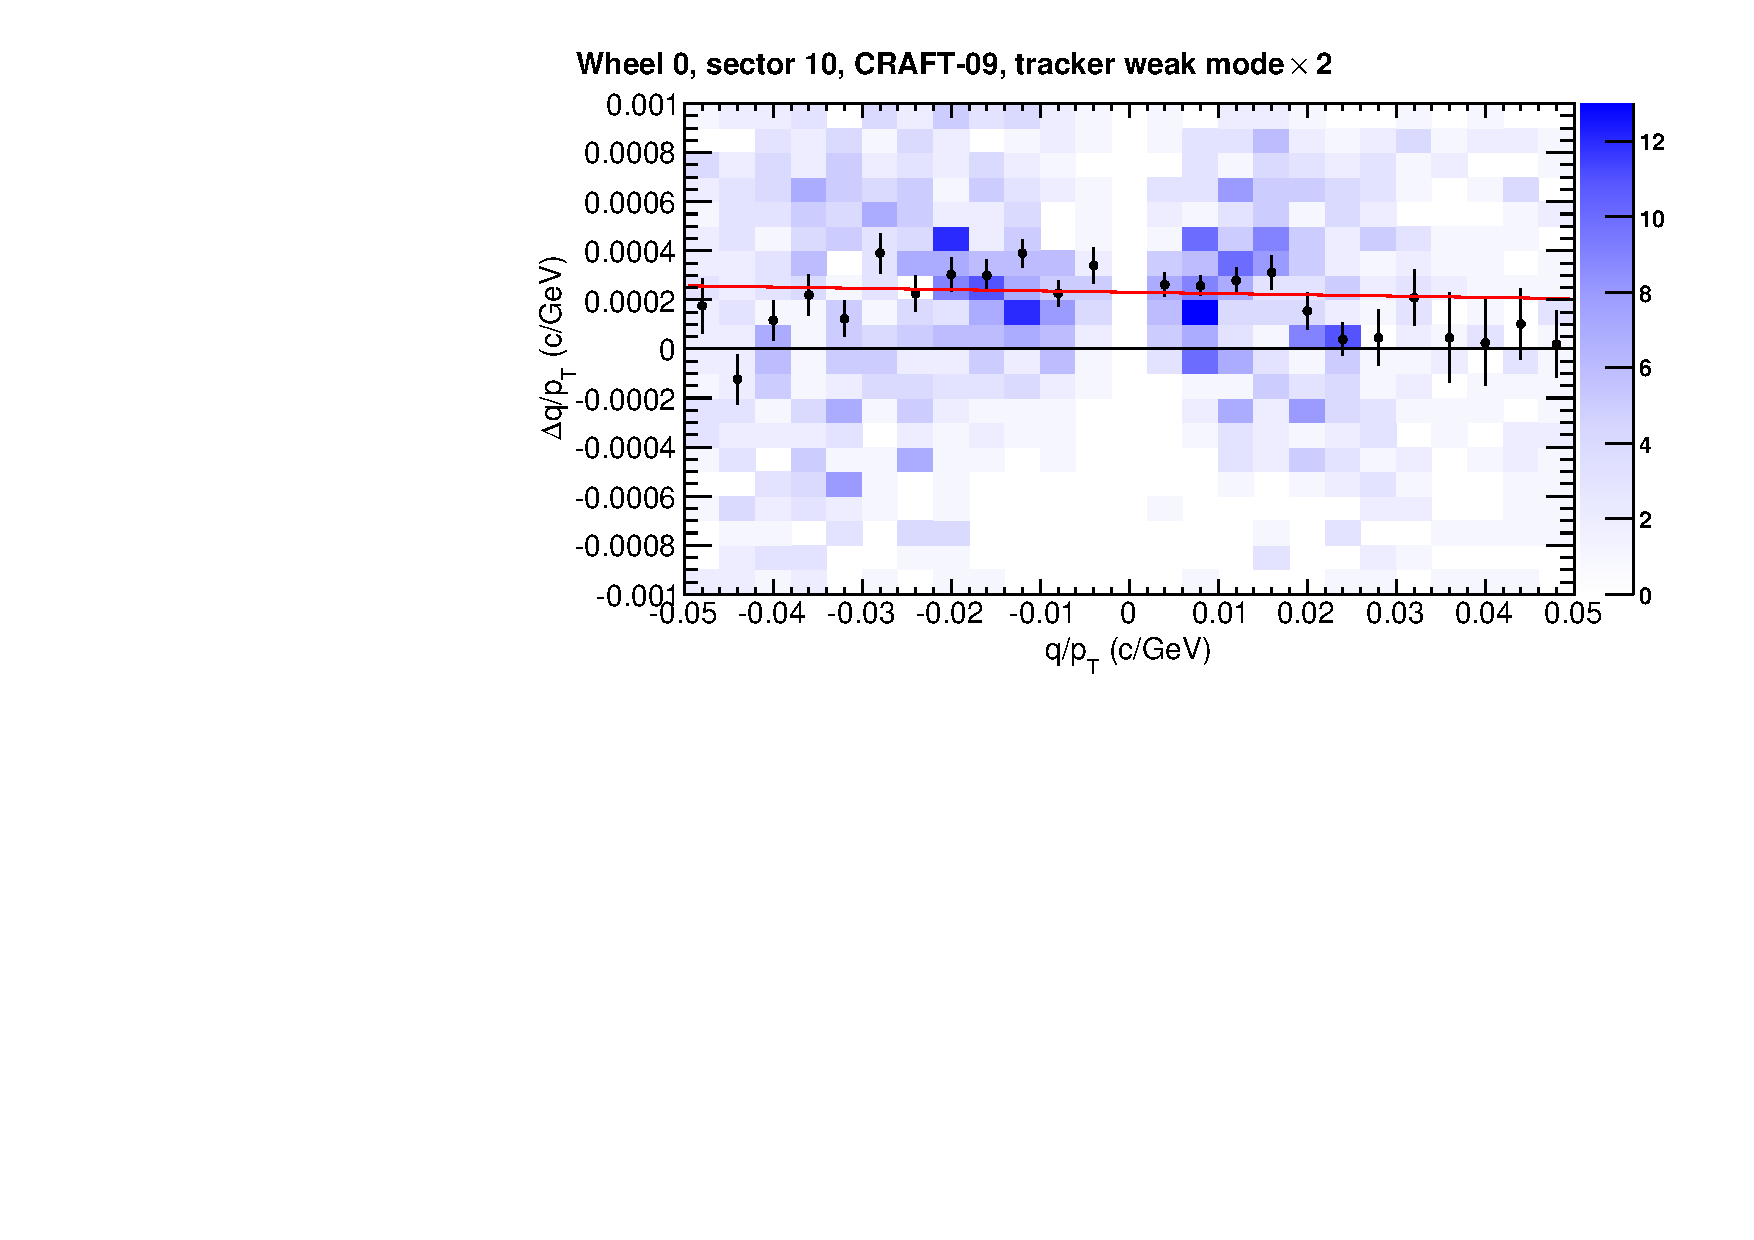
\includegraphics[width=\linewidth]{weakmode_times2.pdf}

\column{0.5\linewidth}

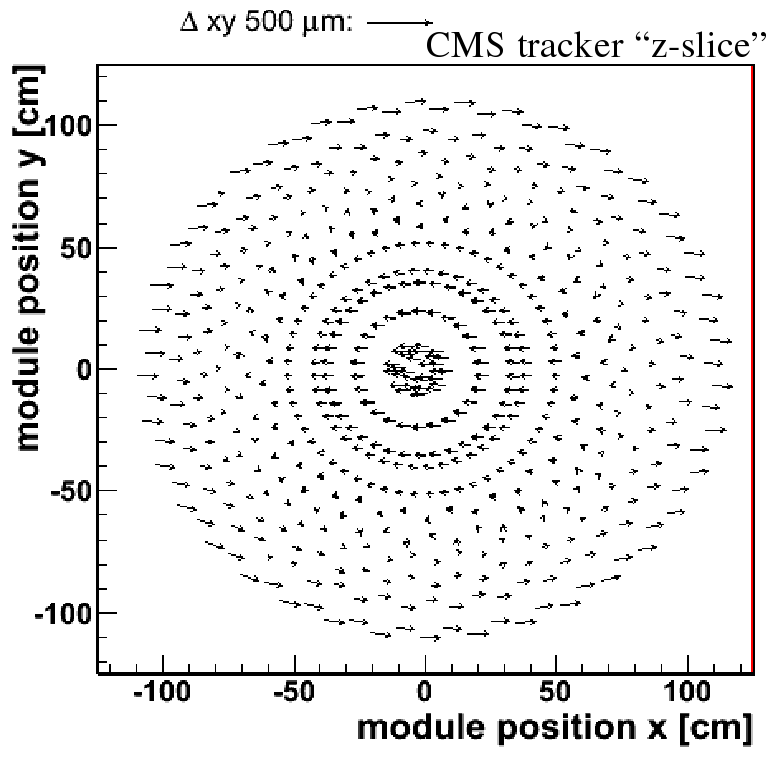
\includegraphics[width=0.5\linewidth]{stoye_deformation.png}
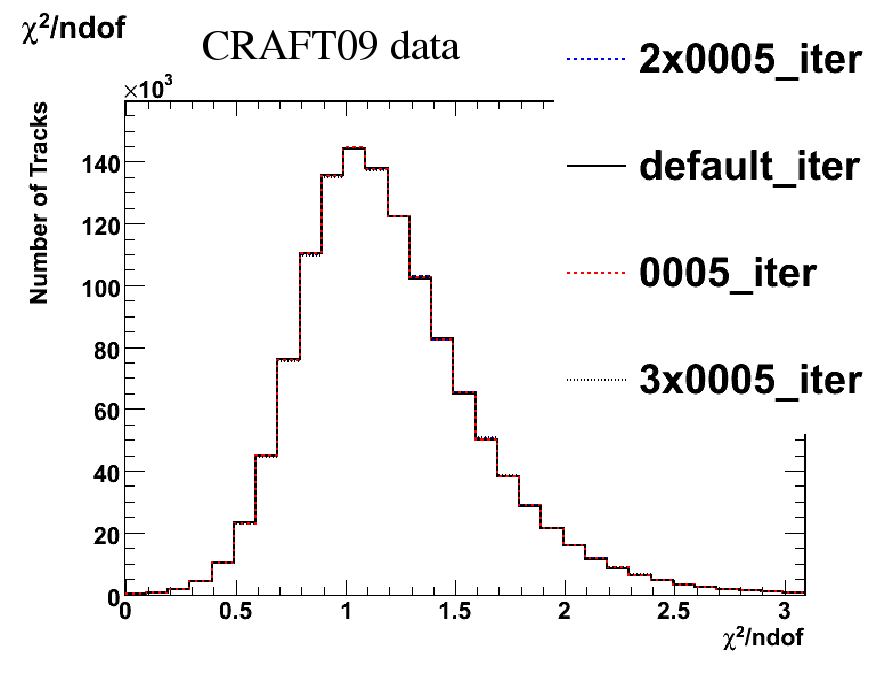
\includegraphics[width=0.5\linewidth]{chi2_invariance.png}

\begin{itemize}
\item Apply Millepede-generated mode to correctly-calculated muon residuals

\item No distortion with ``100~GeV/$c$ characteristic scale'': that was the RPCs

\item Only a constant shift in $\Delta(q/p_T)$
\end{itemize}

\hfill \textcolor{darkblue}{\scriptsize CRAFT-09}
\end{columns}
\end{frame}

\begin{frame}
\frametitle{Tracker weak mode study}

\begin{itemize}
\item How are the ``constant shifts in $\Delta(q/p_T)$'' distributed?  (i.e.\ $\Delta x$?)
\end{itemize}

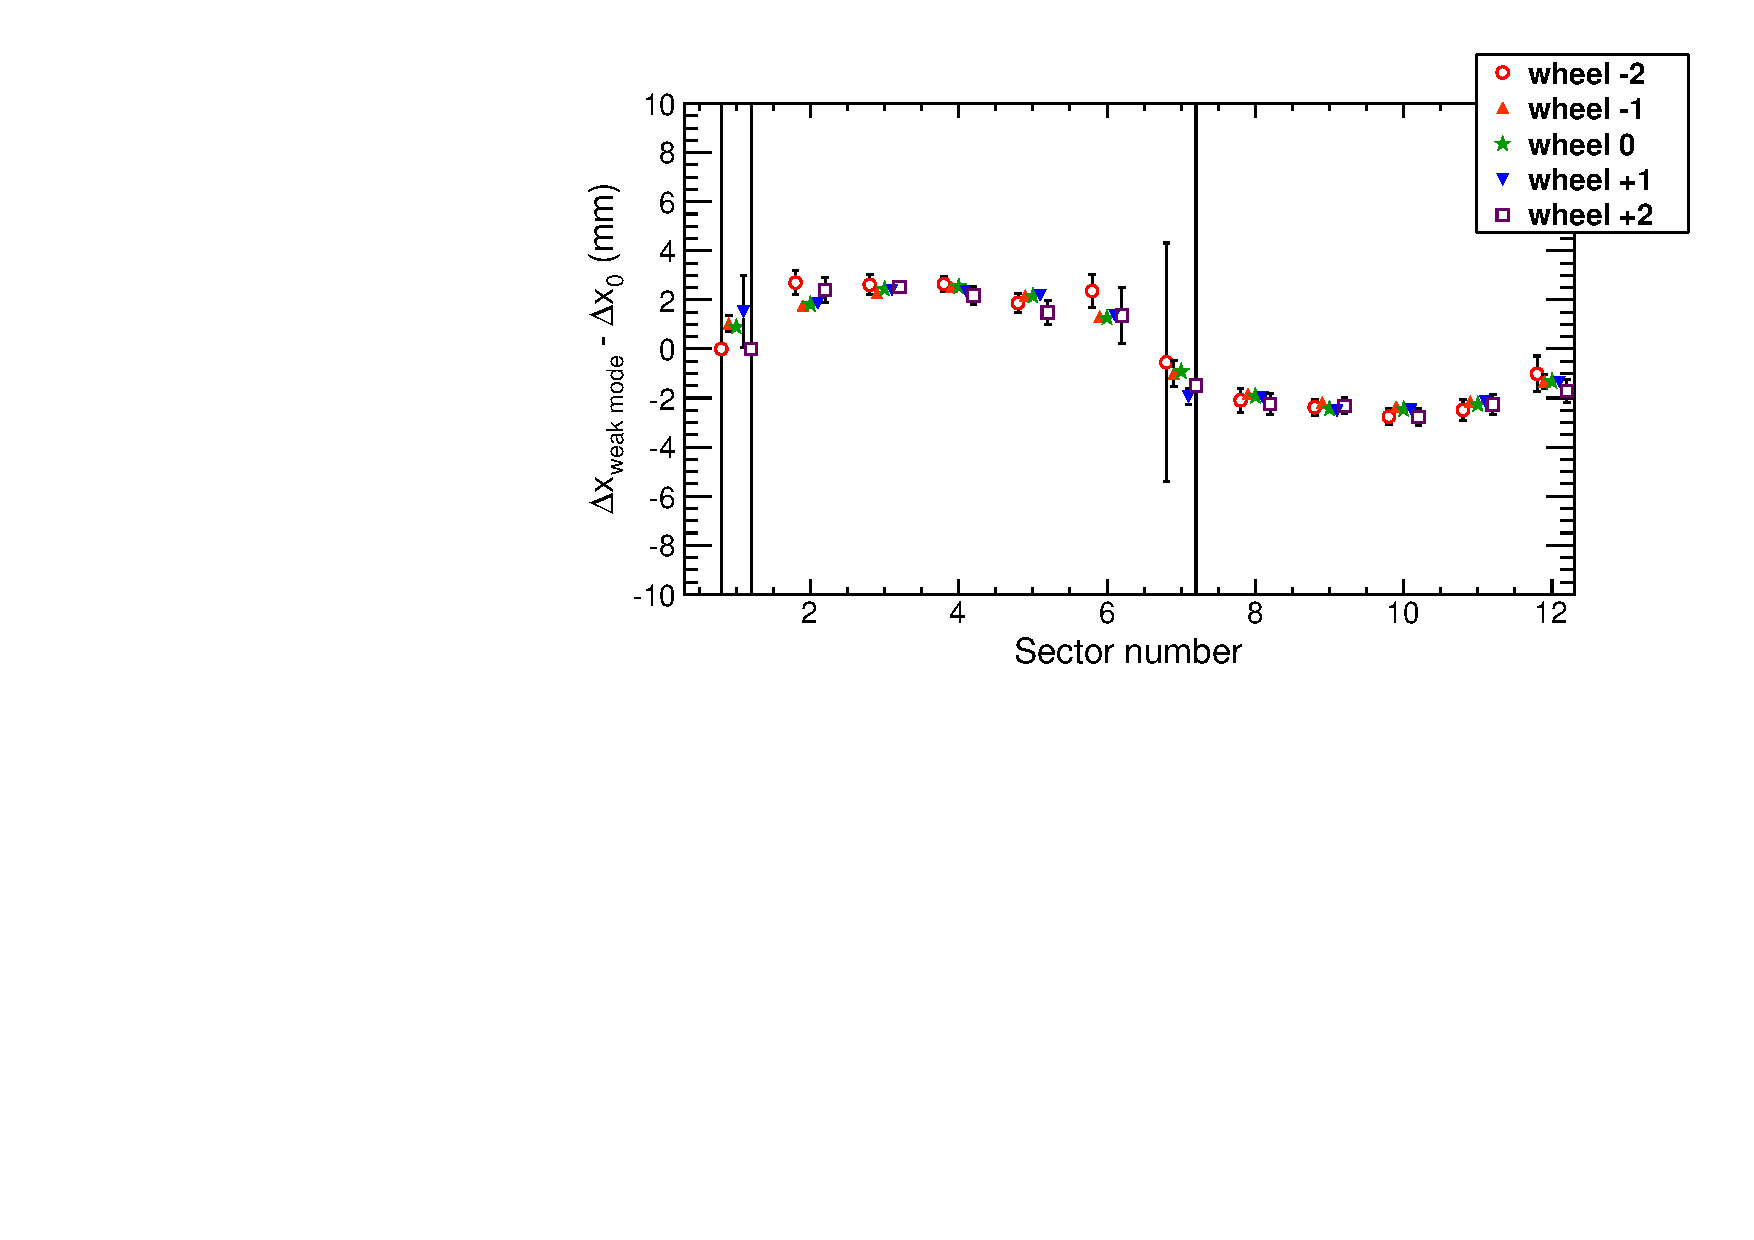
\includegraphics[width=\linewidth]{weakmode_xsummary1.pdf}

\begin{itemize}
\item Sinusoidally, which implies nothing more than a global $x$
  translation between the ``weak mode'' tracker geometry and the
  normal tracker
\end{itemize}

\hfill \textcolor{darkblue}{\scriptsize CRAFT-09}
\end{frame}

\begin{frame}
\frametitle{Tracker weak mode study}
\begin{itemize}\setlength{\itemsep}{0.25 cm}
\item Conclusion: muon residuals are {\it insensitive} to the
  Millepede-generated weak mode

\item Implication: we cannot use muon residuals to bound this kind of
  distortion in the tracker (constant $\Delta(q/p_T)$)

\item Bound from Cosmics Endpoint is still valid: $\sim$0.05~$c$/TeV

\item In muon station~1, $\Delta x$ = 1~mm is $\Delta(q/p_T)$ = 0.2~$c$/TeV

so error in muon alignment from tracker $\Delta(q/p_T)$ bias is $\sim$0.25~mm in station~1

\item Independent of $p_T$; we can now loosen the cut for higher
  statistics (and alignments using collisions muons)
\begin{itemize}
\item keep in mind that resolution vs.\ integrated luminosity will need to be revised (residuals distributions are wider)
\end{itemize}
\end{itemize}
\end{frame}

\begin{frame}
\frametitle{New 2010 muon alignment}

\begin{enumerate}
\item Re-ran 2010 muon alignment without RPC bias
\item Compare alignment parameters with and without RPC bias
\end{enumerate}

\begin{columns}
\column{0.7\linewidth}
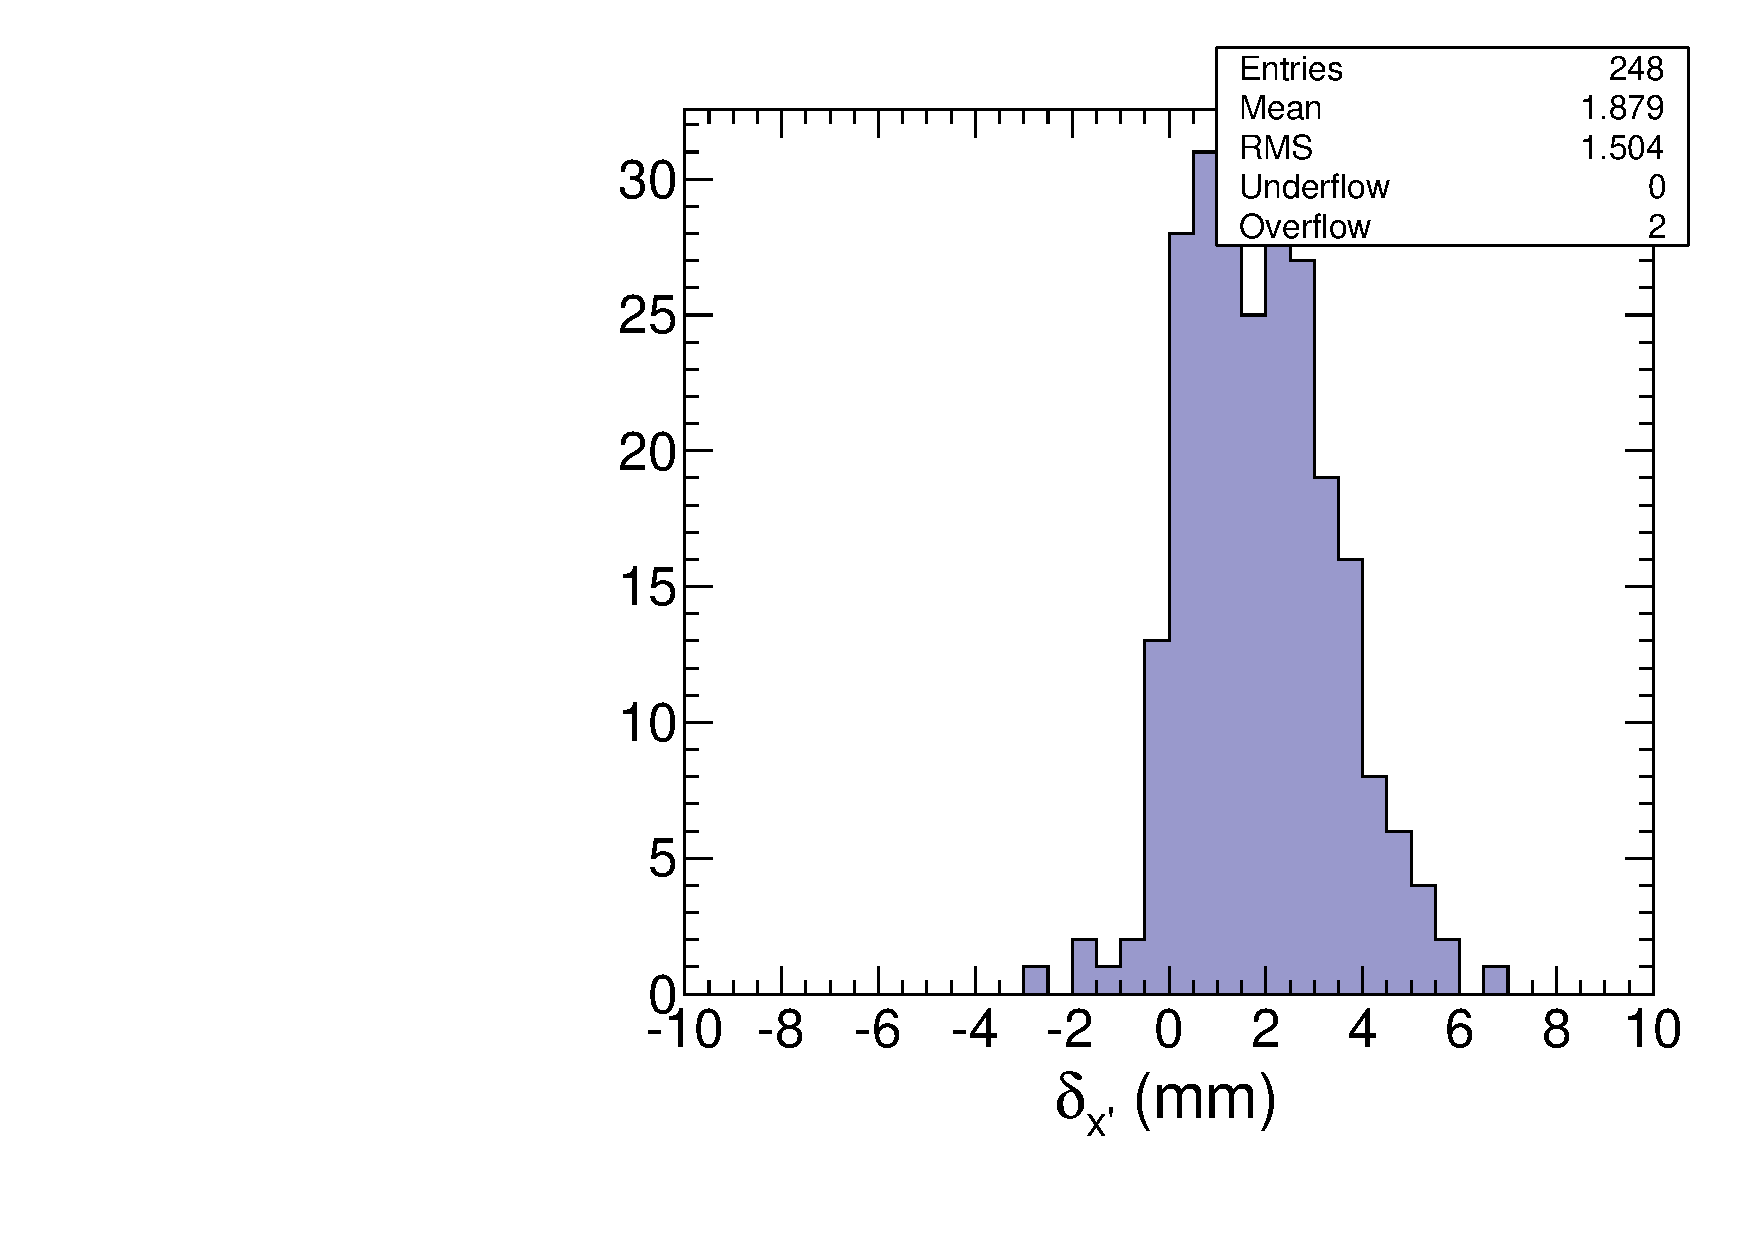
\includegraphics[width=0.5\linewidth]{01_deltax_with_and_without_RPC.pdf}
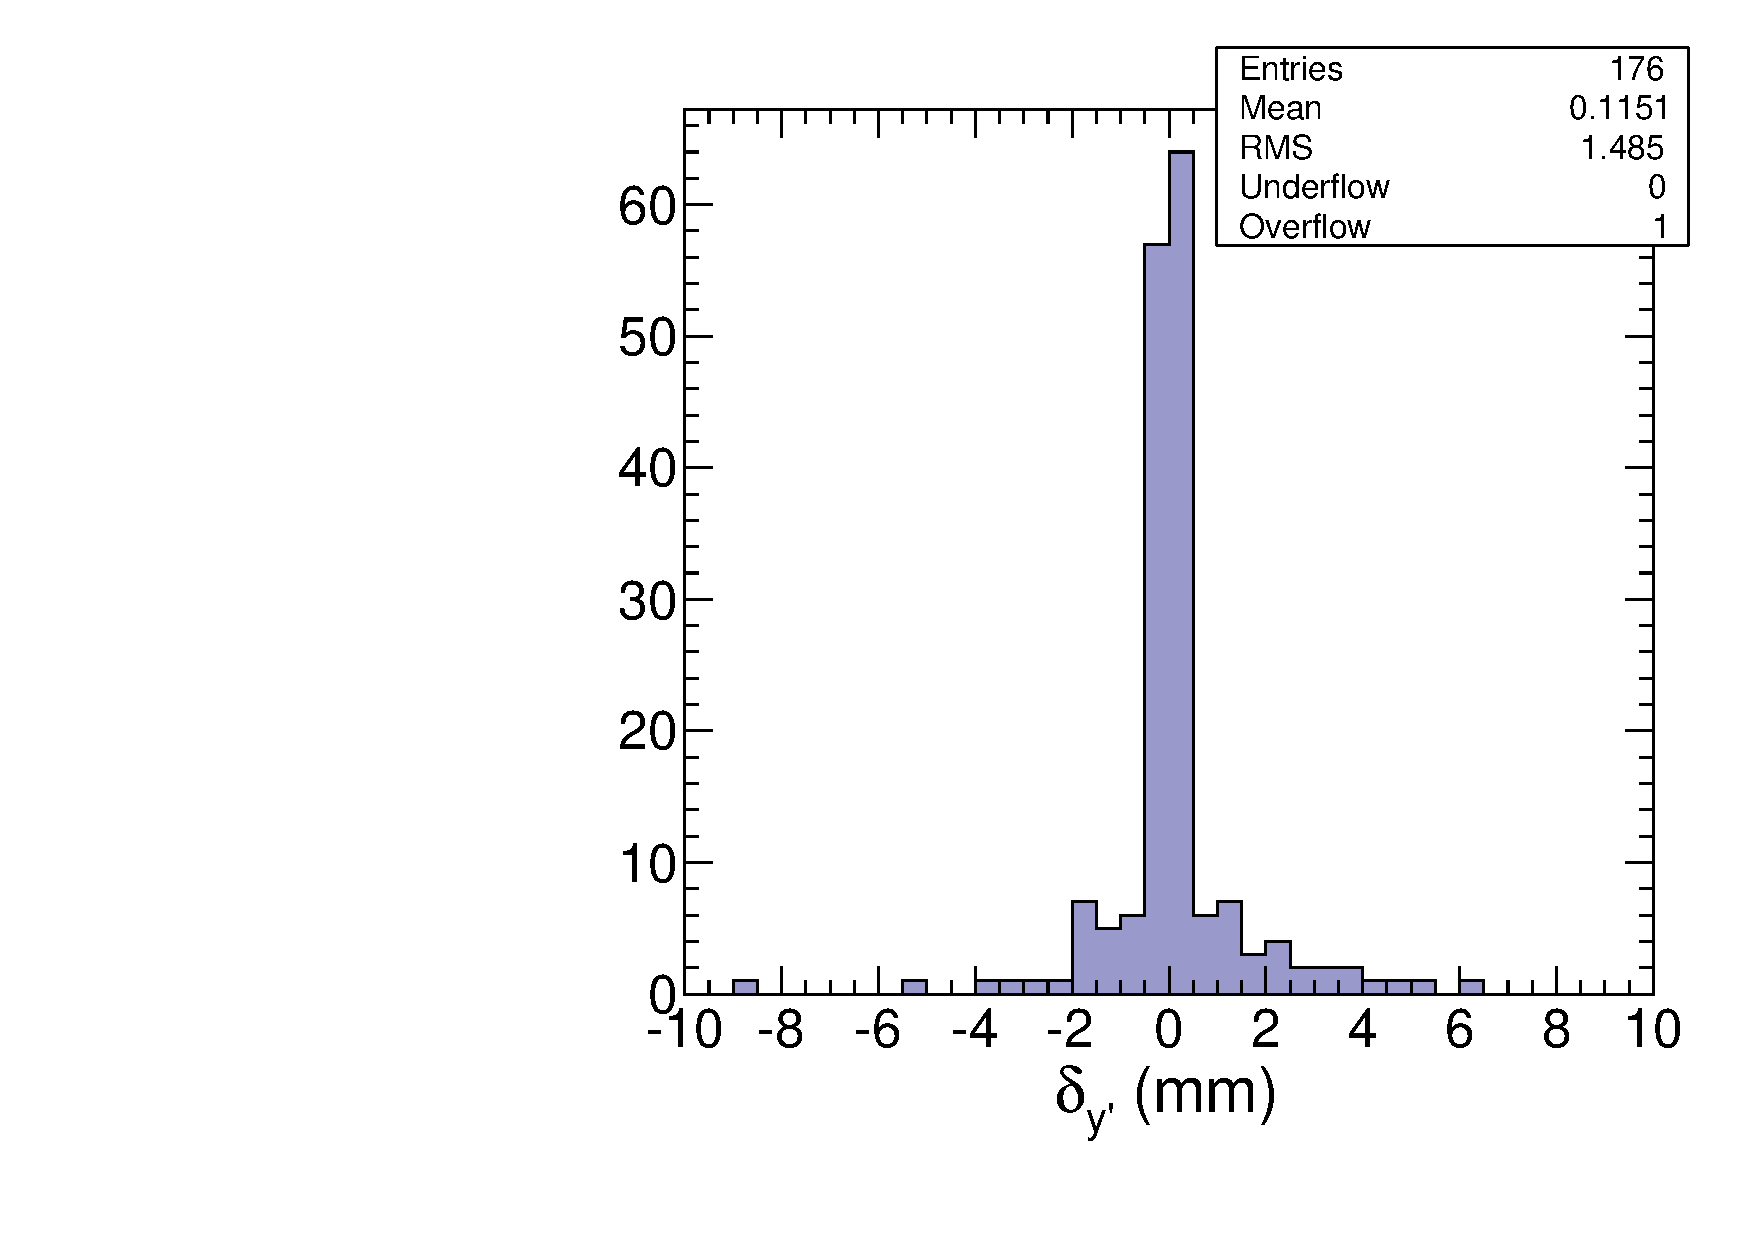
\includegraphics[width=0.5\linewidth]{02_deltay_with_and_without_RPC.pdf}

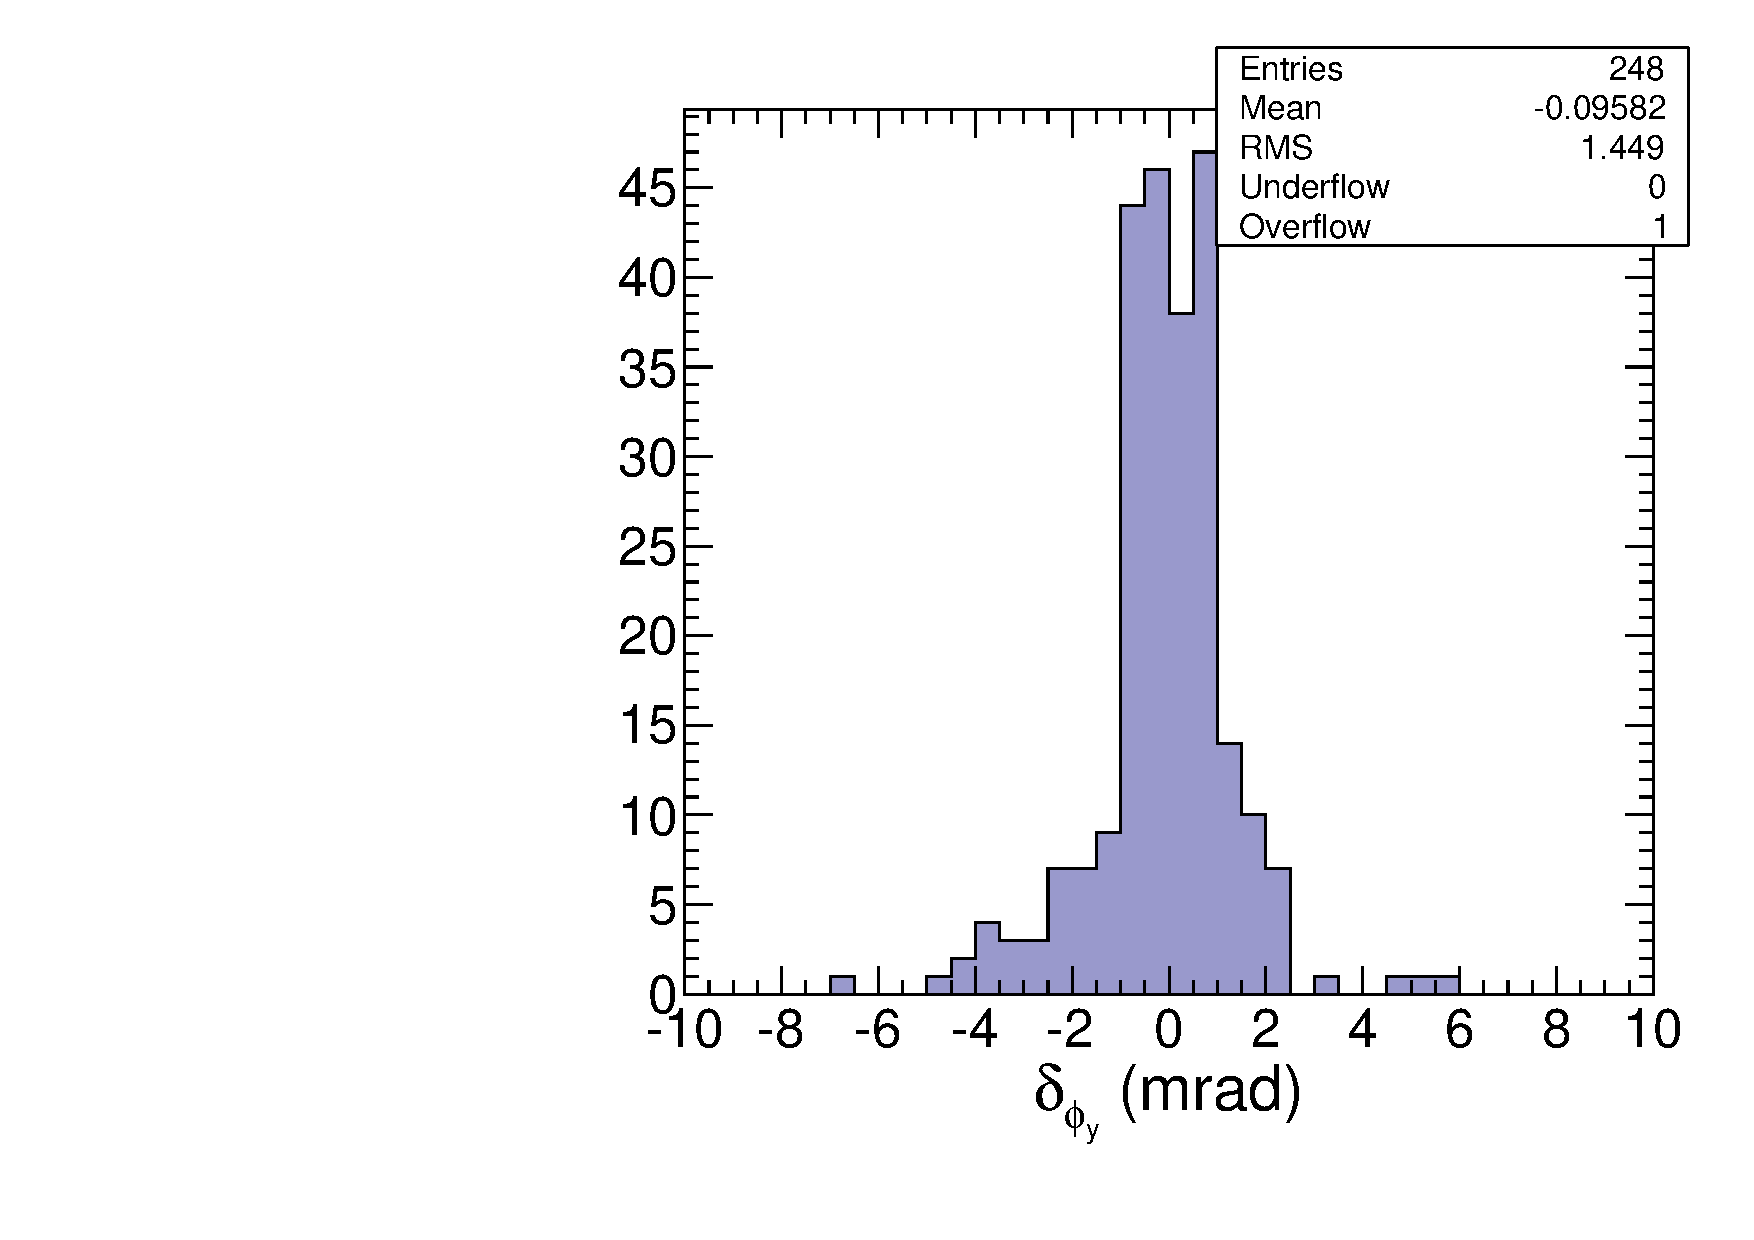
\includegraphics[width=0.5\linewidth]{03_deltaphiy_with_and_without_RPC.pdf}
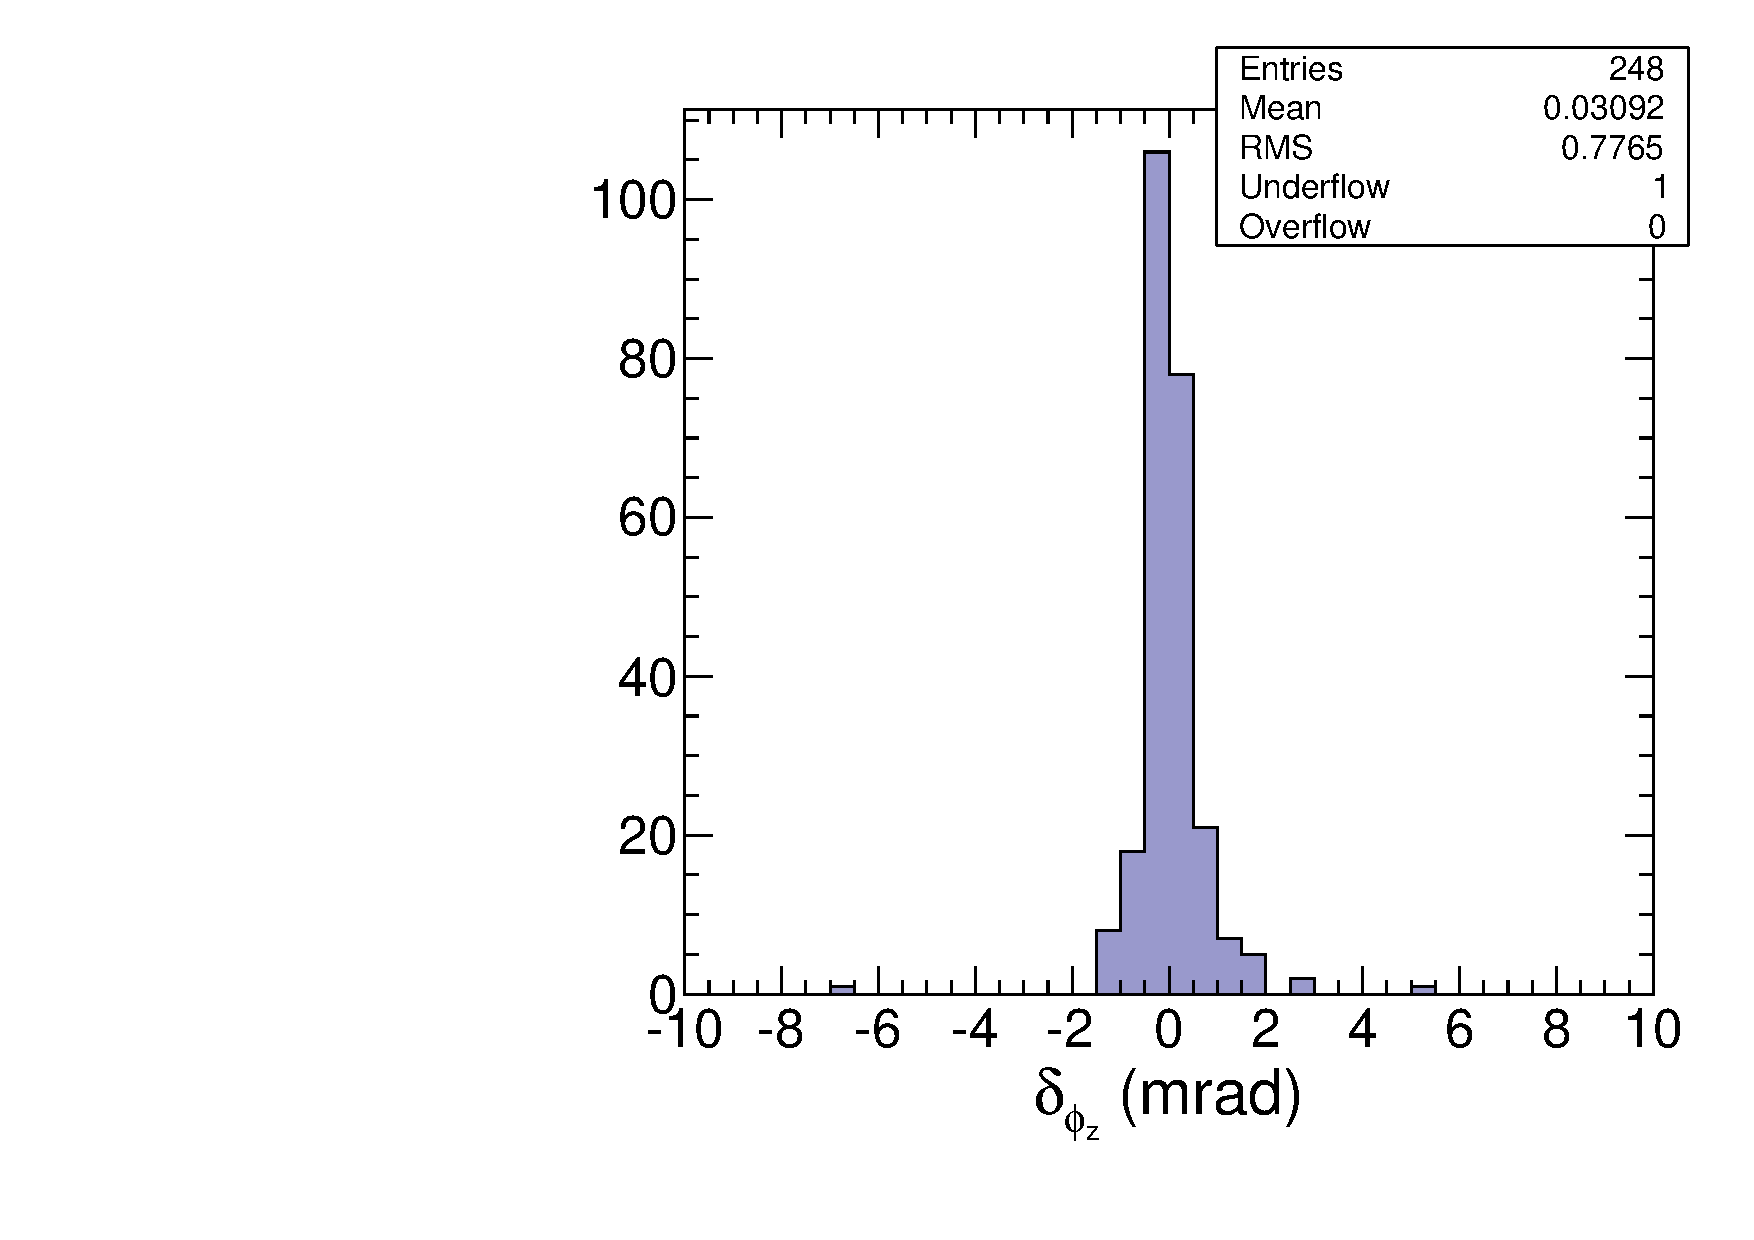
\includegraphics[width=0.5\linewidth]{04_deltaphiz_with_and_without_RPC.pdf}

\column{0.3\linewidth}
\begin{itemize}
\item Effective rotation of about 0.3~mrad
\item RMS spread of 1.5~mm
\item Most chamber $y$ are unaffected
\item Double-peak in $\phi_y$ is related to rotation and local sign conventions
\end{itemize}

\hfill \textcolor{darkblue}{\scriptsize CRAFT-10}
\end{columns}
\end{frame}

\begin{frame}
\frametitle{New 2010 muon alignment}

(Comparing alignment with RPC bias against unbiased alignment)

\begin{itemize}
\item Structure vs.\ $\phi$ not exactly sinusoidal; must be related to placement of RPCs somehow
\item No structure vs.\ wheel (RPC bias not responsible for ``barrel twist'')
\end{itemize}

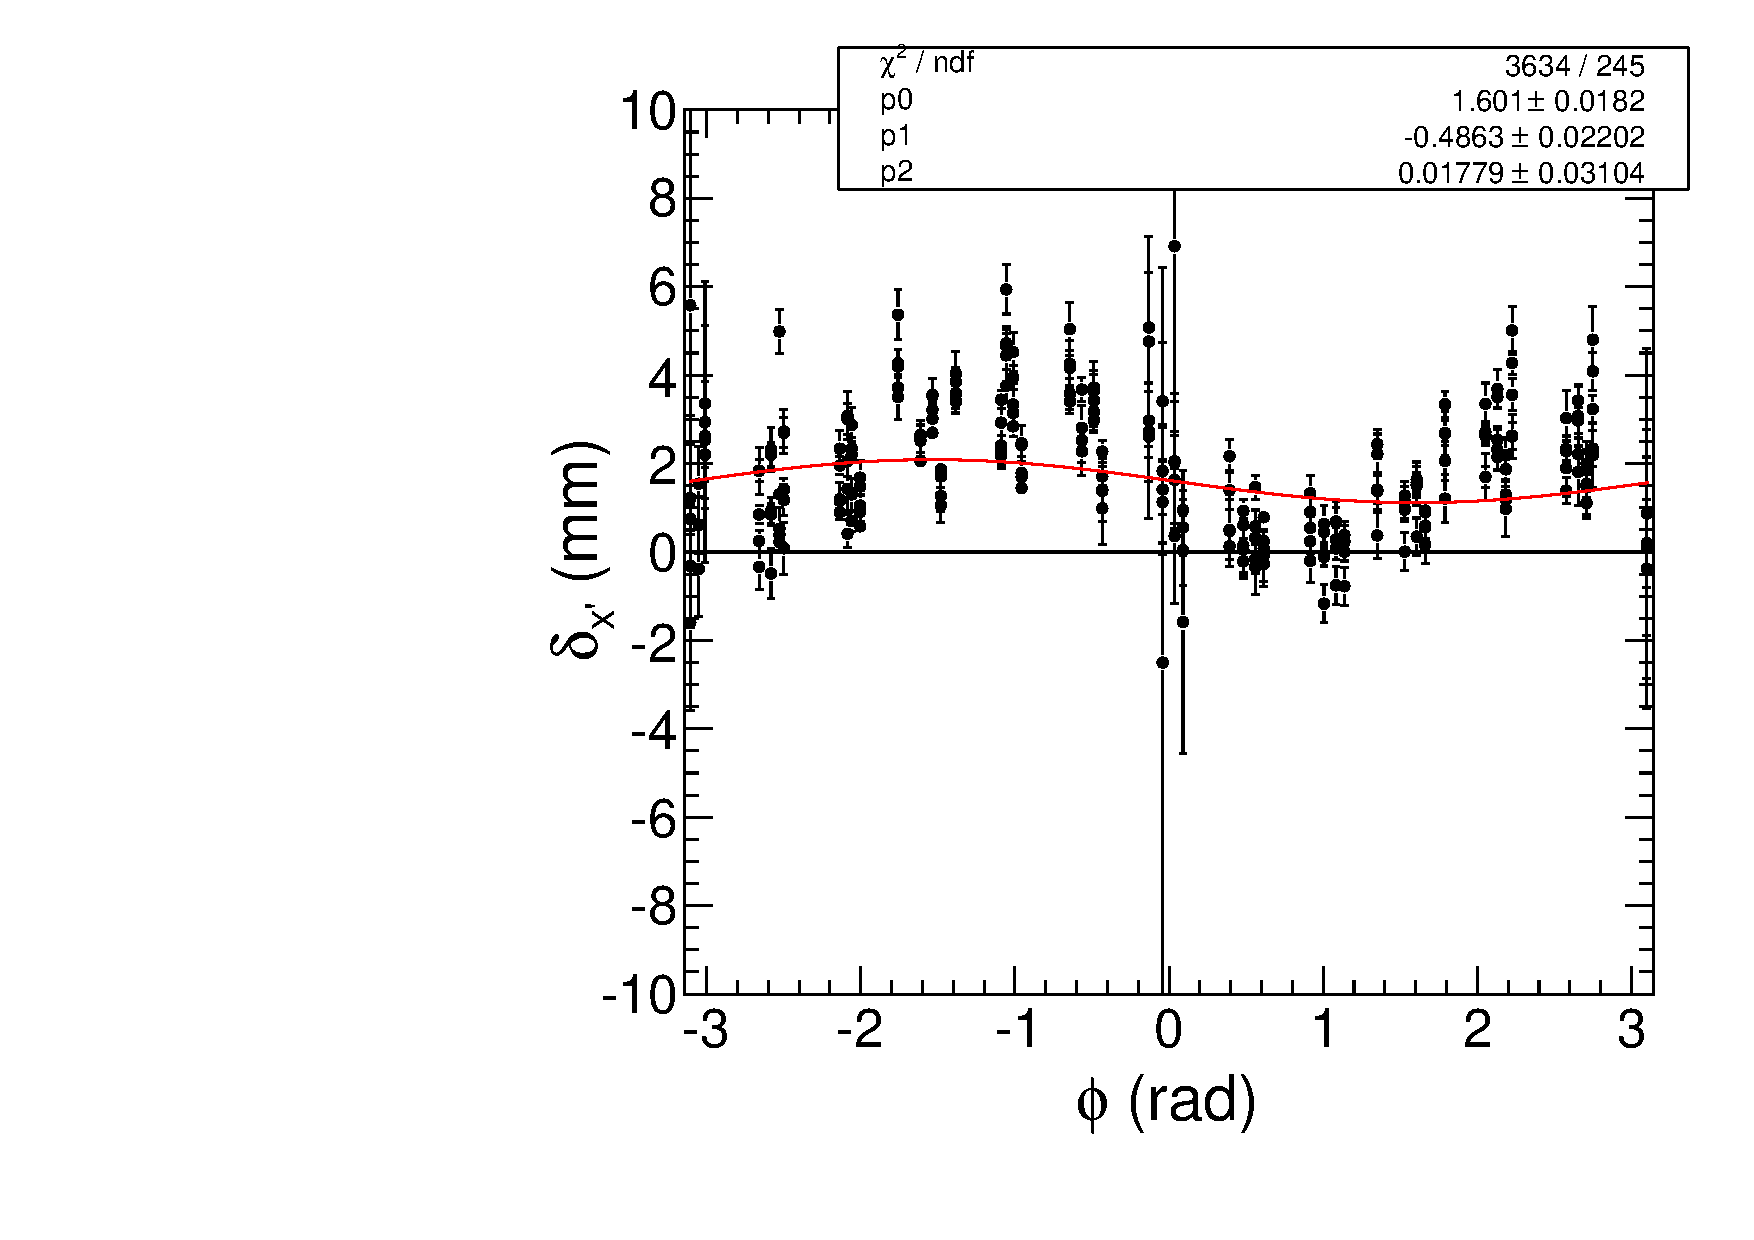
\includegraphics[width=0.5\linewidth]{05_deltax_phi_with_and_without_RPC.pdf}
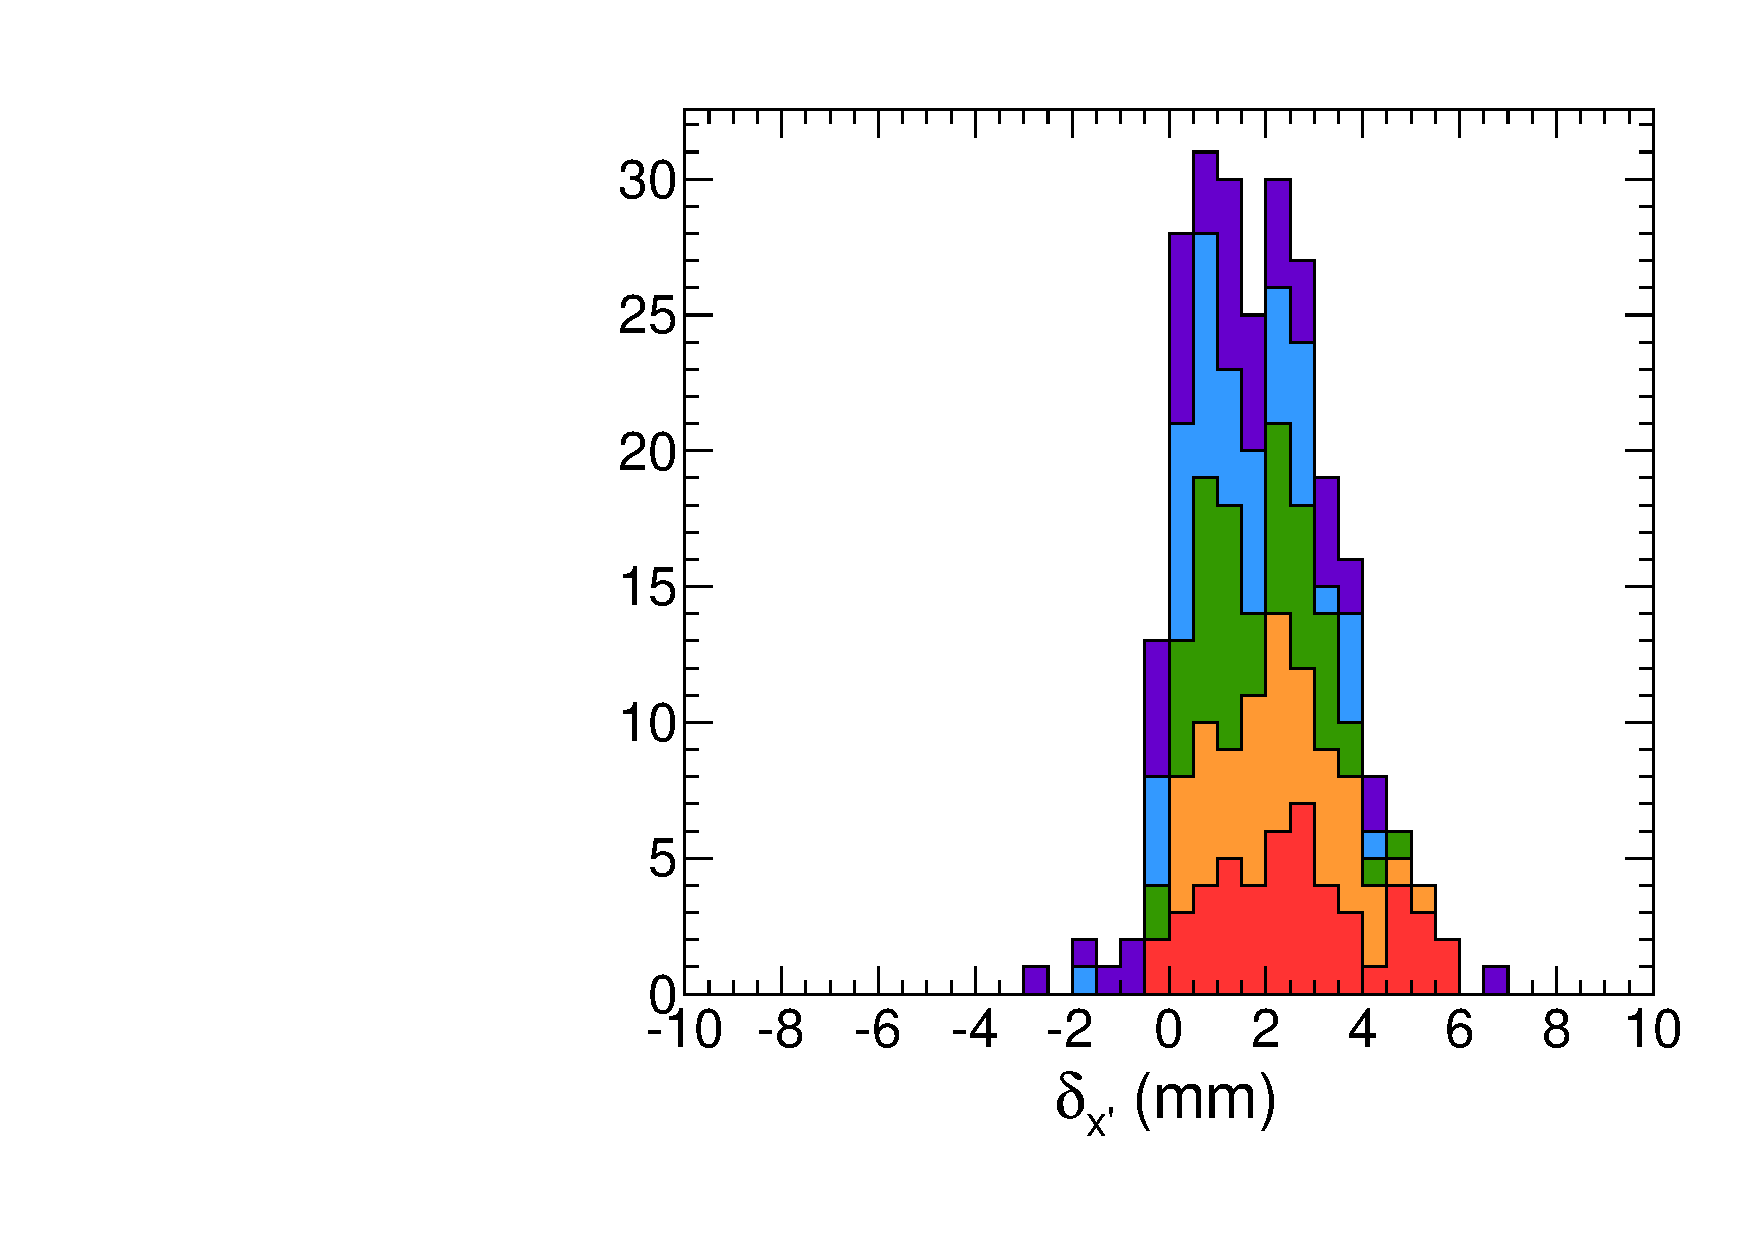
\includegraphics[width=0.5\linewidth]{06_deltax_stack_with_and_without_RPC.pdf}

\hfill \textcolor{darkblue}{\scriptsize CRAFT-10}
\end{frame}

\begin{frame}
\frametitle{New 2010 muon alignment}

\begin{itemize}
\item Now comparing alignment parameters without RPC bias to hardware
\end{itemize}

\begin{columns}
\column{0.7\linewidth}
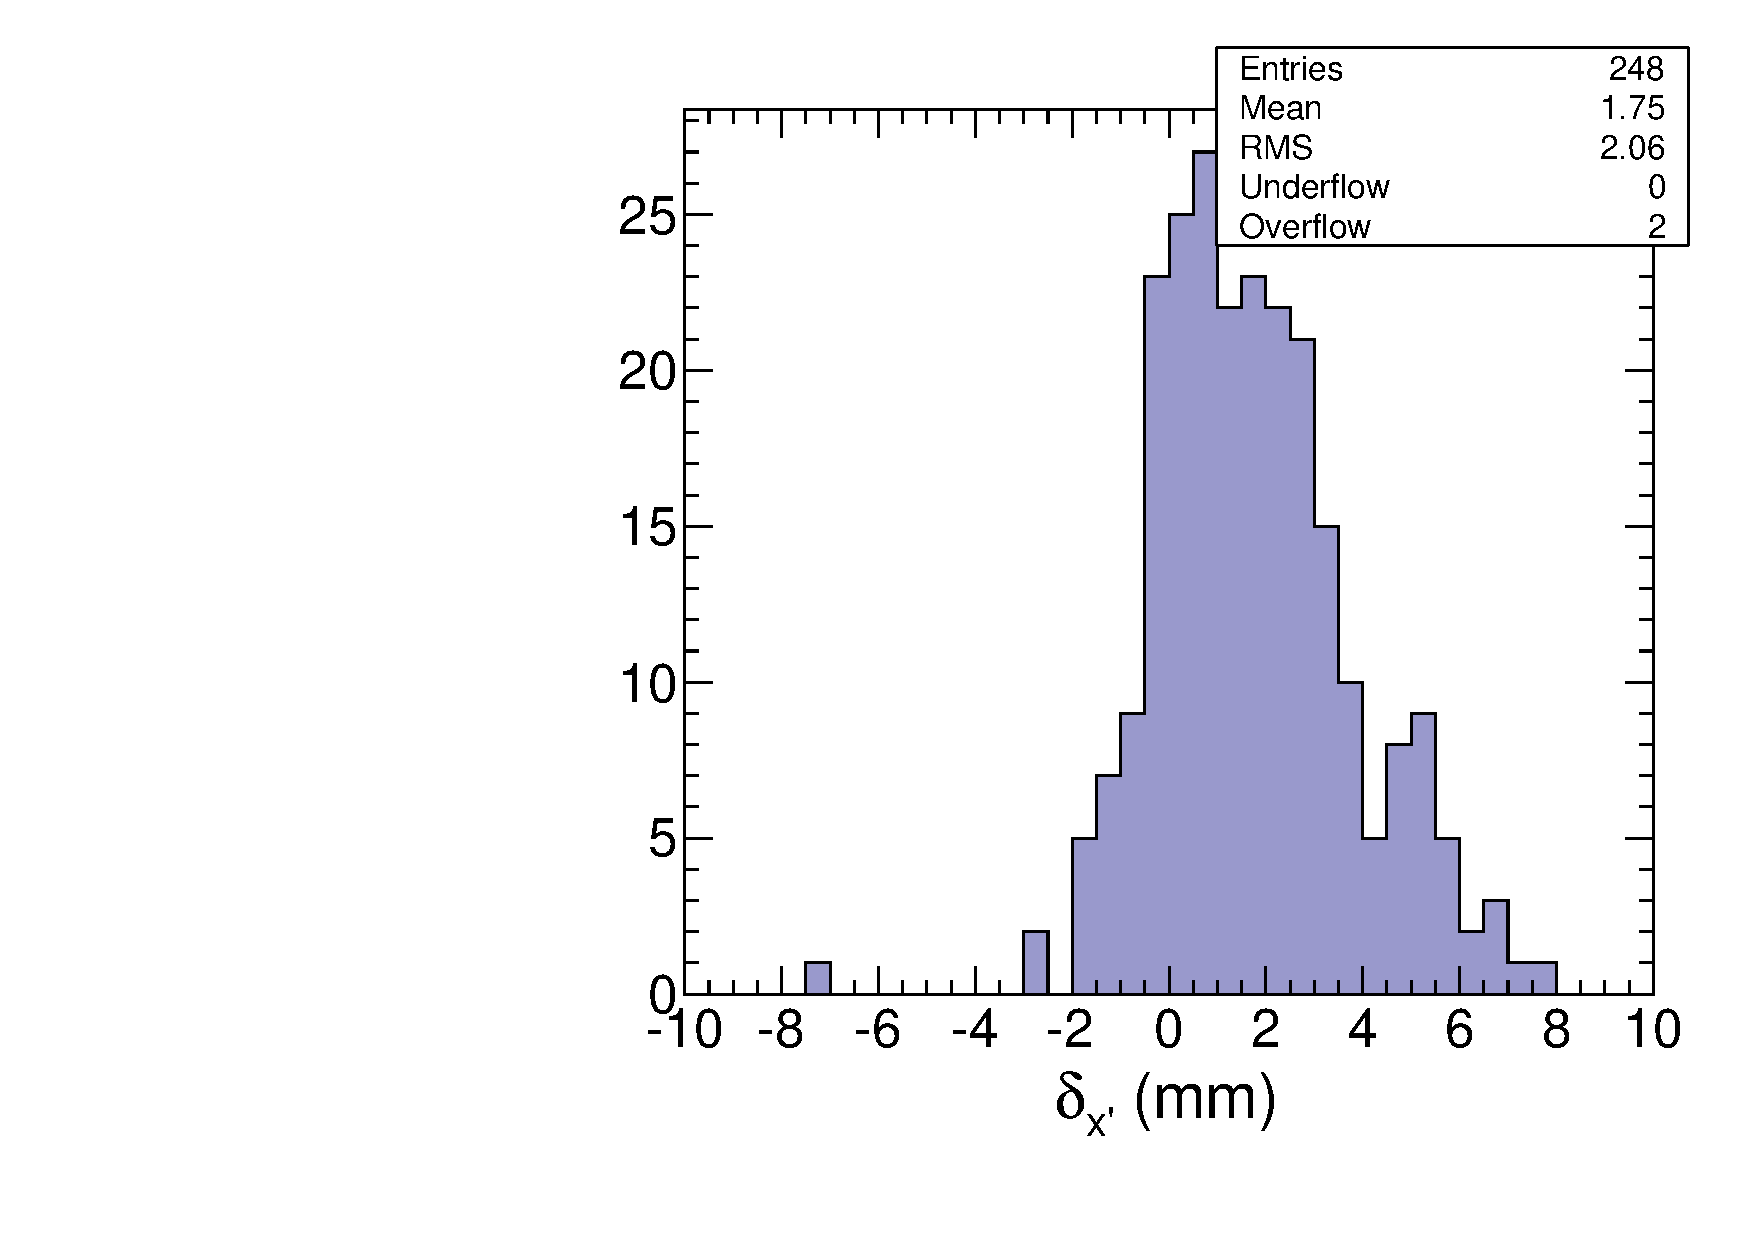
\includegraphics[width=0.5\linewidth]{08_deltax_without_RPC_and_hardware.pdf}
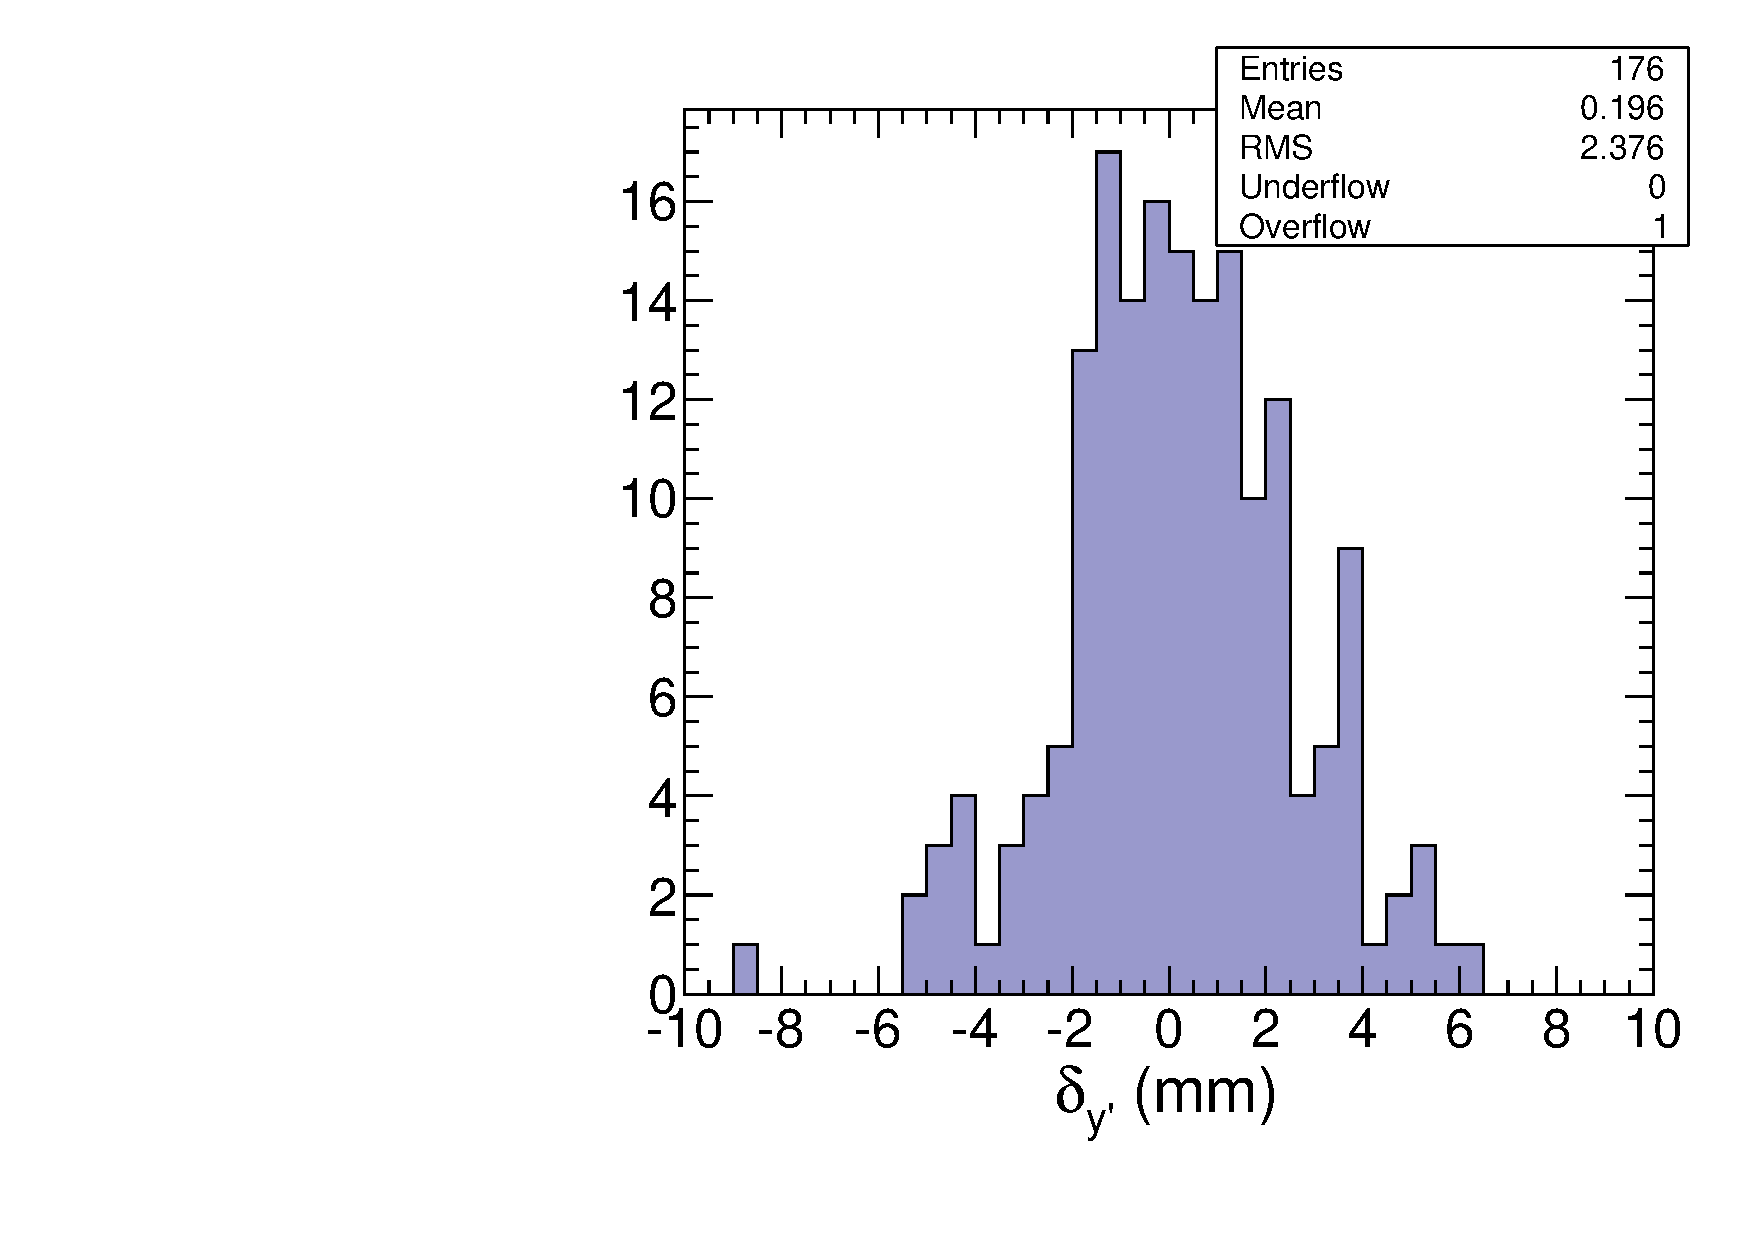
\includegraphics[width=0.5\linewidth]{09_deltay_without_RPC_and_hardware.pdf}

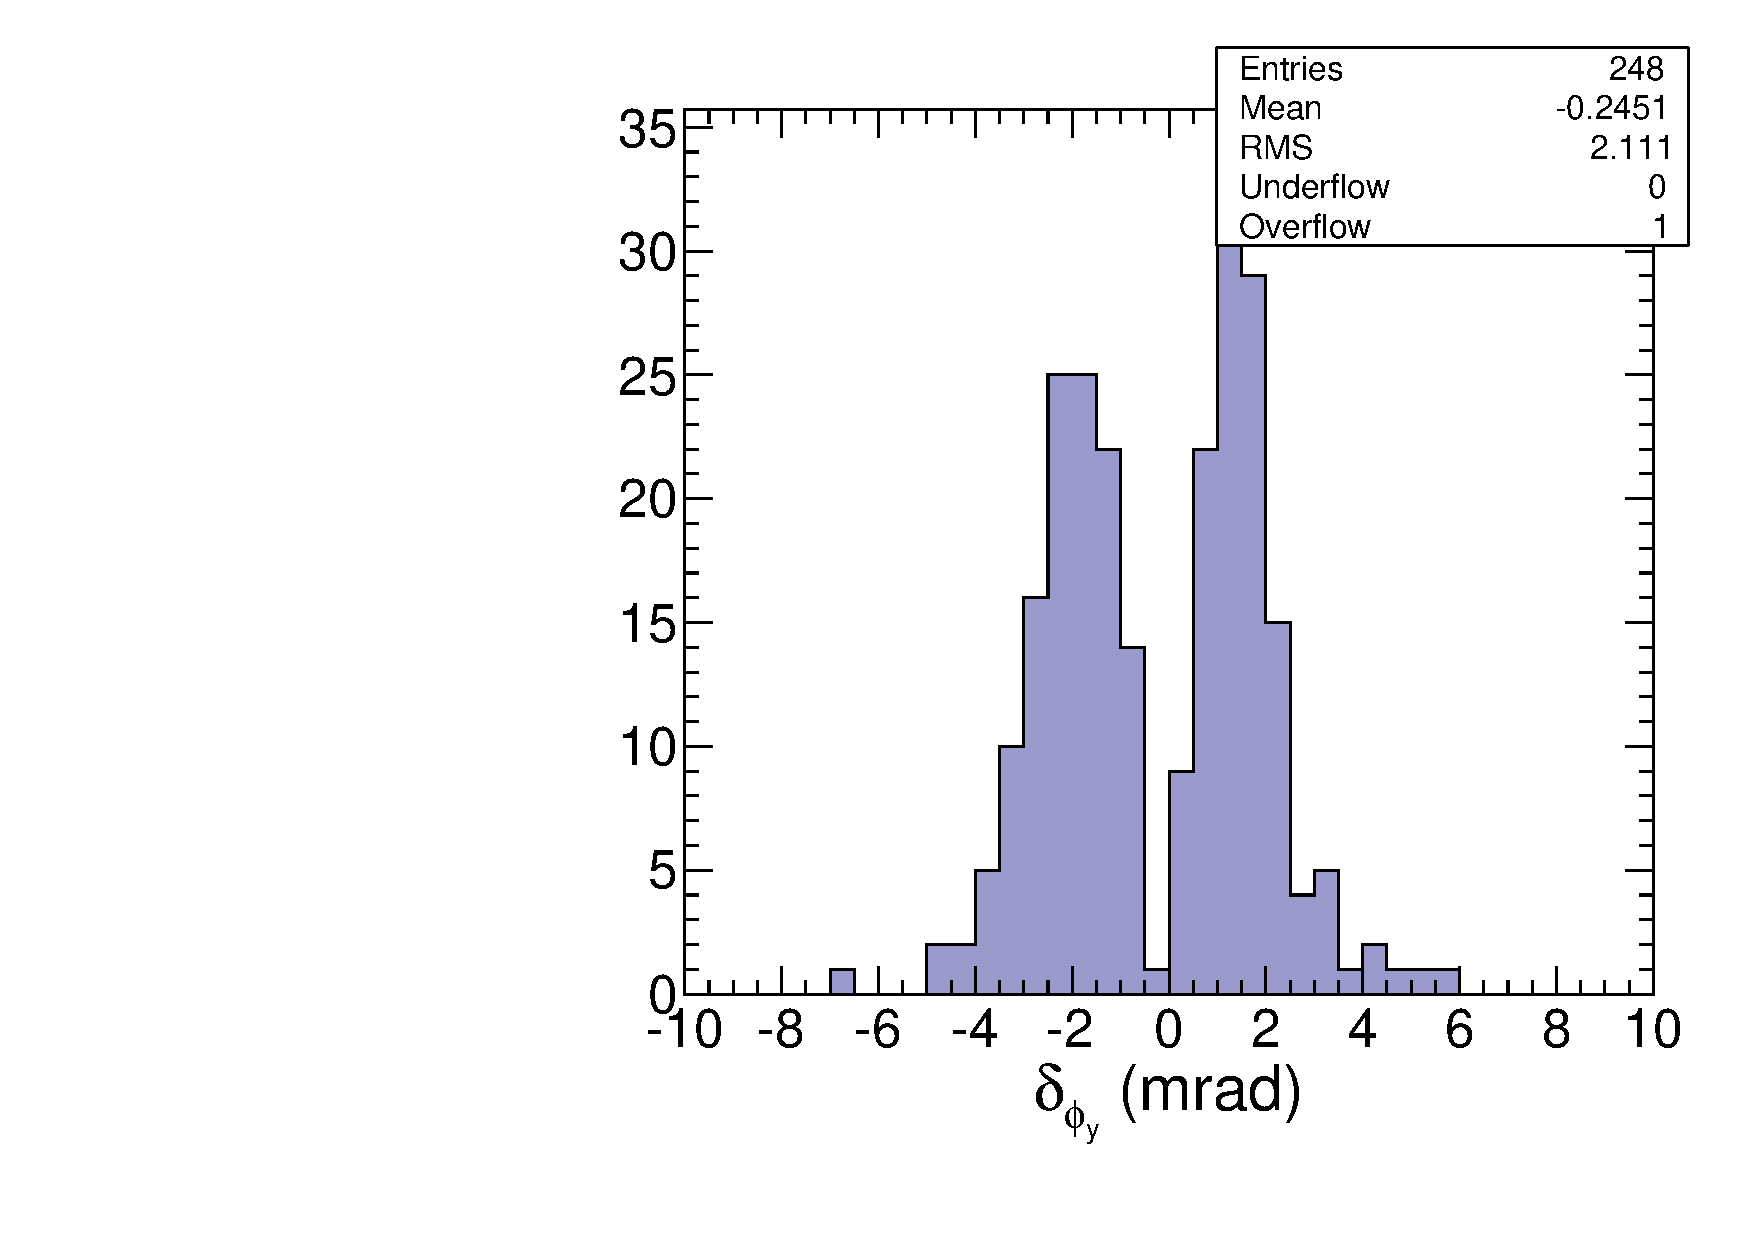
\includegraphics[width=0.5\linewidth]{10_deltaphiy_without_RPC_and_hardware.pdf}
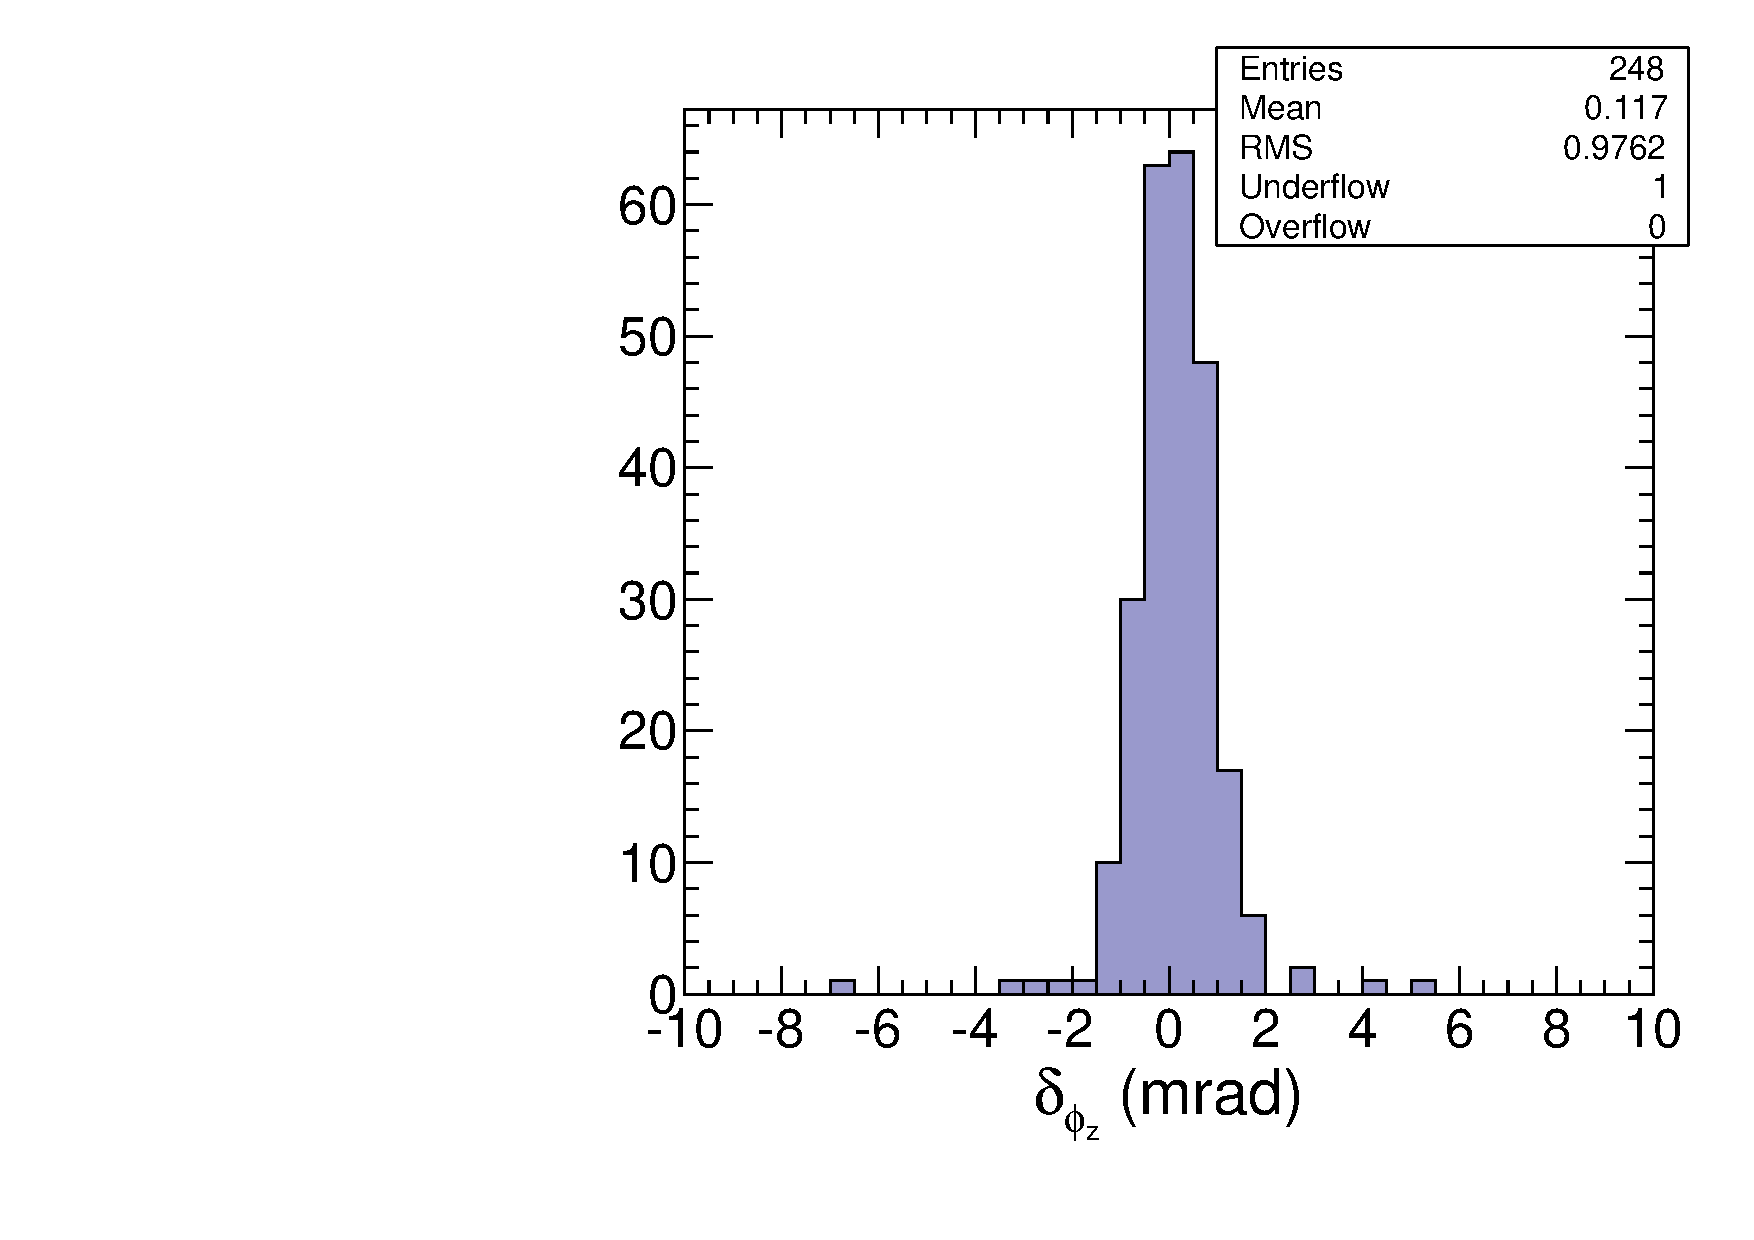
\includegraphics[width=0.5\linewidth]{11_deltaphiz_without_RPC_and_hardware.pdf}

\column{0.3\linewidth}
\begin{itemize}
\item Mostly what we saw last time, except for unaccounted-for global
  rotation
\end{itemize}

\vspace{2 cm}
\hfill \textcolor{darkblue}{\scriptsize CRAFT-10}
\end{columns}
\end{frame}

\begin{frame}
\frametitle{New 2010 muon alignment}

(Comparing alignment without RPC bias to hardware)

\begin{itemize}
\item ``Barrel twist'' is still present with the same magnitude

plus unaccounted-for global rotation
\end{itemize}

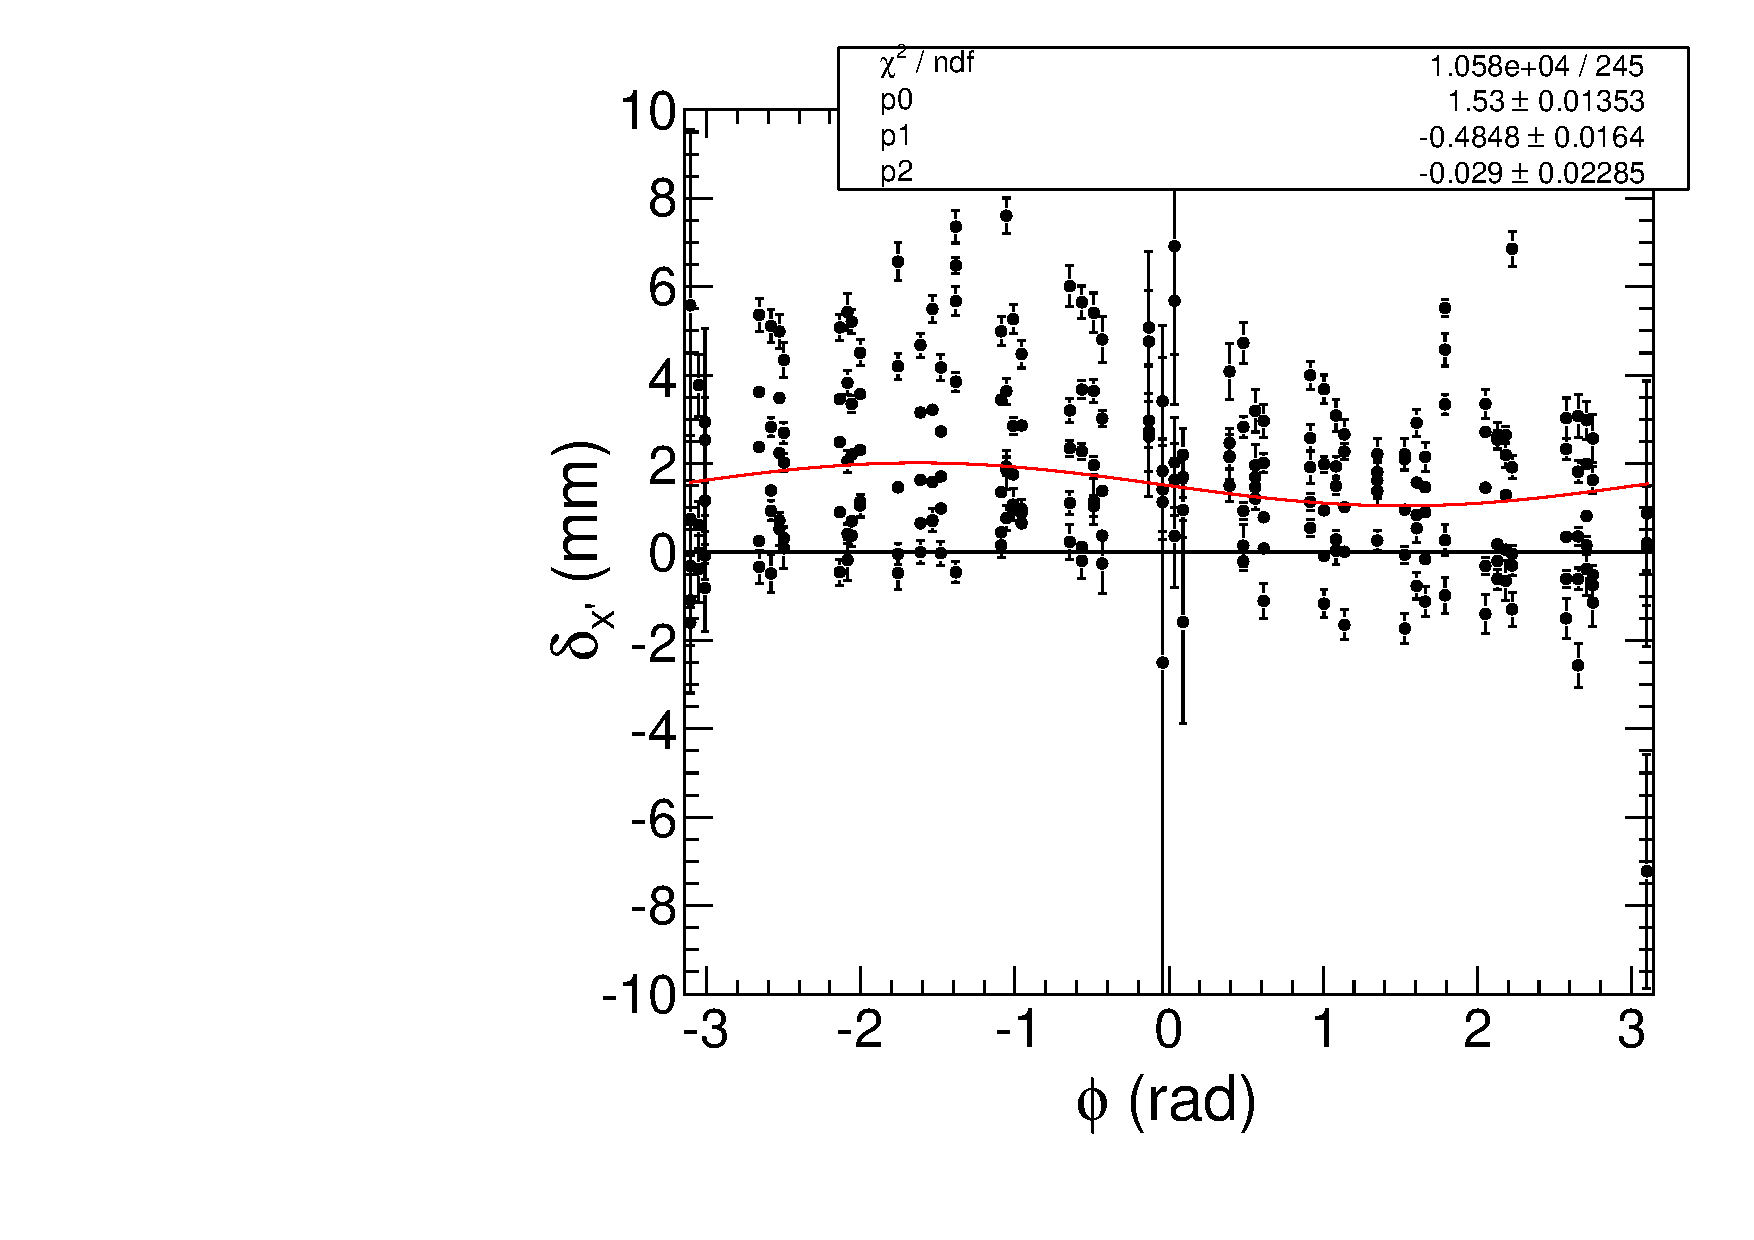
\includegraphics[width=0.5\linewidth]{12_deltax_phi_without_RPC_and_hardware.pdf}
\includegraphics[width=0.5\linewidth]{13_deltax_stack_without_RPC_and_hardware.pdf}

\hfill \textcolor{darkblue}{\scriptsize CRAFT-10}
\end{frame}

\begin{frame}
\frametitle{``Barrel twist'' in residuals}

Unbiased by RPC hits

\vfill
Top of CMS

\vspace{0.2 cm}
\includegraphics[width=0.33\linewidth]{map_1_4.png}
\includegraphics[width=0.33\linewidth]{map_2_4.png}
\includegraphics[width=0.33\linewidth]{map_3_4.png}

\vfill
Bottom of CMS

\vspace{0.2 cm}
\includegraphics[width=0.33\linewidth]{map_1_10.png}
\includegraphics[width=0.33\linewidth]{map_2_10.png}
\includegraphics[width=0.33\linewidth]{map_3_10.png}

\hfill \textcolor{darkblue}{\scriptsize CRAFT-10}
\end{frame}


%% \section*{First section}
%% \begin{frame}
%% \begin{center}
%% \Huge \textcolor{blue}{First section}
%% \end{center}
%% \end{frame}

\begin{frame}
\frametitle{Conclusions}
\begin{itemize}
\item Confirmation: sawtooth and dependence on $q/p_T$ disappear when tracks unbiased by RPC hits
\begin{itemize}
\item $p_T > 100$~GeV/$c$ cut limits effect on alignment results
\end{itemize}

\item We do not see large $\vec{B}$ field bias: less than 1\% before station~1

\item Modified interpretation of tracker weak modes
\begin{itemize}
\item no more ``high-momentum vs.\ low-momentum'' discrepancy
\item muon residuals cannot probe tracker weak modes
\item cosmic endpoint constraint on tracker weak modes $\Rightarrow$
  $\sim$0.25~mm bias in chamber $x$ positions
\end{itemize}

\item New 2010 muon alignment without RPC bias
\begin{itemize}
\item RPC bias effectively a 0.3~mrad rotation and 1.5~mm chamber position error
\item unrelated to ``twist'' with respect to hardware geometry
\end{itemize}

\item We no longer need the $p_T > 100$~GeV/$c$ cut, which will make alignments with collisions possible
\begin{itemize}
\item resolution vs.\ integrated luminosity estimates must be revised
\end{itemize}
\end{itemize}

\label{numpages}
\end{frame}

\end{document}
